\clearpage

% \section{Different performance metrics}\label{apx:metrics-review}

% \todo{Keep? Review and copy-edit necessary.}

% There are many different ways of evaluating the pipeline performance found in the field of pose estimation. Some of the evaluations include the following:
% \begin{itemize}
% \item Intersection over Union (IoU) of the object 3D cloud with a custom threshold classifying it as a good estimate or not (\eg, in the paper~\cite{10.1007/s11263-014-0733-5} the threshold score above 0.5 is considered good estimation).
% \item Translation and rotation error between estimated 3D model and true 3D model with fixed thresholds (\eg, in the paper~\cite{shotton2013scene} they require the translation error to be below 5 cm and rotation error to be below 5\degree)
% \item The average distance of all the points of the model from their transformed version, and if the error is less than the constant multiple of diameter of the 3D model, it is considered correctly evaluated (\eg, evaluation error is used in papers~\cite{10.1007/978-3-642-37331-2_42, xiang2018posecnn})
% \item Reprojection error that projects the estimated points onto the image and computes the pairwise distances in the image space, instead of computing distances in the 3D model space (\eg, used in paper~\cite{xiang2018posecnn})
% \item The recovery error measured as Frobenius norm from estimated 3D model and true model, where 3D model is composed of 3D locations of important landmarks (\eg, elbow for human pose estimation)~\cite{wangni2018monocular}
% \item Average Orientation Similarity (AOS) is the difference between the true and estimated model with a cosine similarity term~\cite{RedondoCabrera2016PoseEE}
% \item Mean Angle Error (MAE) and Median Angle Error (MedError) evaluated and compared with other pose estimation error metrics in the paper~\cite{RedondoCabrera2016PoseEE}.
% \end{itemize}

\section{Sampling of orientations}\label{apx:orientation-sampling}

%\todo{What do we want to say here? Sampling of orientations, or sampling of distances?}

\figref{orientation-sampling} shows four distributions of orientations and the distributions of distances they induce.
%While the distributions distances for partial coverages of directions flatten (compared with both full direction coverage), the shorter distances are still under-sampled.
As shorter distances are under-sampled, we uniformly resampled the distances to avoid biasing the training of our distance estimator.

While we control the distributions of orientations and distances to facilitate distance learning, we cannot control them when recovering orientations of a given set of projections.
Comparing Figure~\ref{fig:nonuniform:recovery} with~\ref{fig:5j0n-noise0-orientation-recovery}, and~\ref{fig:nonuniform:reconstruction} with~\ref{fig:5j0n-reconstruction-fsc}, shows that the recovered orientations and the reconstructed density are barely affected by a non-uniform sampling of orientations---a condition that might happen in real cryo-EM acquisitions.

%\banjac{I remember putting somewhere that we have support for both, but I don't see it. I can put a histogram and respective $S^2$ space visualization in the appendix that will visualize the difference. Why we used it? From the log I see that OR was not converging to 0 so we thought is is because we have underestimated learned distance. Shortly after, the OR started working and we didn't continue further with this idea.}

\begin{figure}[ht!]
    \centering
    \begin{minipage}{.33\linewidth}
        \begin{subfigure}[b]{\linewidth}
            \centering
            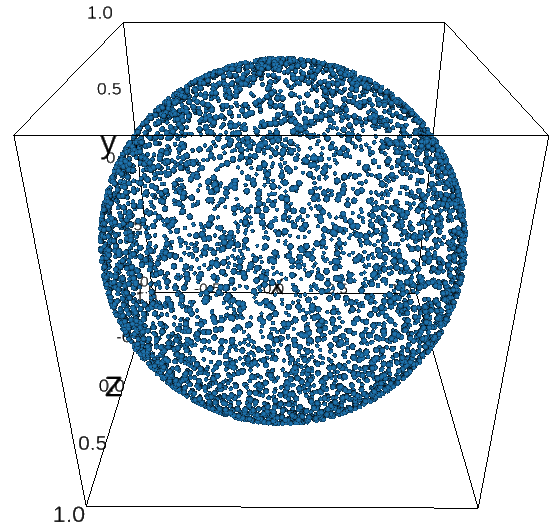
\includegraphics[height=2.5cm]{figures/uniform_quaternion.png}%
            \hfill
            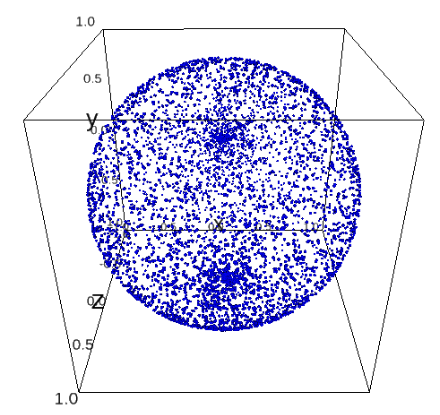
\includegraphics[height=2.5cm]{figures/uniform_angles.png}
            \\ \vspace{0.2cm}
            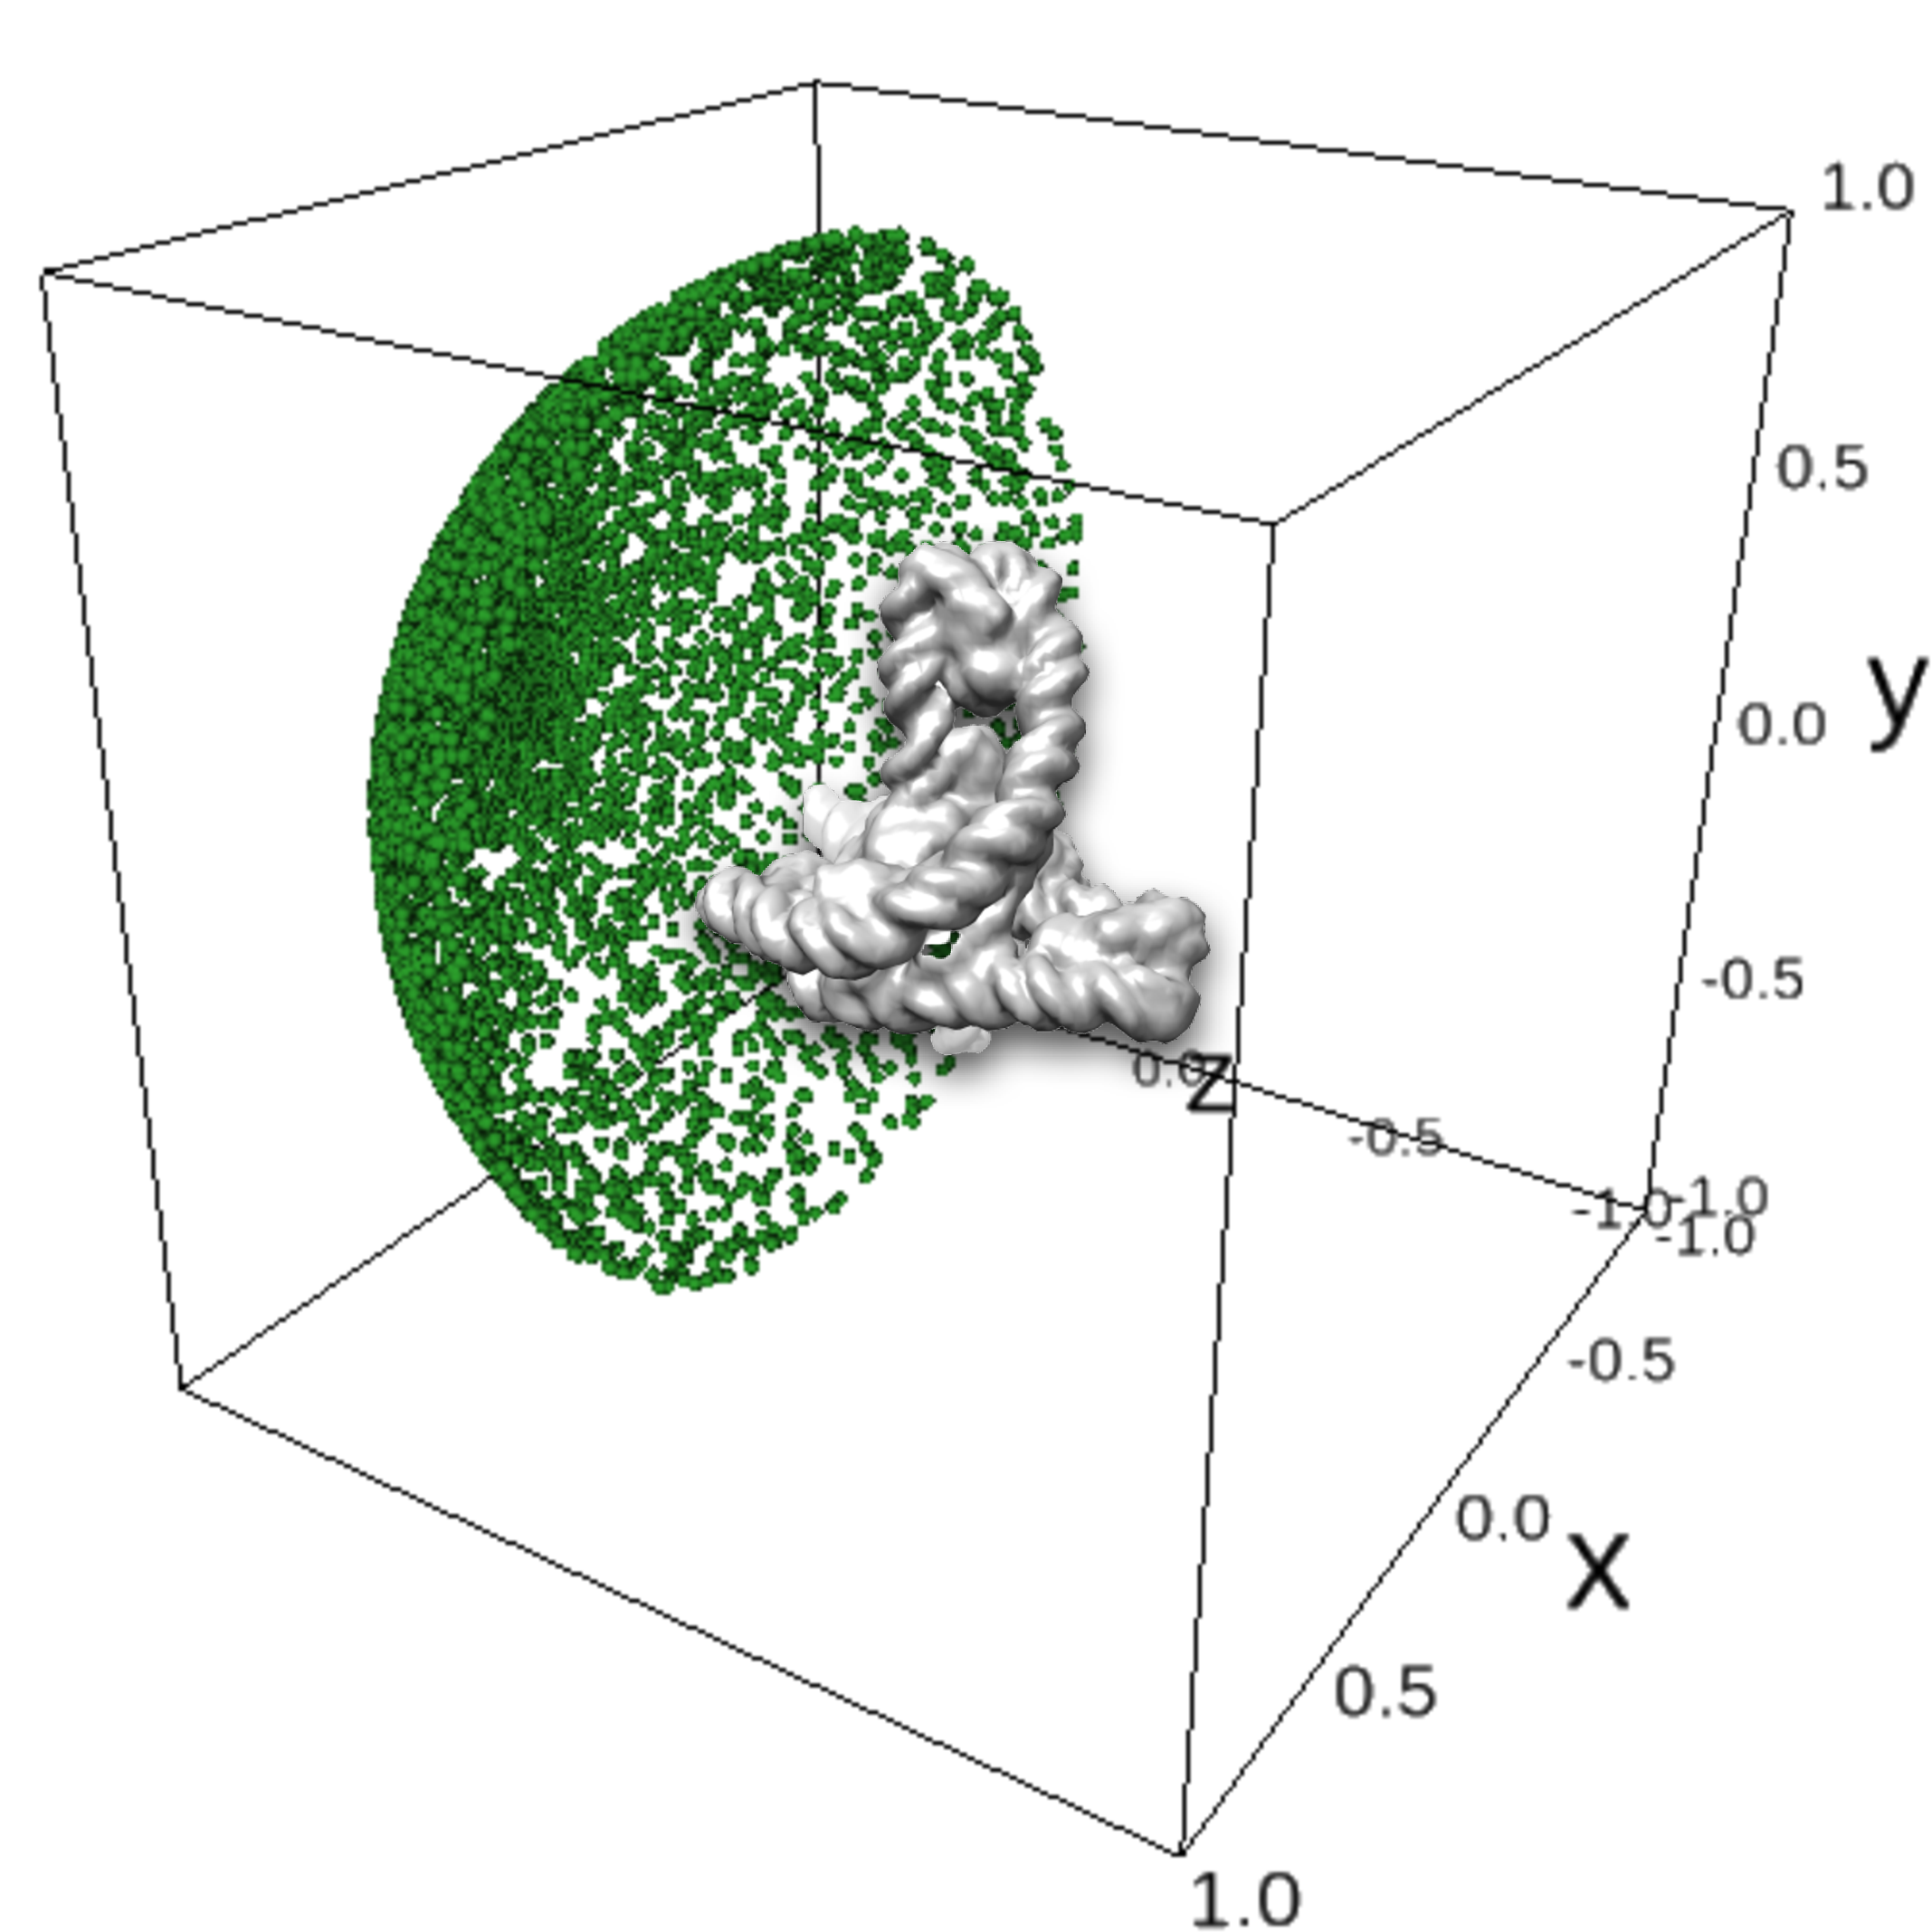
\includegraphics[height=2.5cm]{figures/5j0n-cvg2.pdf}
            \hfill
            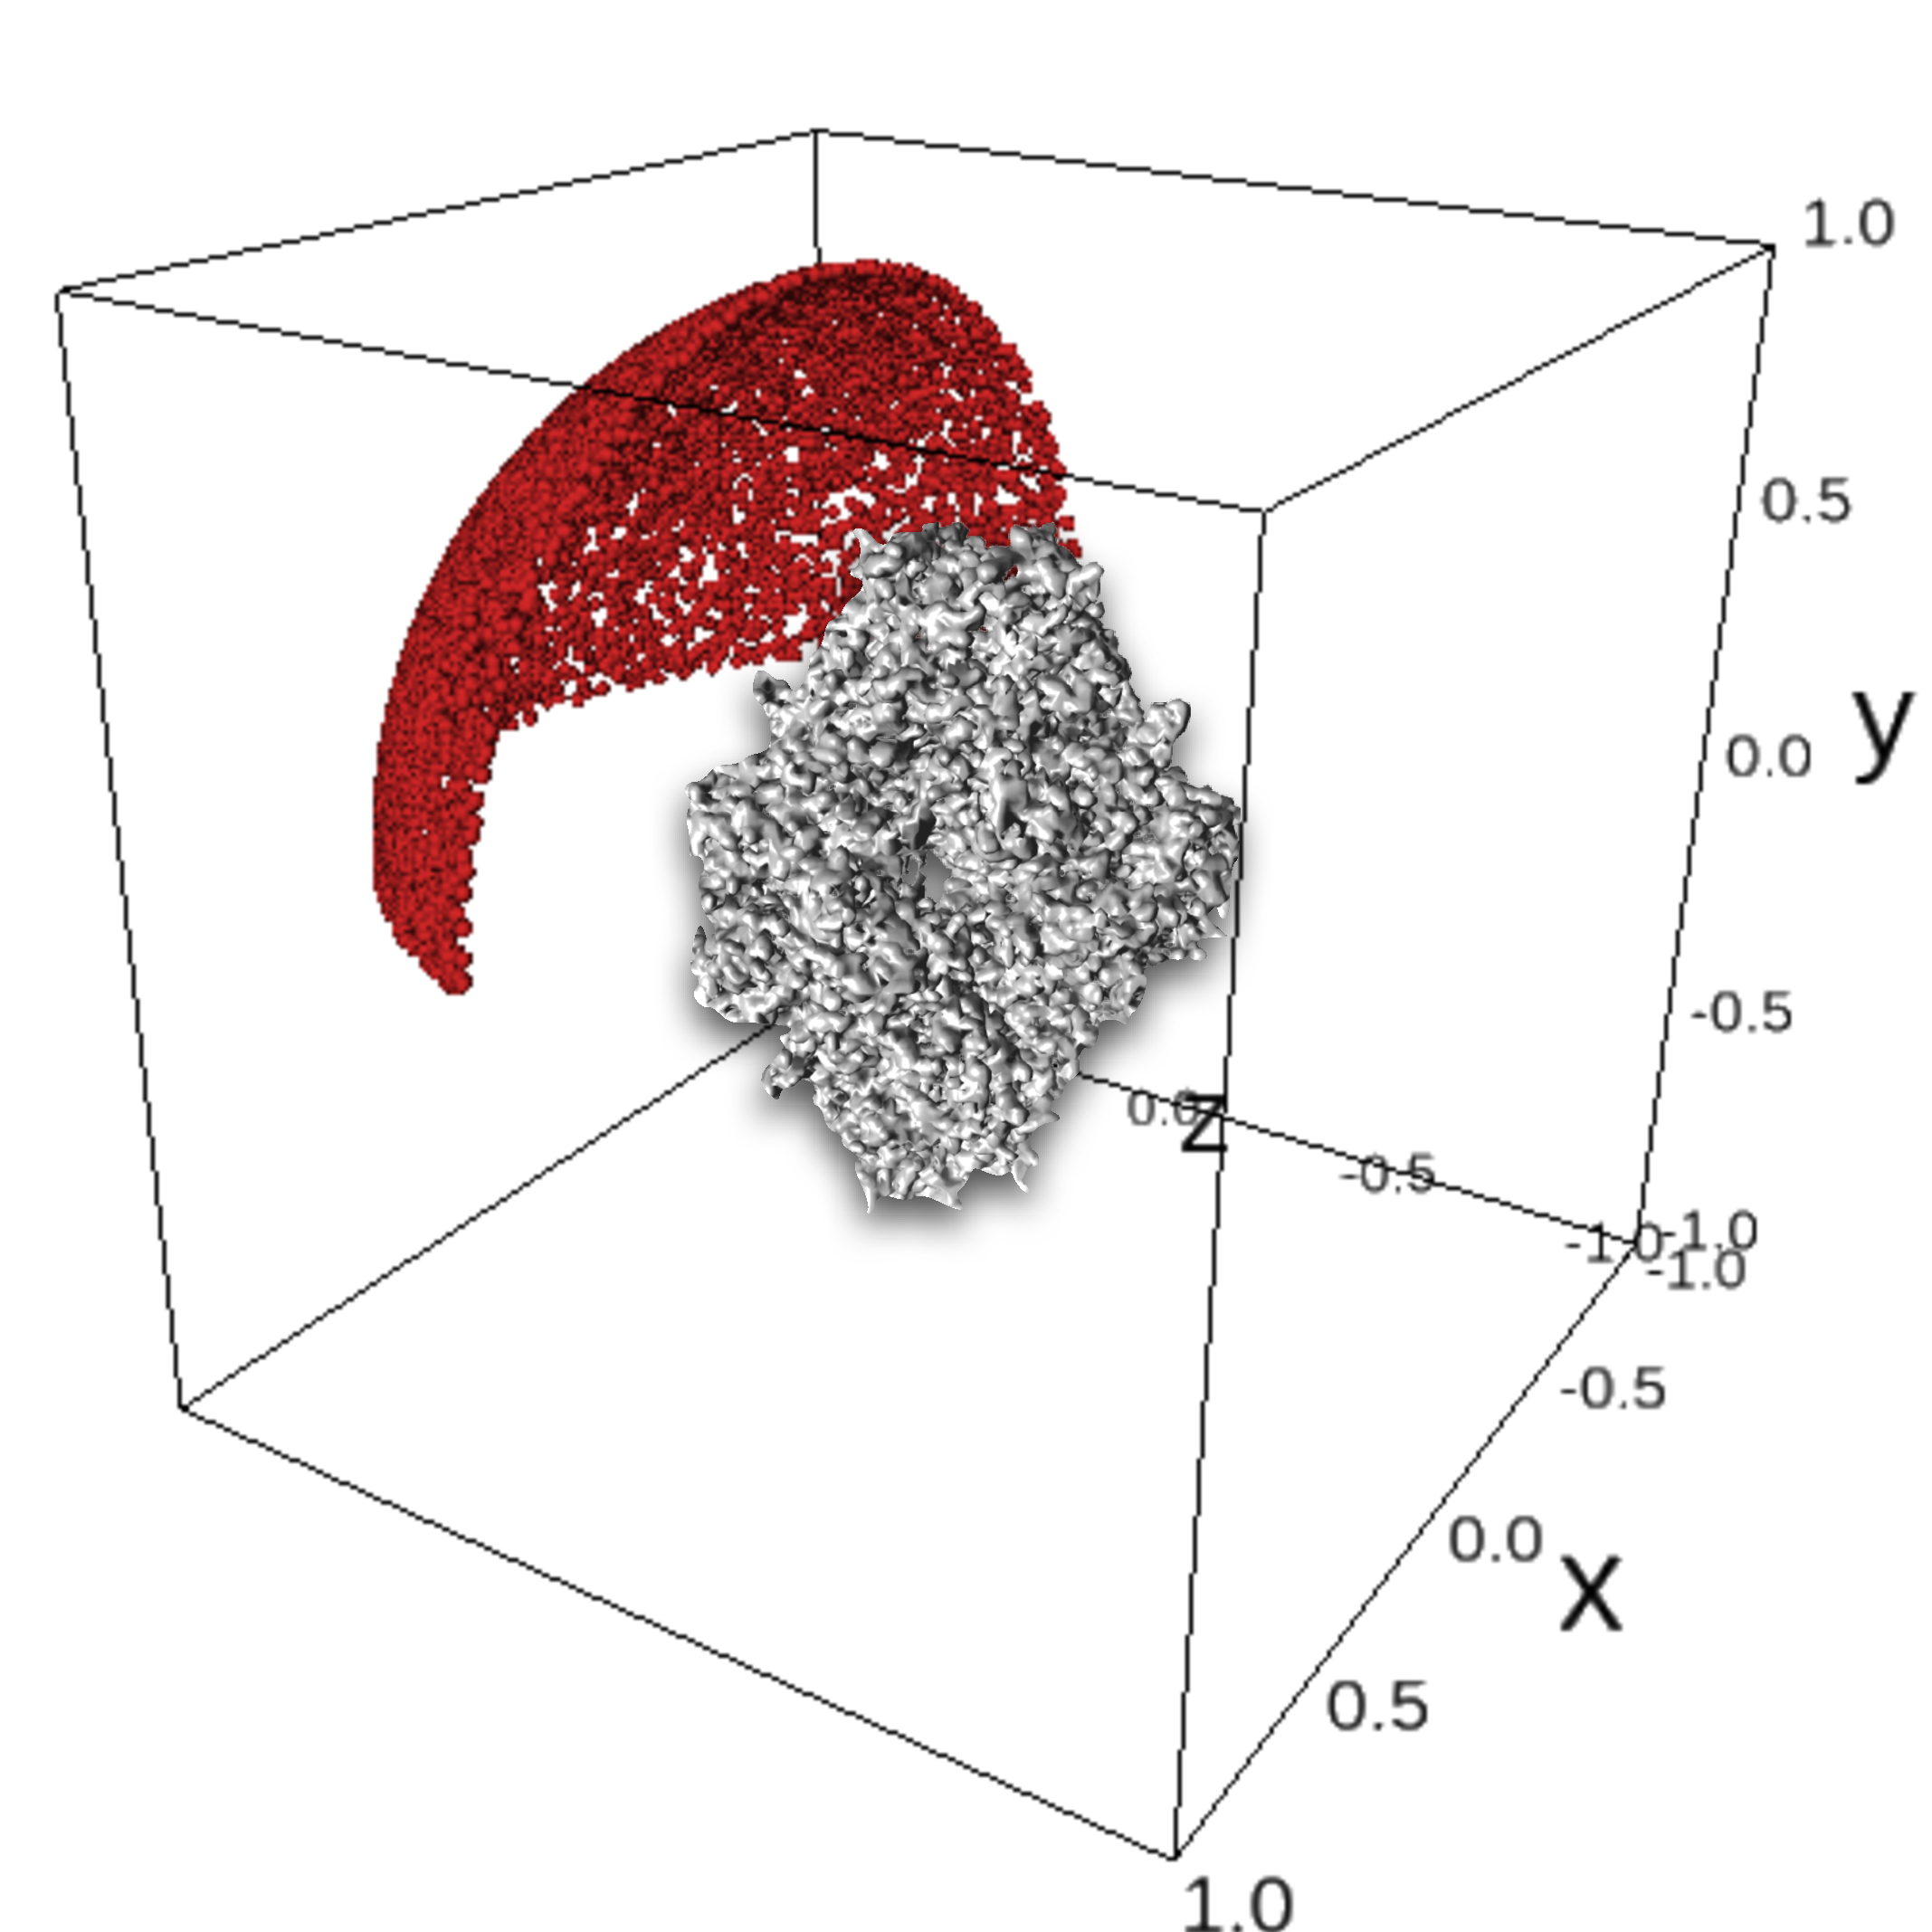
\includegraphics[height=2.5cm]{figures/5a1a-cvg2.pdf}
            \caption{Sampled directions $(\theta_2, \theta_1)$.}%
            \label{fig:orientation-sampling:directions}
        \end{subfigure}
    \end{minipage}
    \hfill
    \begin{minipage}{.65\linewidth}
        \begin{subfigure}[b]{0.37\linewidth}
            \centering
            % 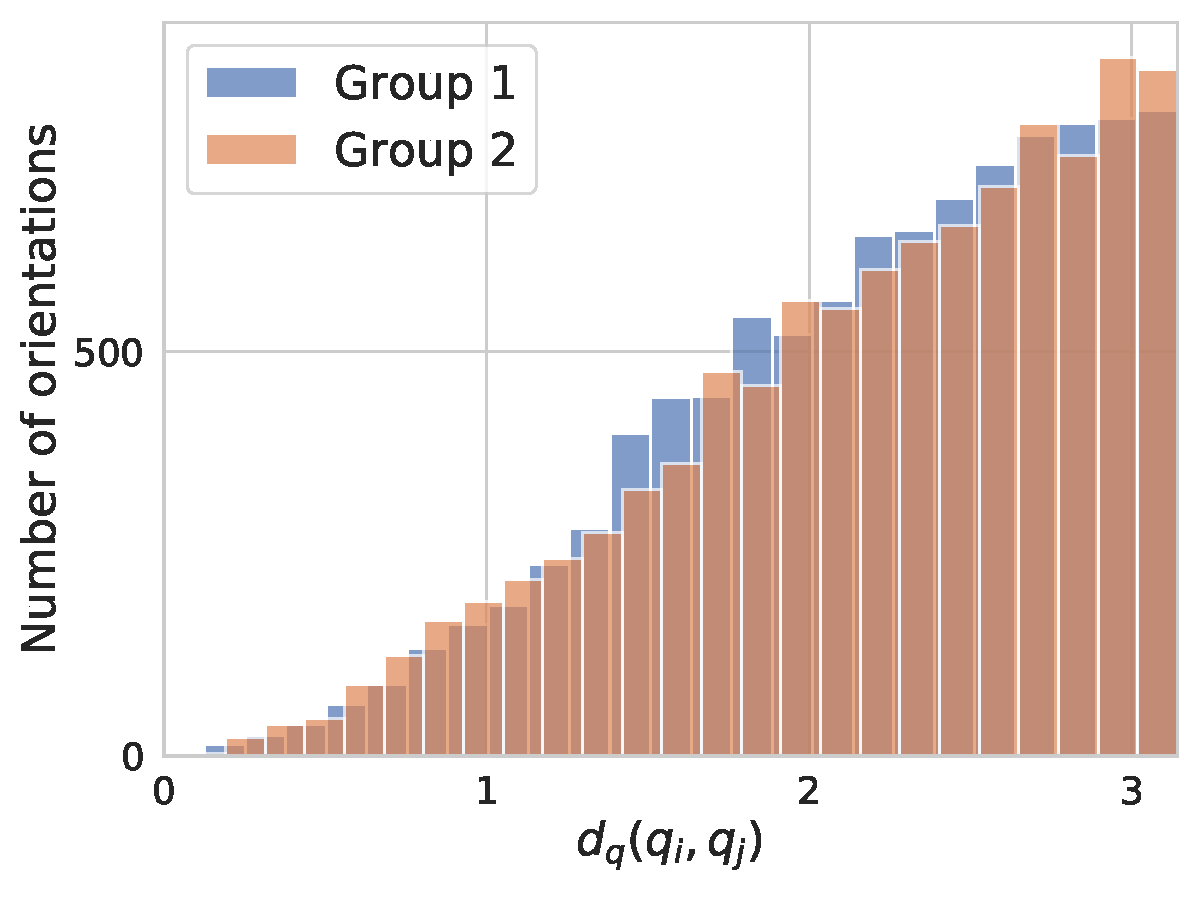
\includegraphics[height=8em]{figures/dQ_5j0n_uniform_quaternions_vs_angles.pdf}
            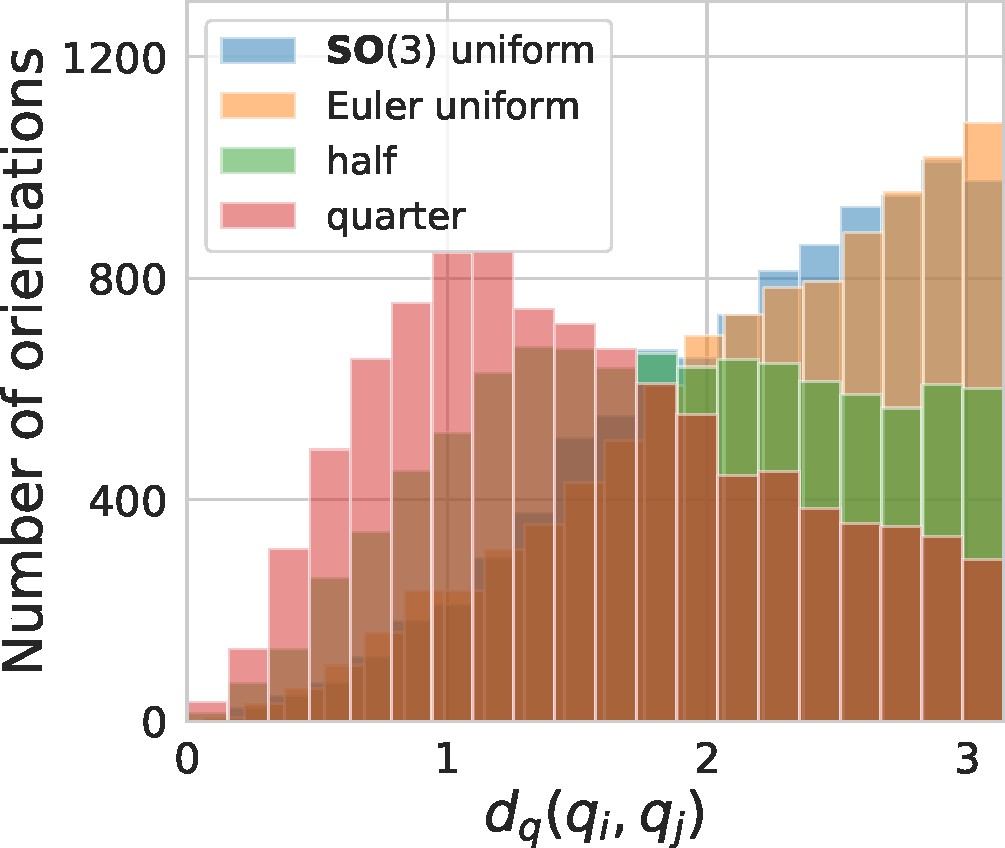
\includegraphics[height=2.4cm]{figures/dQ_distribution_coverage.pdf}
            \caption{Distribution of distances $d_q$.}%
            \label{fig:orientation-sampling:distances}
            \vspace{0.2cm}
        \end{subfigure}
        \hfill
        \begin{subfigure}[b]{0.6\linewidth}
            \centering
            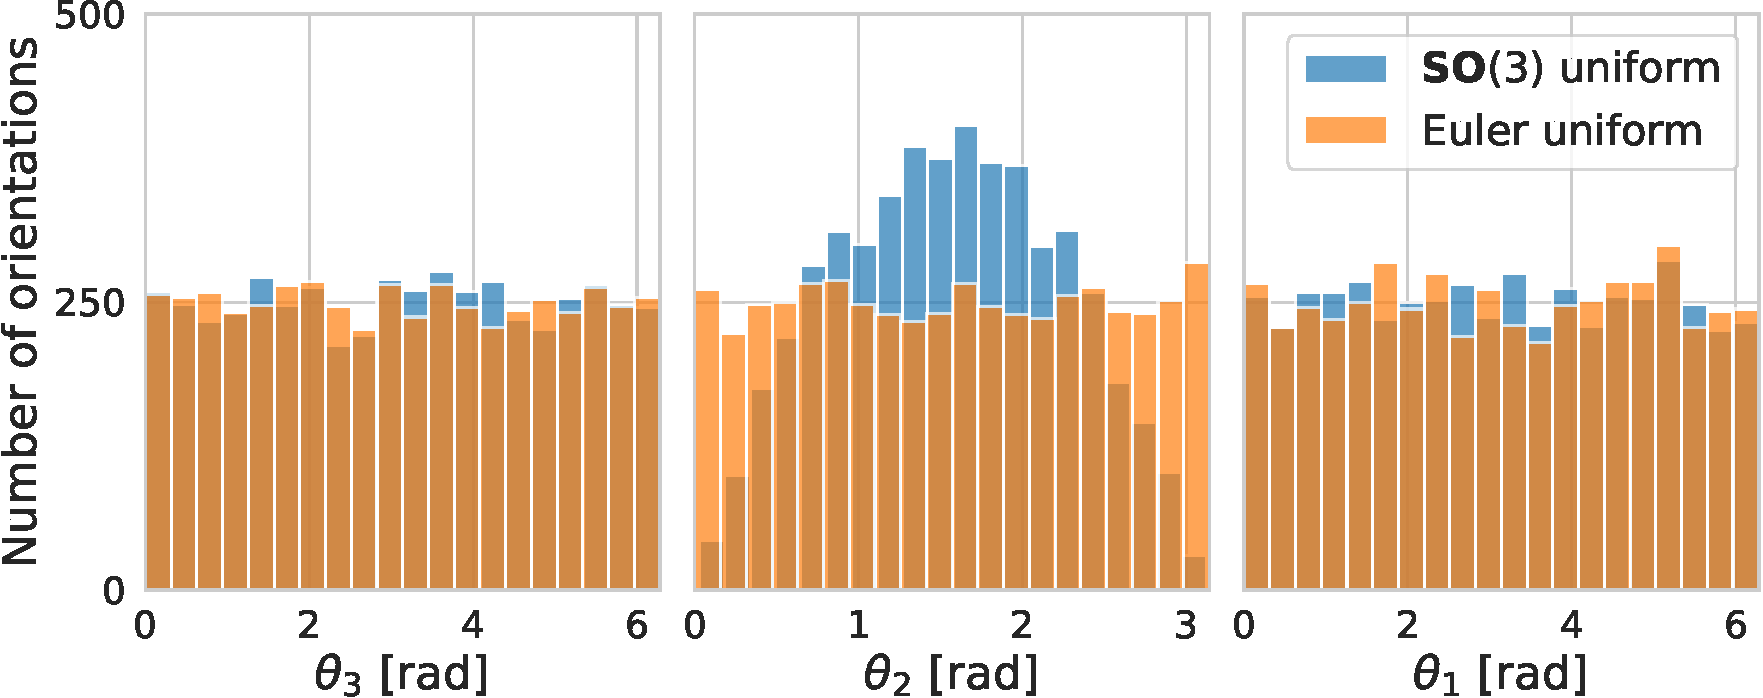
\includegraphics[height=2.4cm]{figures/uniform_quaternions_vs_angles_ang.pdf}
            \caption{Distribution of Euler angles $\bth = (\theta_3,\theta_2,\theta_1)$.}%
            \label{fig:orientation-sampling:angles}
            \vspace{0.2cm}
        \end{subfigure}
        \begin{subfigure}[b]{0.97\linewidth}
            \centering
            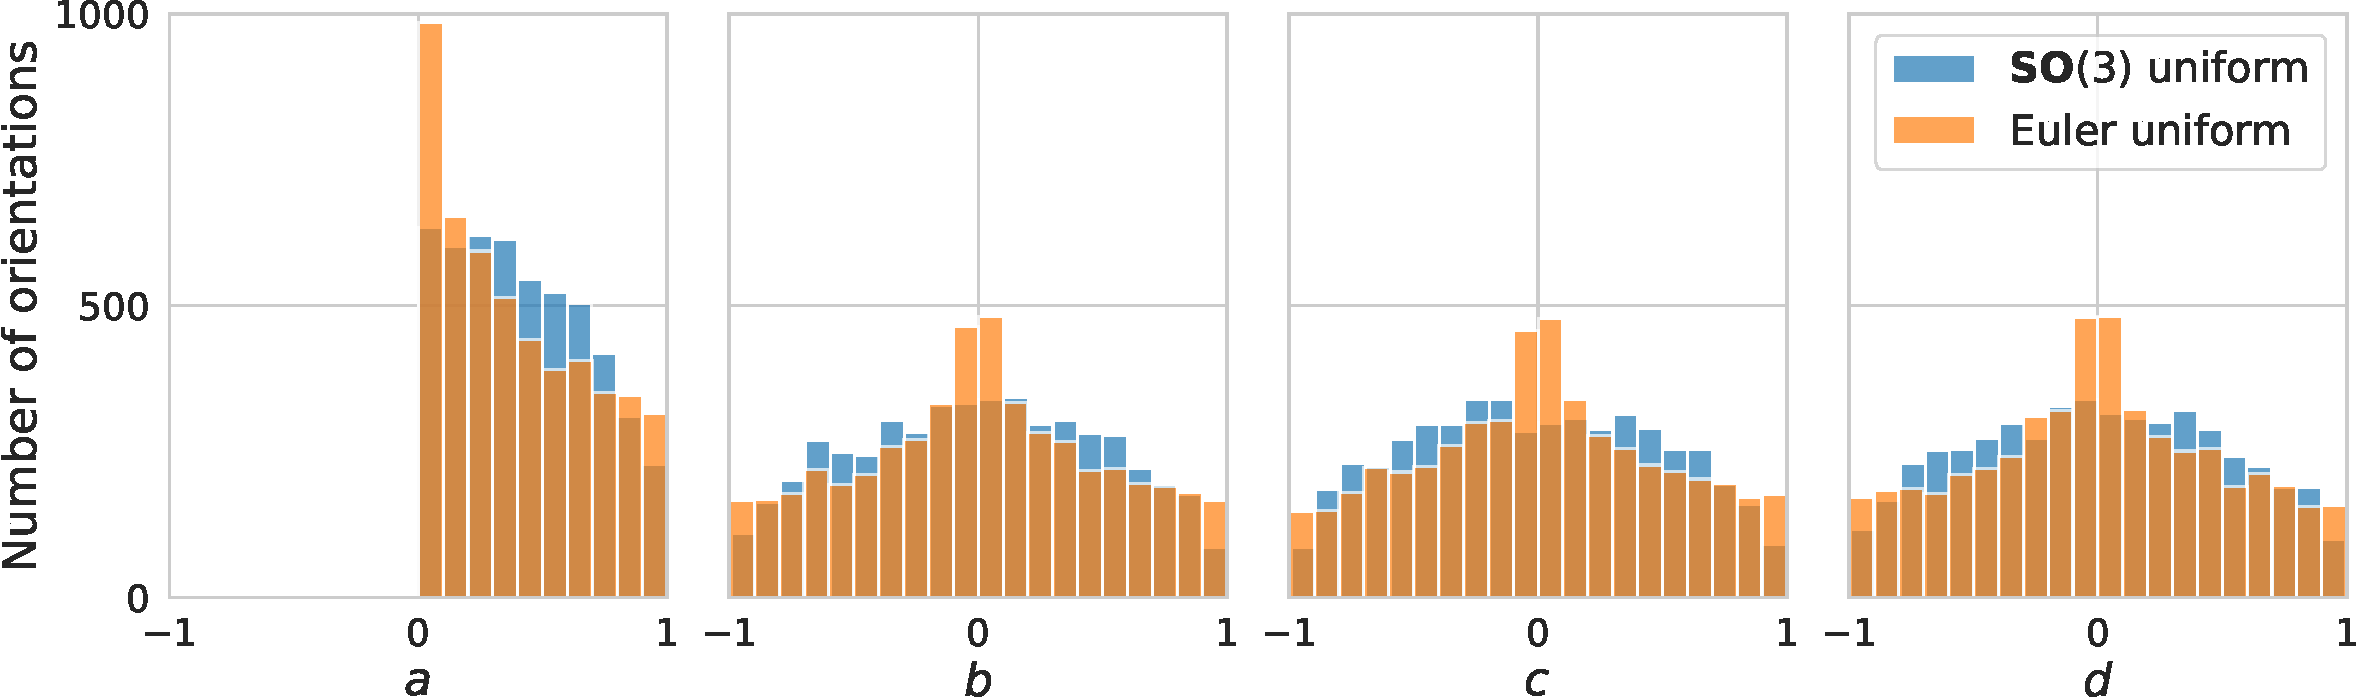
\includegraphics[height=2.4cm]{figures/uniform_quaternions_vs_angles_q.pdf}
            \caption{Distribution of quaternions $q = a + b\boldsymbol{i} + c\boldsymbol{j} + d\boldsymbol{k}$.}%
            \label{fig:orientation-sampling:quaternions}
        \end{subfigure}
    \end{minipage}
    \caption{%
        % ($P < 10,000$)
        Sampling of orientations from four distributions:
        %illustrating their constrained range, and the distances they induce:
        (blue) uniform on $\SO(3)$, (orange) uniform on Euler angles, (green) Euler uniform restricted to half the directions $(\theta_2, \theta_1) \in [0,\frac{\pi}{2}[ \, \times \, [0,2\pi[$, and (red) $\SO(3)$ uniform restricted to a quarter of the directions $(\theta_2, \theta_1) \in [0,\frac{\pi}{2}[ \, \times \, [0,\pi[$.
    }\label{fig:orientation-sampling}
\end{figure}

\begin{figure}[ht!]
    \centering
    \begin{subfigure}[b]{0.48\linewidth}
        \centering
        % 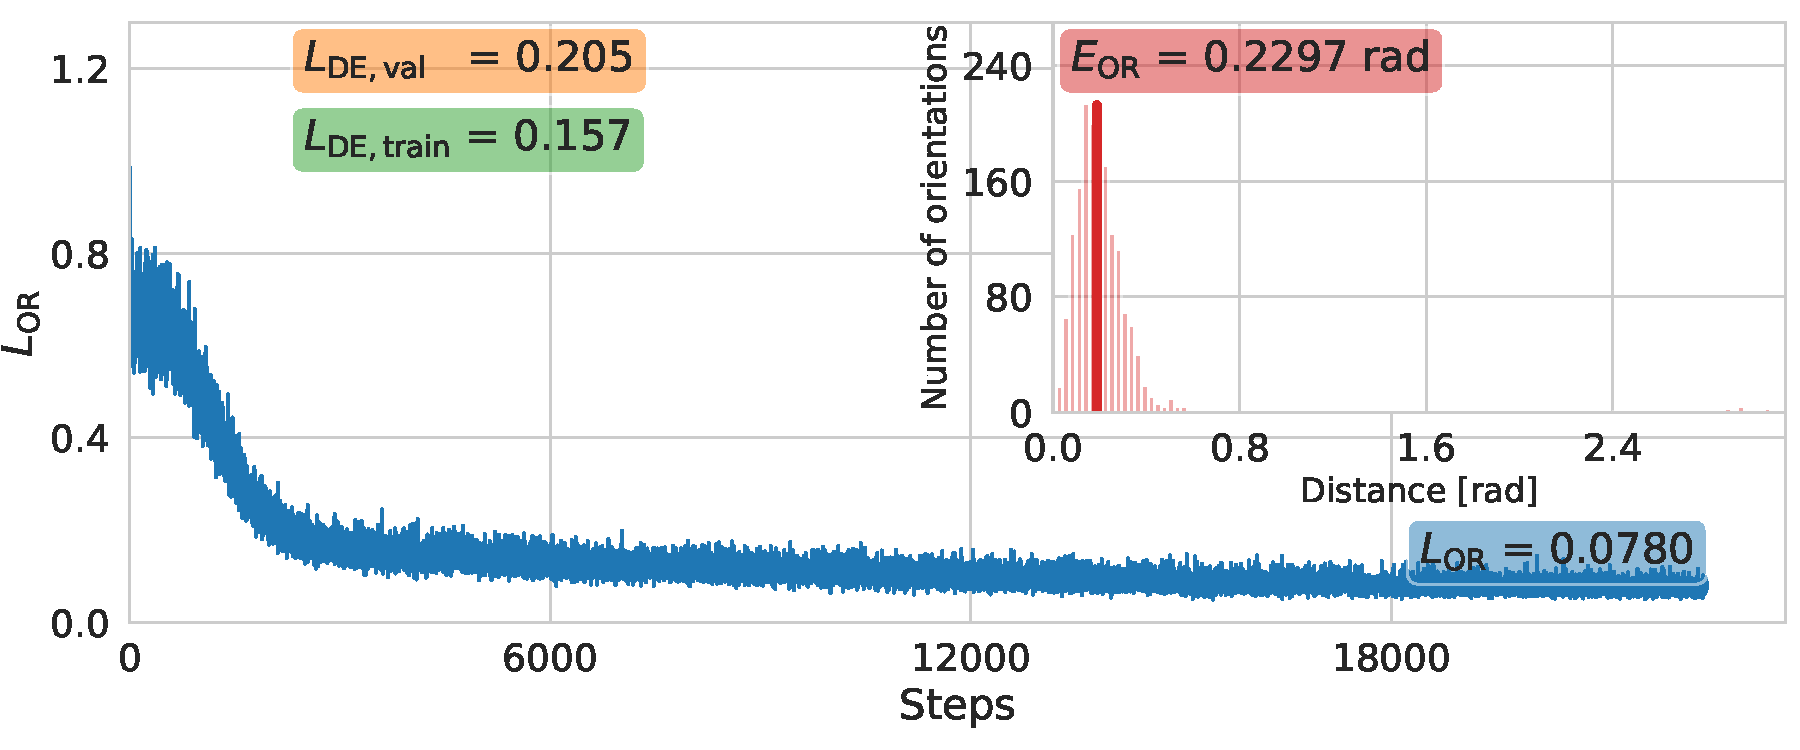
\includegraphics[height=3cm]{figures/5j0n_ar_aa_fullcvg.pdf}
        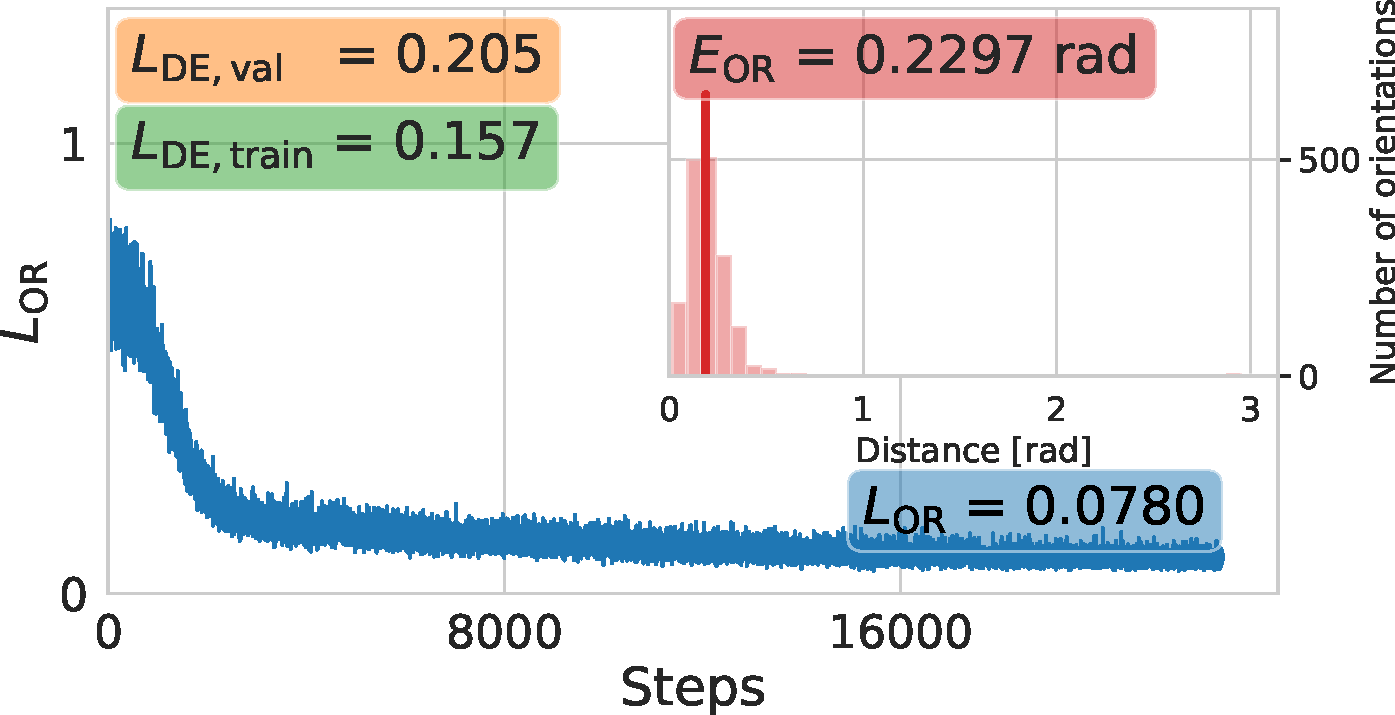
\includegraphics[height=3cm]{figures/5j0n_ar_aa_fullcvg_smaller.pdf}
        \caption{Distance learning and orientation recovery.}%
        \label{fig:nonuniform:recovery}
    \end{subfigure}
    \hfill
    \begin{subfigure}[b]{0.48\linewidth}
        \centering
        % 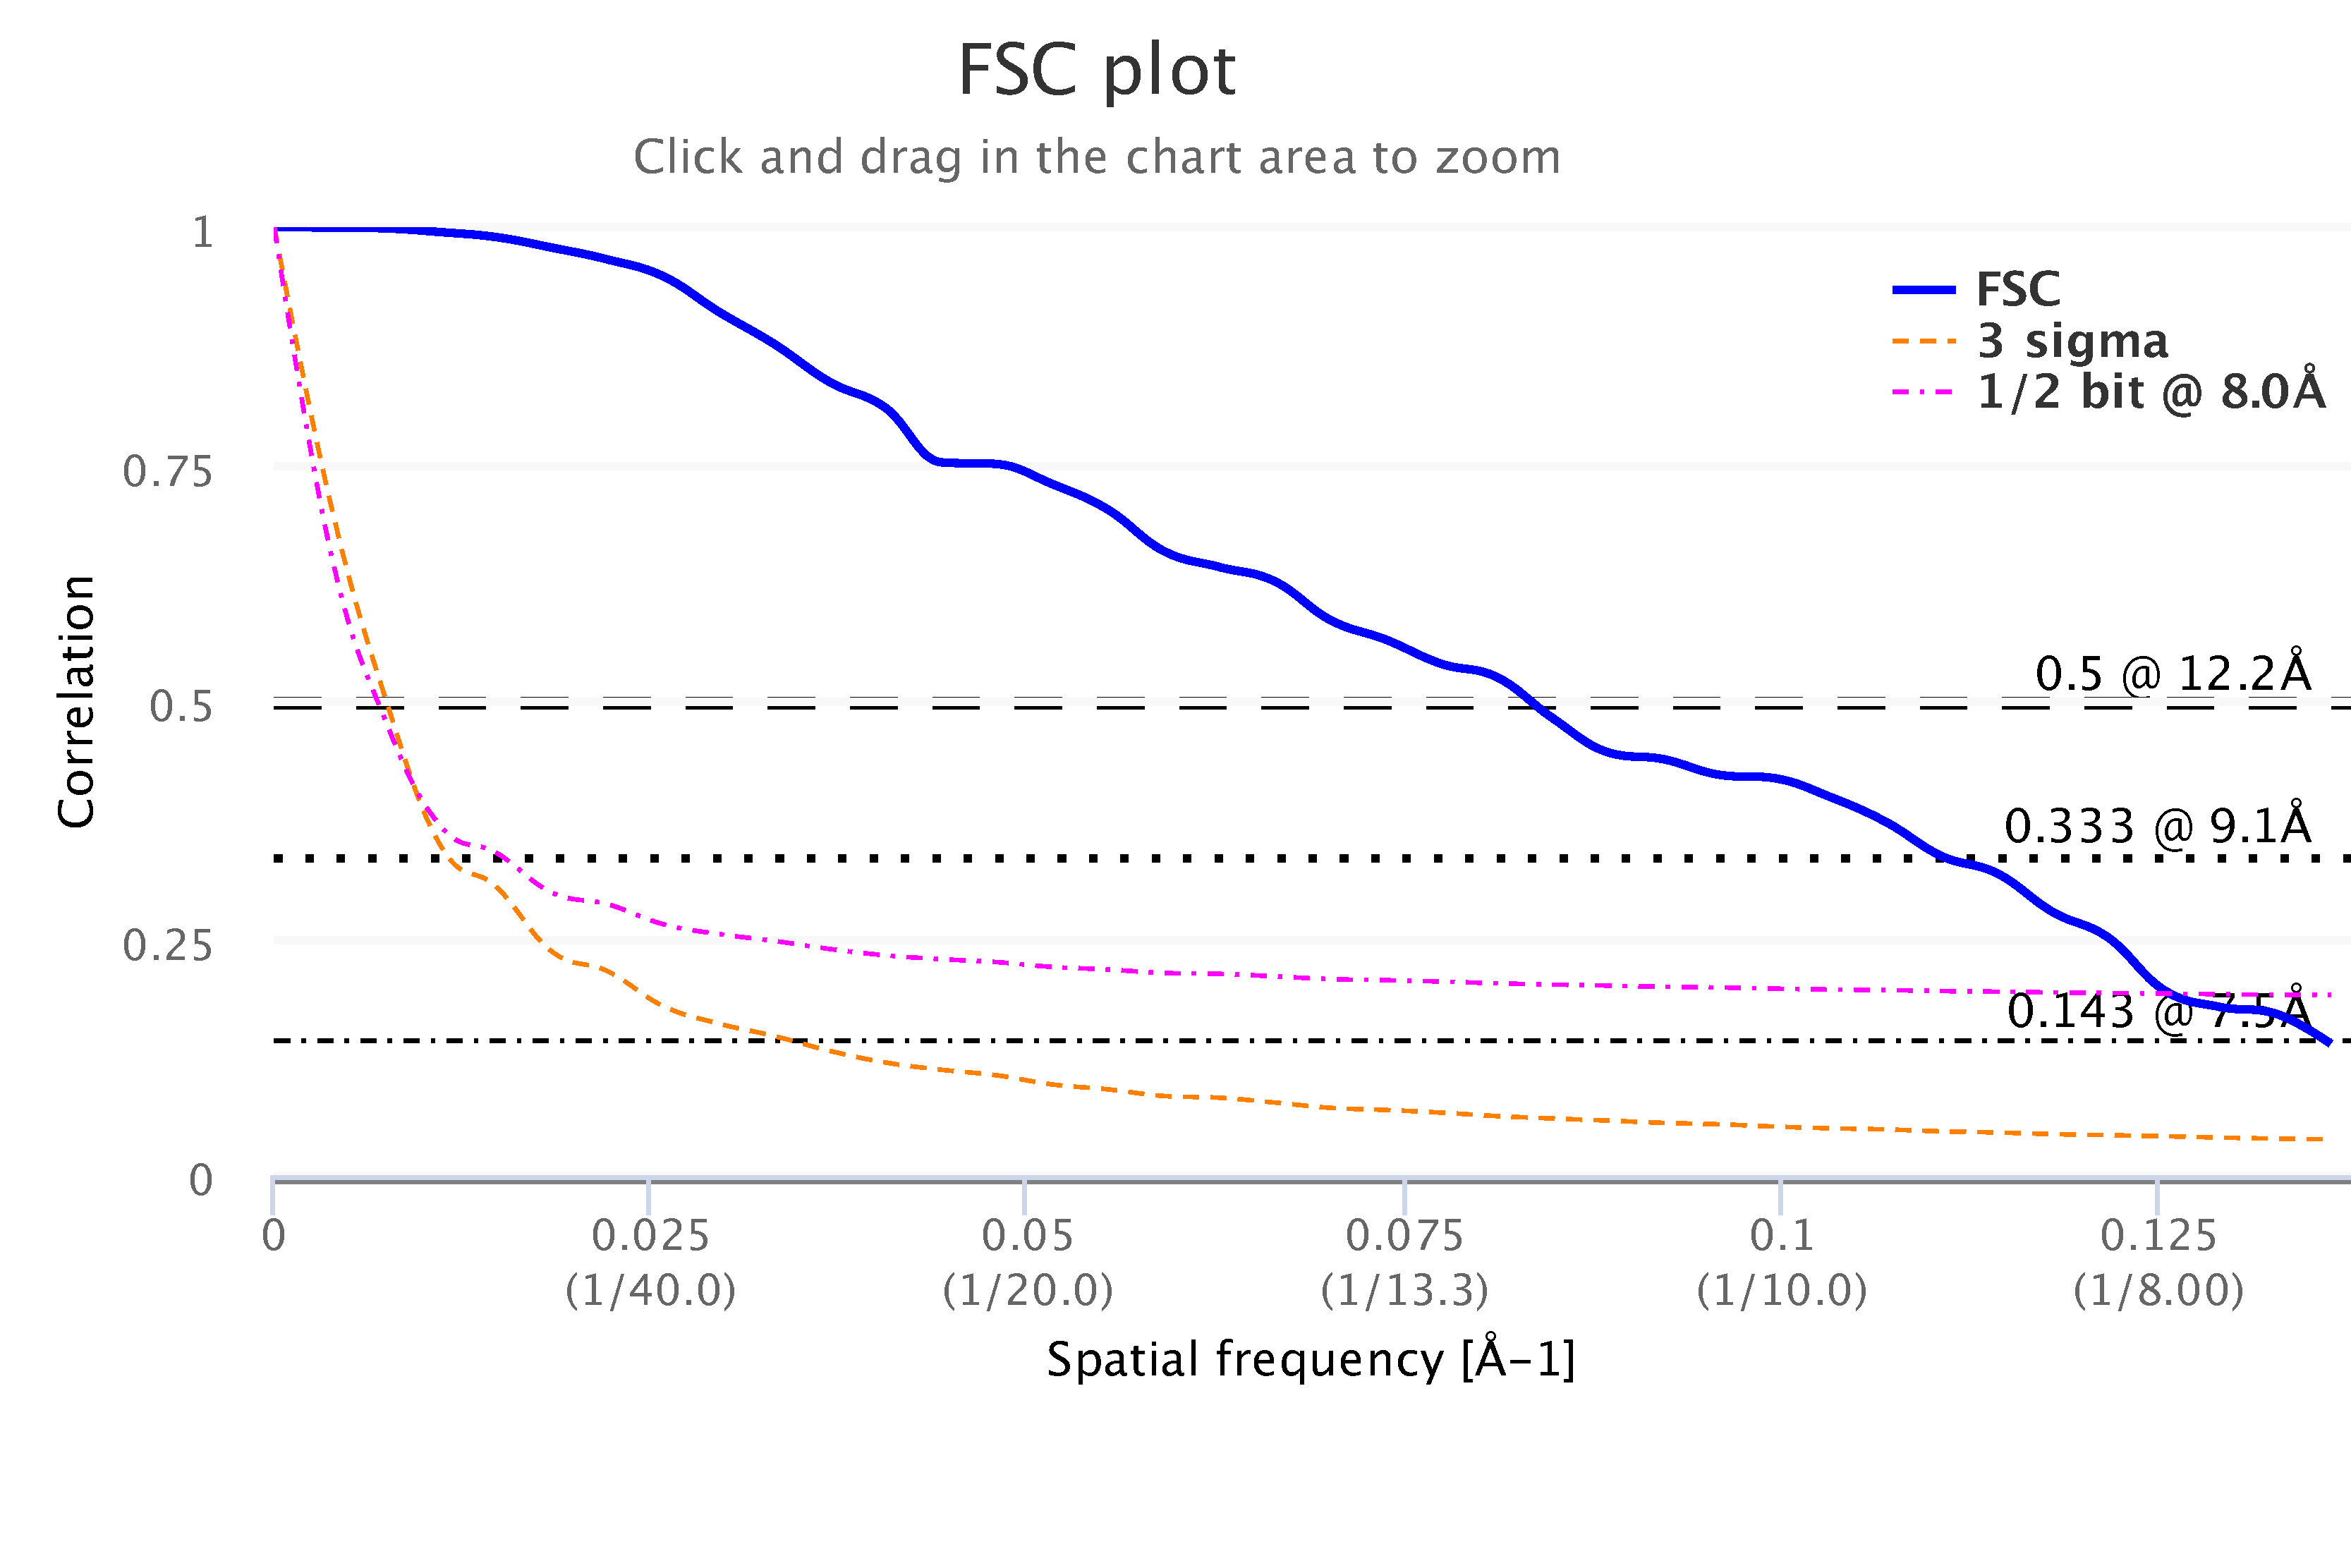
\includegraphics[height=4cm]{figures/FSC_5j0n_fullcvg_noise0_fin_vs_init.pdf}
        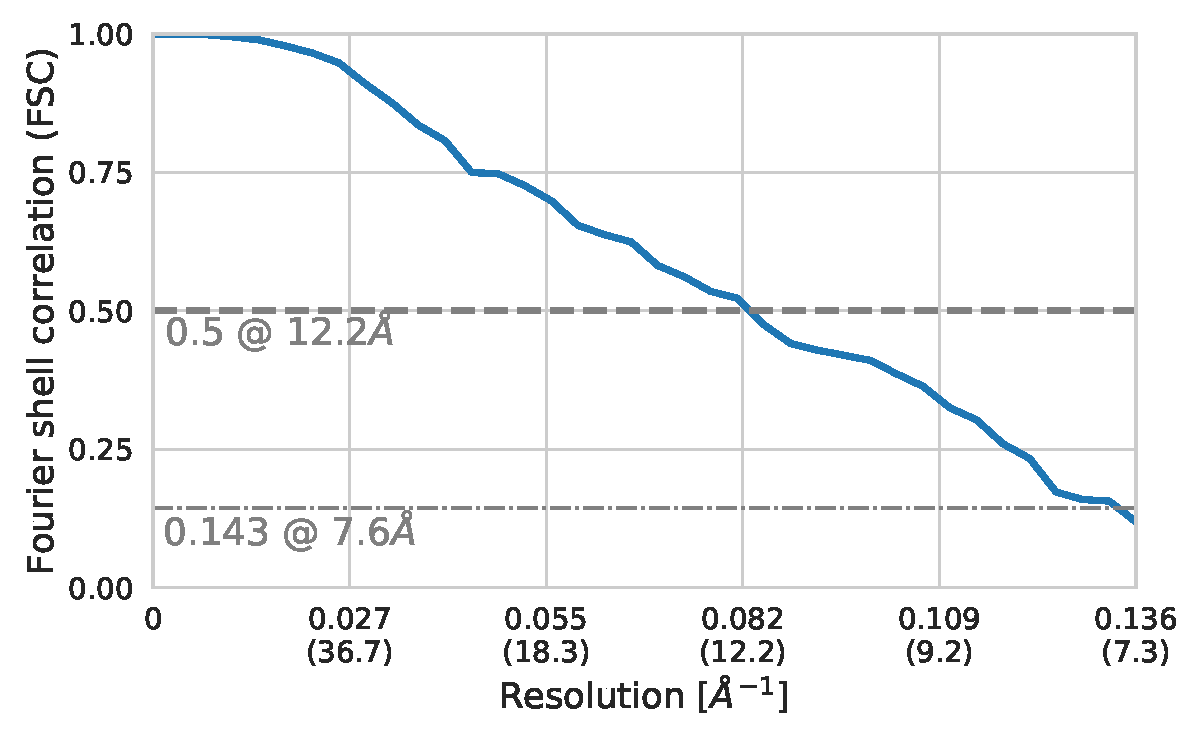
\includegraphics[height=3cm]{figures/5j0n_fullcvg_noise0_FSC_apr_init_customFSC.pdf}
        \caption{Fourier shell correlation (FSC) of the reconstructed density.}%
        \label{fig:nonuniform:reconstruction}
    \end{subfigure}
    \caption{%
        Orientation recovery and density reconstruction from noiseless projections of \texttt{5j0n} acquired from non-uniformly sampled orientations (uniformly sampled Euler angles, \figref{orientation-sampling} (orange)).
        %Full pipeline on the orientations with uniform sampling of Euler angles from full 2-sphere coverage.
    }
\end{figure}

\section{Orientation recovery from exact distances}\label{apx:results:orientation-recovery:exact}

%\mdeff{Story: works perfectly despite no convexity guarantee and sampling.}

To verify that the lack of a convexity guarantee for \eqnref{orientation-recovery} and the sampling of the sum are non-issues in practice, we attempted orientation recovery under exact distance estimation $\widehat{d_p}(\p_i, \p_j) = d_q(q_i, q_j)$.
Orientations were perfectly recovered;
\figref{5j0n-orientation-recovery-loss} shows the convergence of $L_\text{OR}$ to zero.
\figref{5j0n-aa-loss-perfect-distances} shows how~\eqnref{orientation-recovery-error} could then perfectly align the recovered and true orientations---leading to $E_\text{OR} = 0$.
It illustrates how alignment is necessary to evaluate the performance of orientation recovery.

\begin{figure}[ht!]
    \begin{minipage}[t]{0.30\linewidth}
        \centering
        %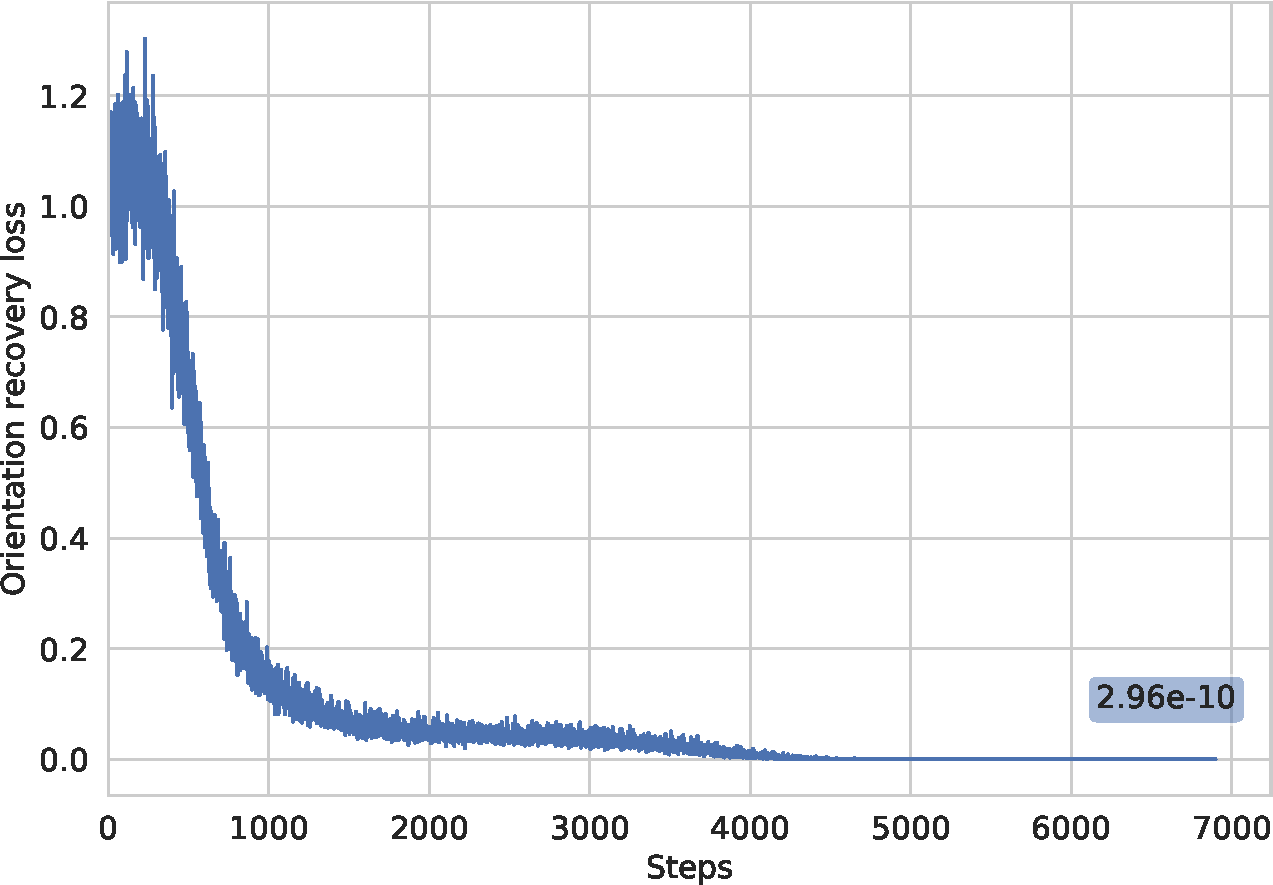
\includegraphics[height=3cm]{figures/5j0n_perfect_angle_recovery}
        % 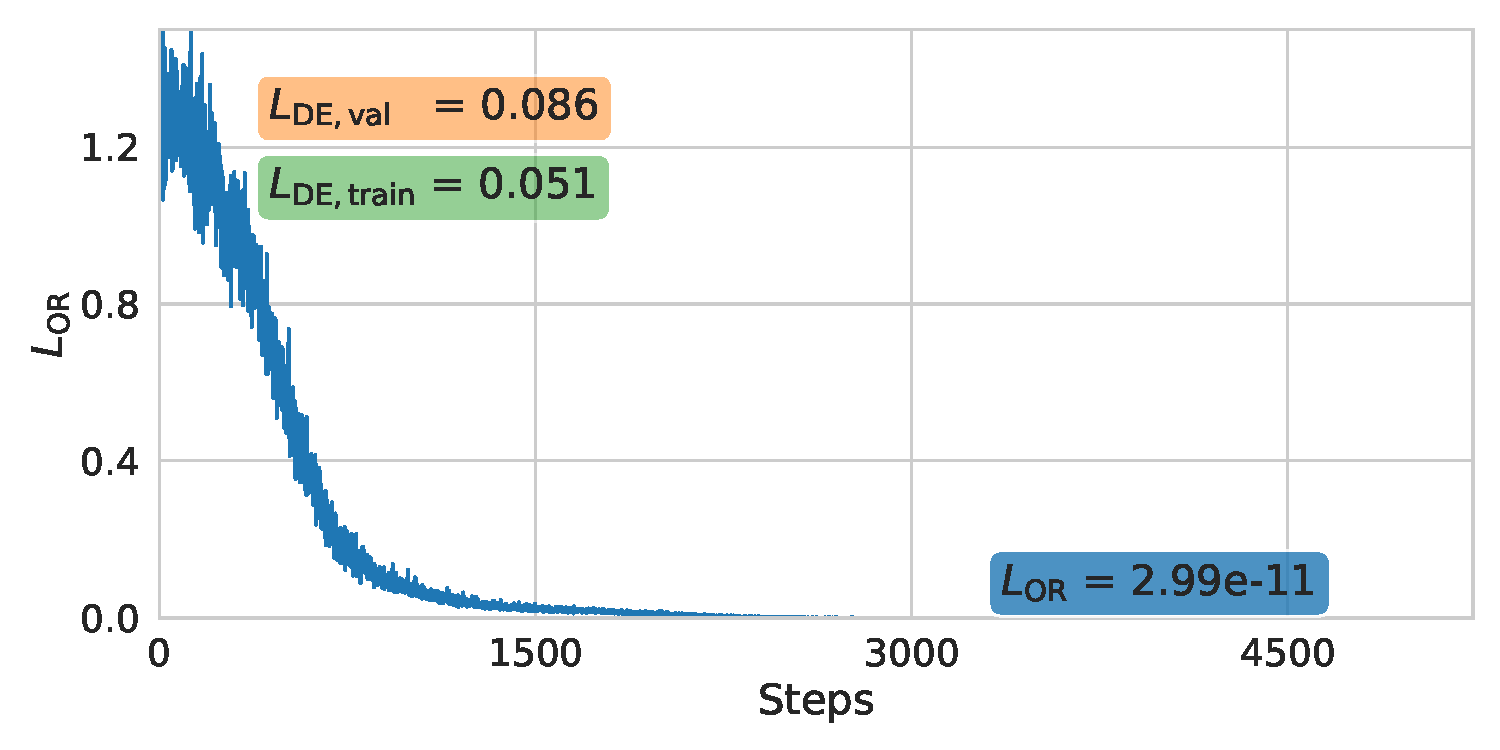
\includegraphics[height=3cm]{figures/5a1a_quartercov_uniformS2_halfInplane_ar_aa}
        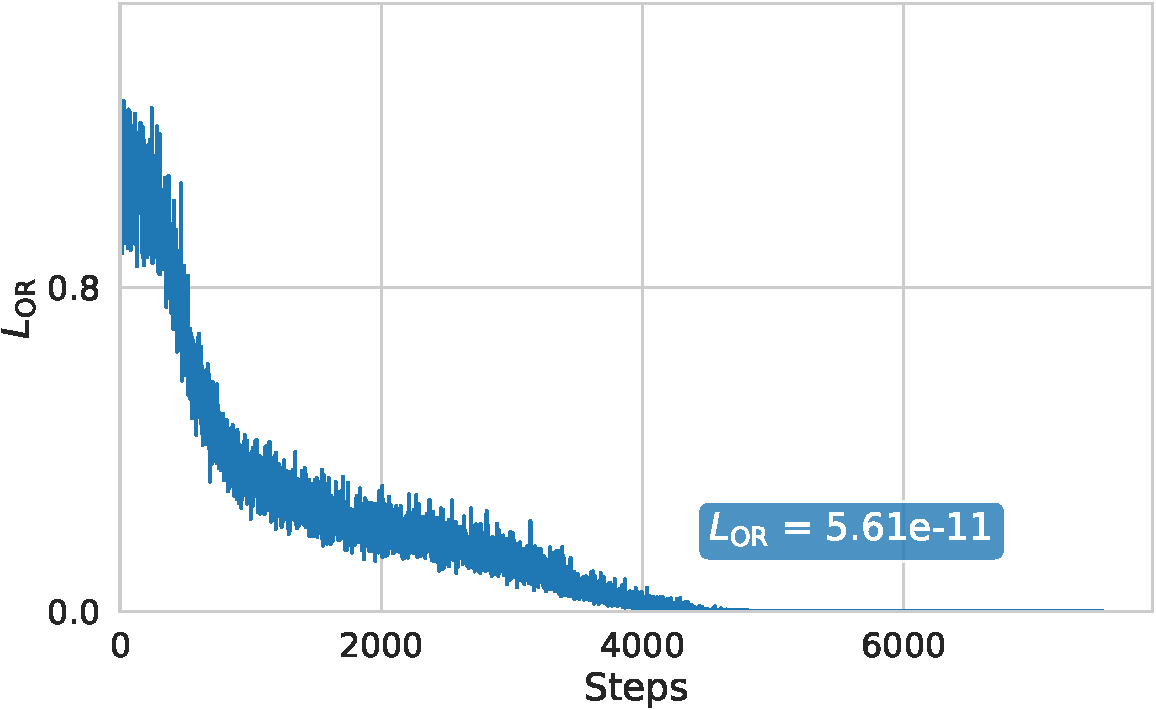
\includegraphics[height=3cm]{figures/5a1a_quartercov_uniformS2_perfect_ar_aa}
        \caption{%
            Example of perfect orientation recovery (for \texttt{5a1a}).
            The loss $L_\text{OR}$ \eqnref{orientation-recovery} converges to zero when the distance estimation is perfect, \ie, $\widehat{d_p}(\p_i, \p_j) = d_q(q_i, q_j)$.
            %\todo{Update to full in-plane.}
        }\label{fig:5j0n-orientation-recovery-loss}
    \end{minipage}
    \hfill
    \begin{minipage}[t]{0.66\linewidth}
%        \begin{subfigure}[b]{0.19\linewidth}
%            \centering
%            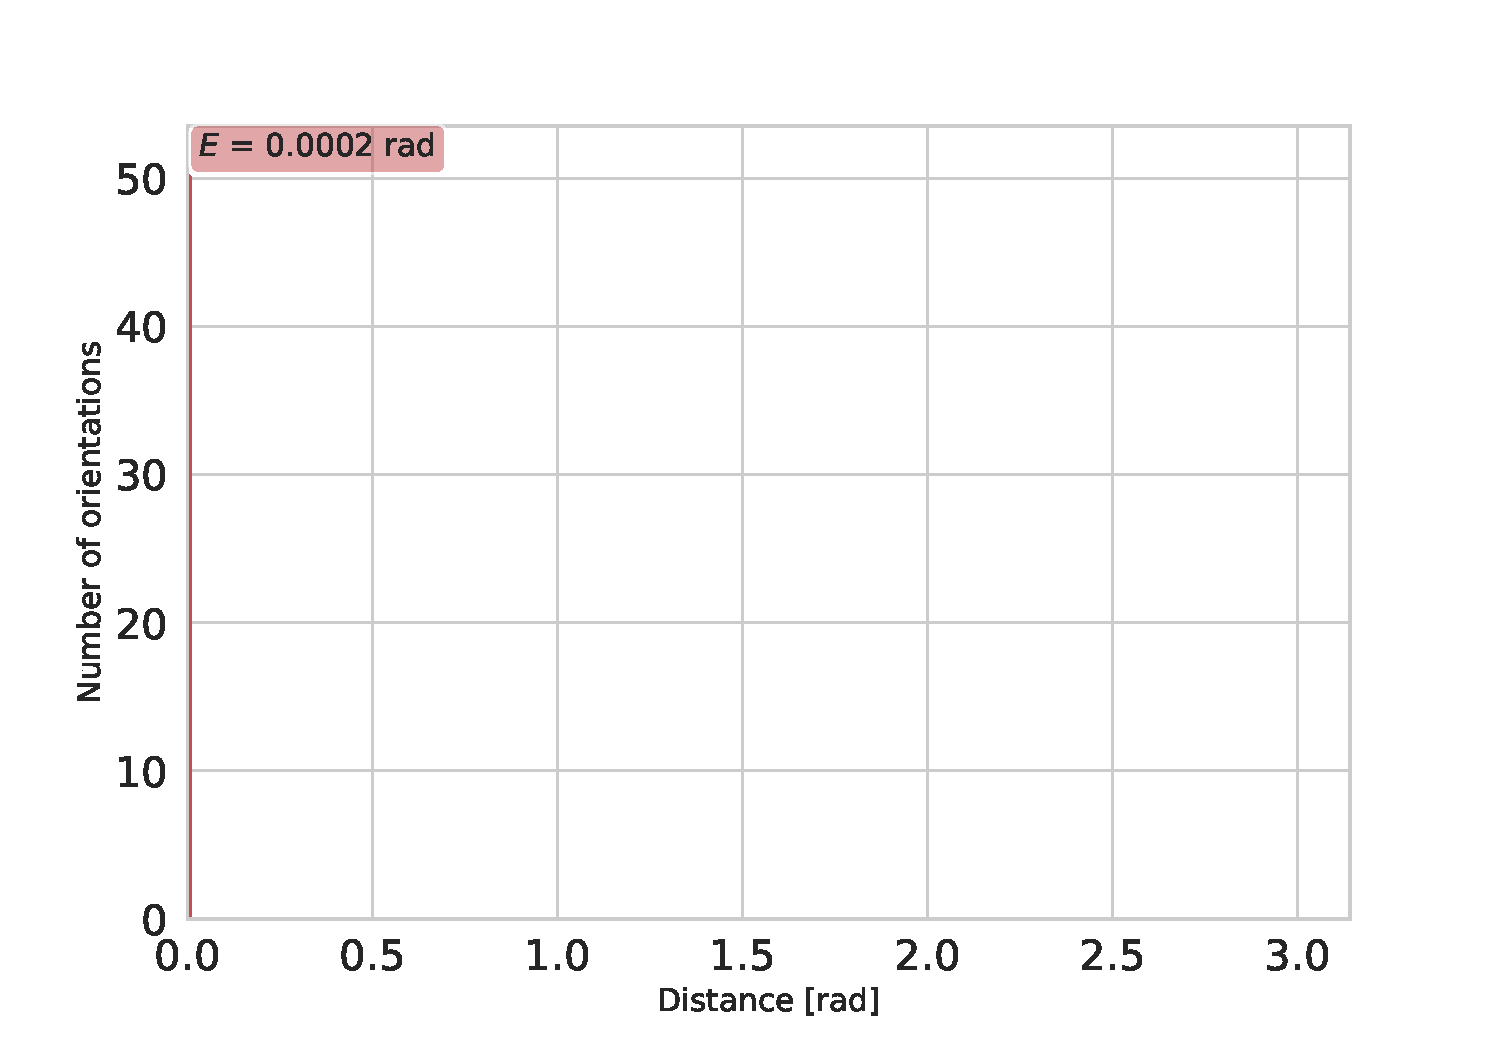
\includegraphics[height=3cm]{figures/5j0n_perfect_angle_ralignment_after}
%            \caption{Orientation recovery error with alignment.}
%        \end{subfigure}
%        \hfill
        % \begin{subfigure}[t]{4.3cm}
        %     \centering
        %     %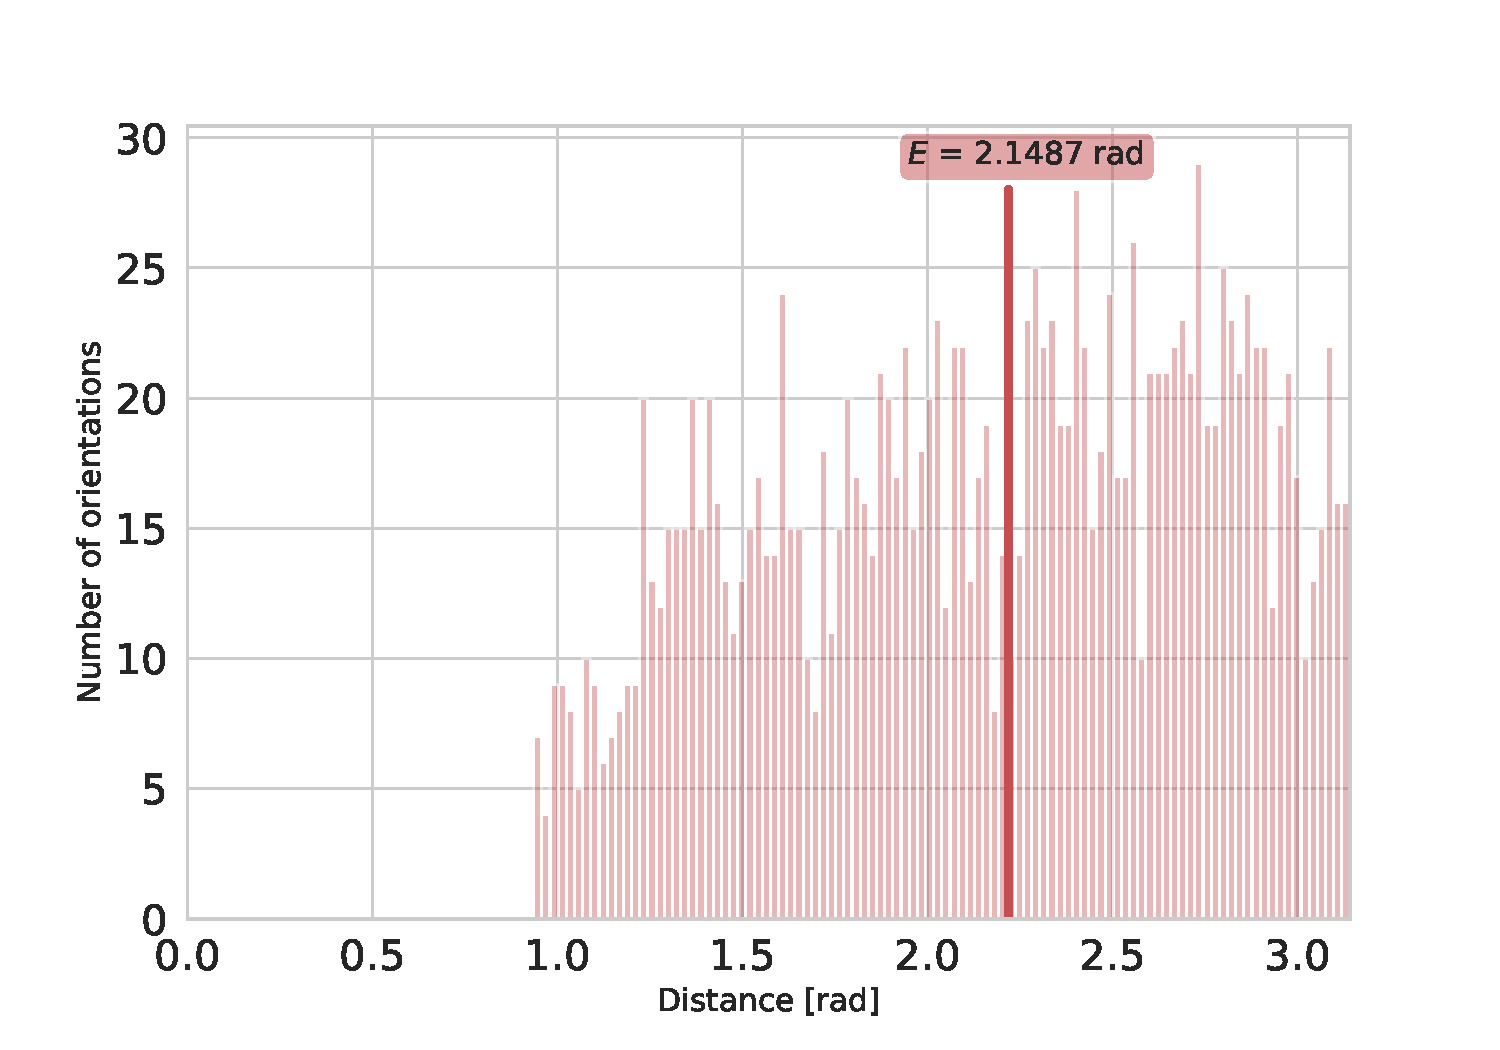
\includegraphics[height=3cm]{figures/5j0n_perfect_angle_ralignment_before}
        %     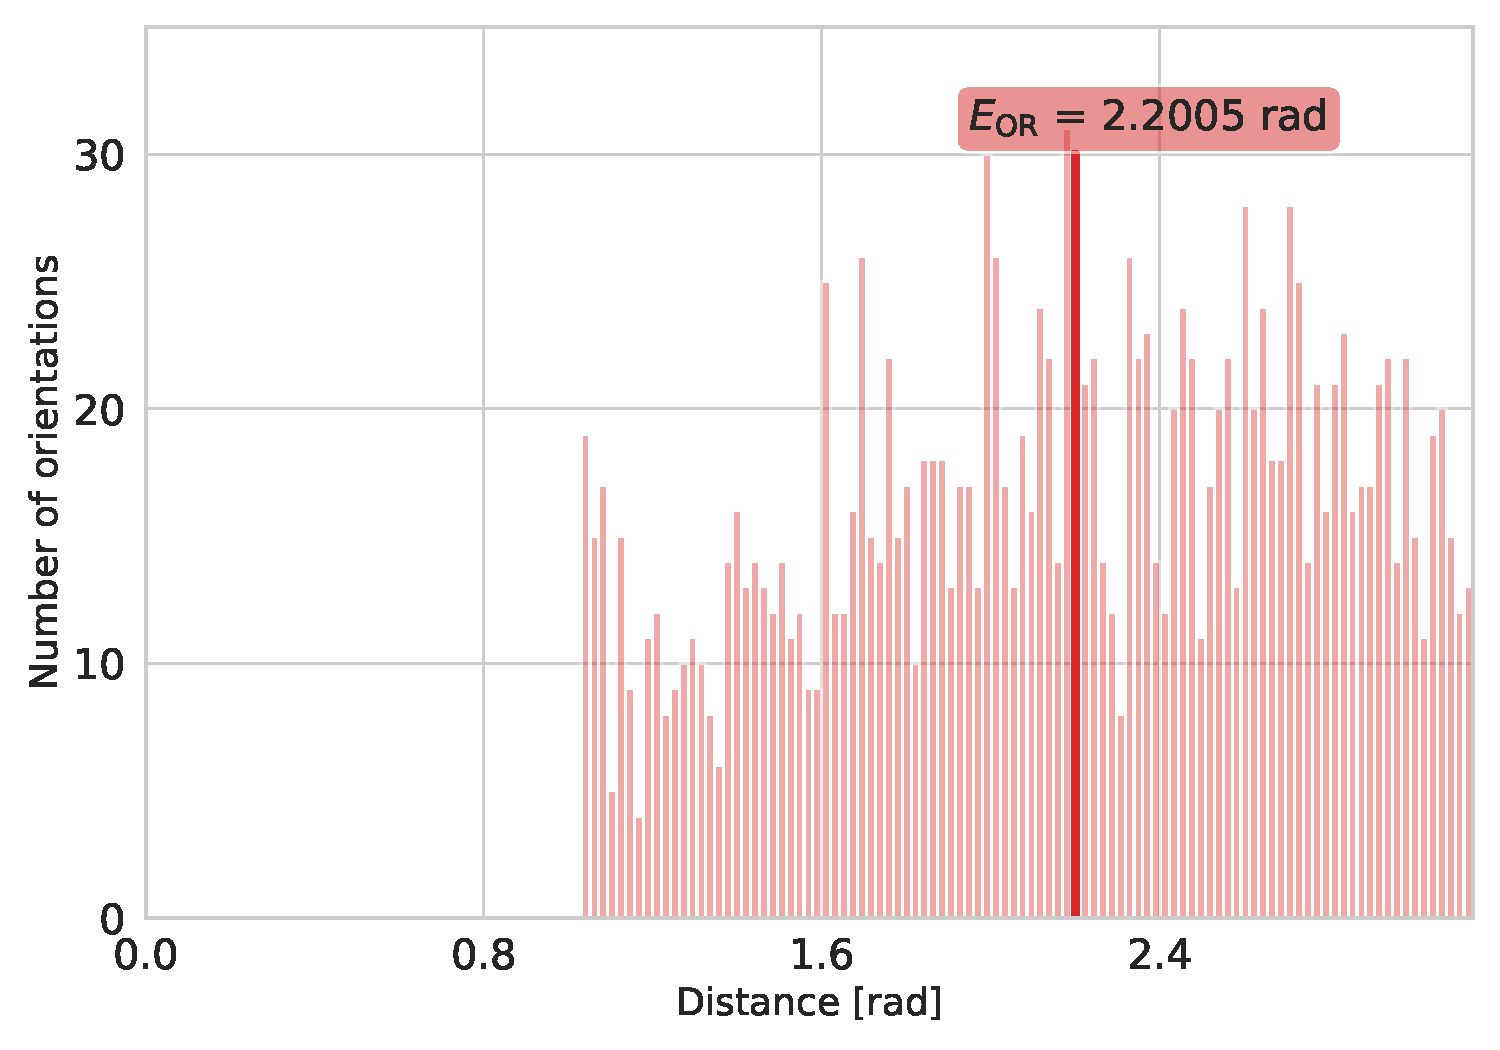
\includegraphics[height=3cm]{figures/5a1a_quartercov_uniformS2_halfInplane_before_alignment}
        %     \caption{Error histogram $\{ d_q (q_i, \widehat{q_i}) \}$, \ie, before alignment.}
        % \end{subfigure}
        % \hfill
        \begin{subfigure}[t]{0.49\linewidth}
            \centering
            % 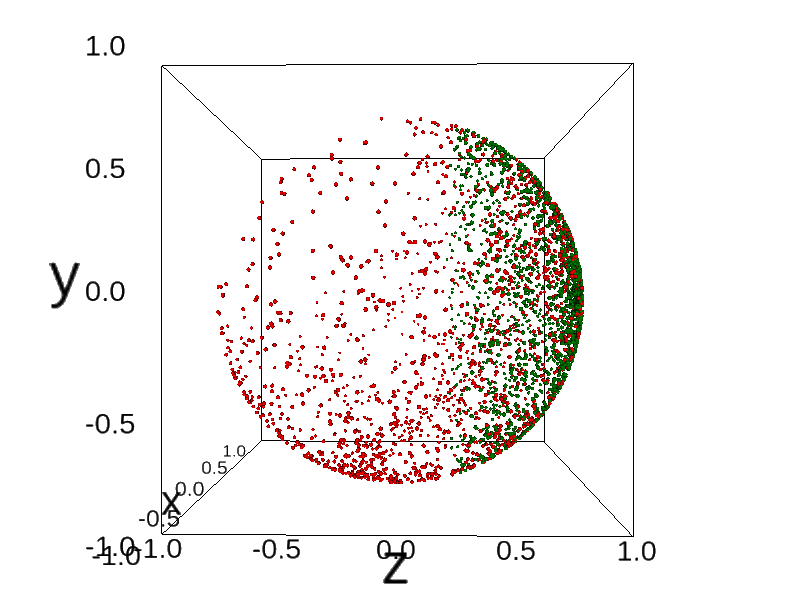
\includegraphics[height=3cm]{figures/coverage_alignment_before.png}
            %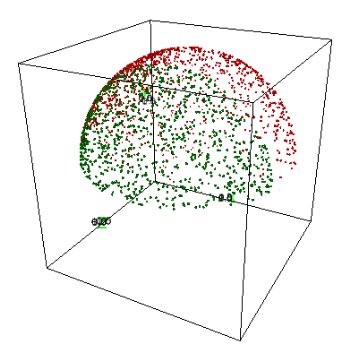
\includegraphics[height=3cm]{figures/before_aa.png}
            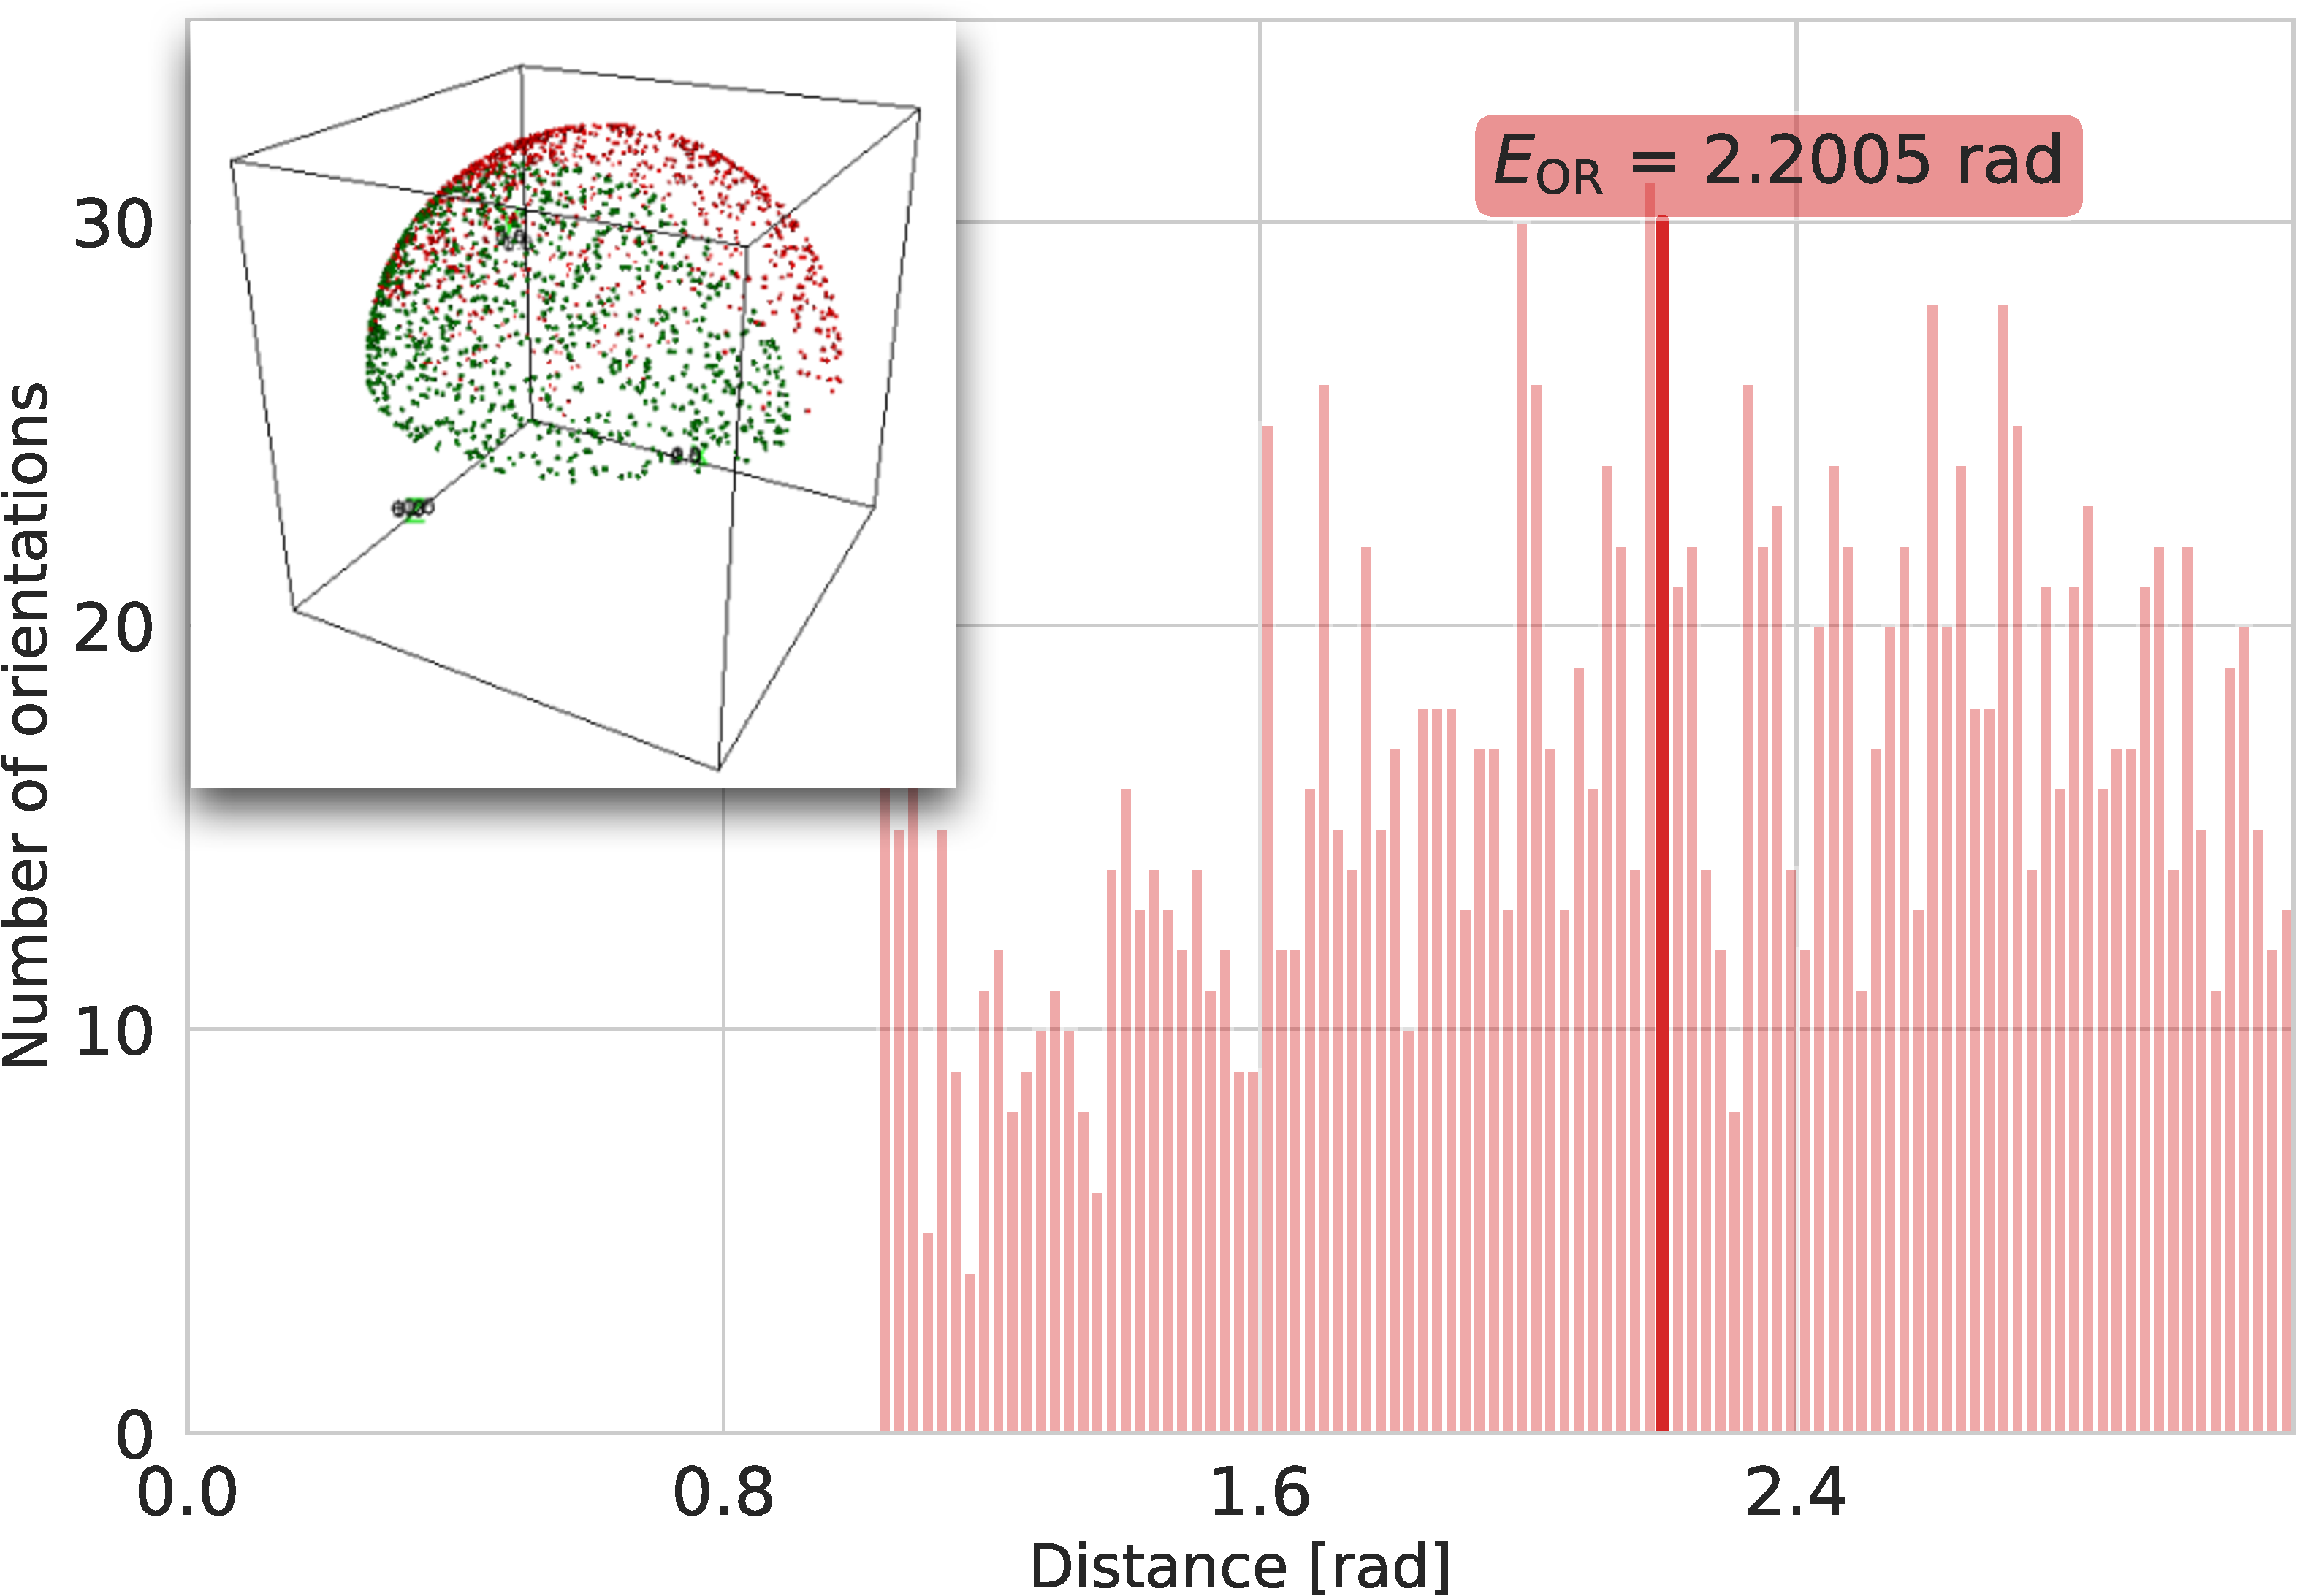
\includegraphics[height=3cm]{figures/BeforeAA.pdf}
            \caption{Orientations before alignment.}
        \end{subfigure}
        \hfill
        \begin{subfigure}[t]{0.49\linewidth}
            \centering
            % 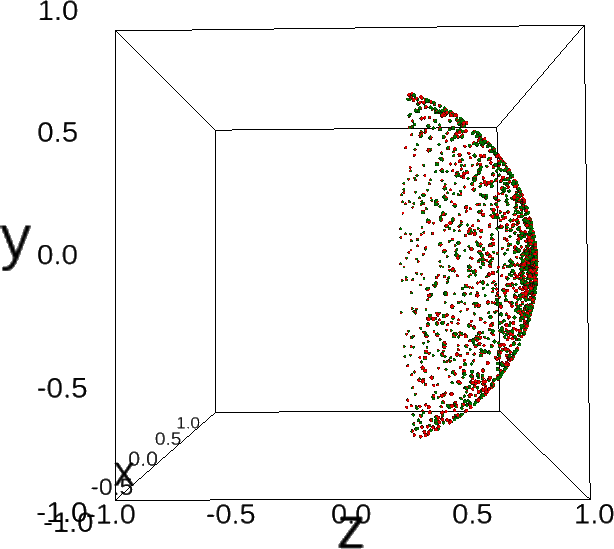
\includegraphics[height=3cm]{figures/coverage_alignment_after.png}
            %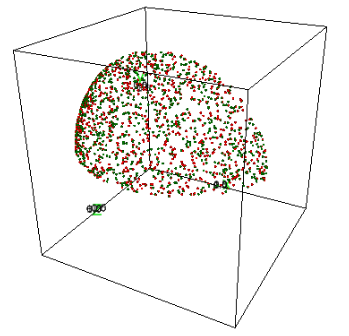
\includegraphics[height=3cm]{figures/after_aa.png}
            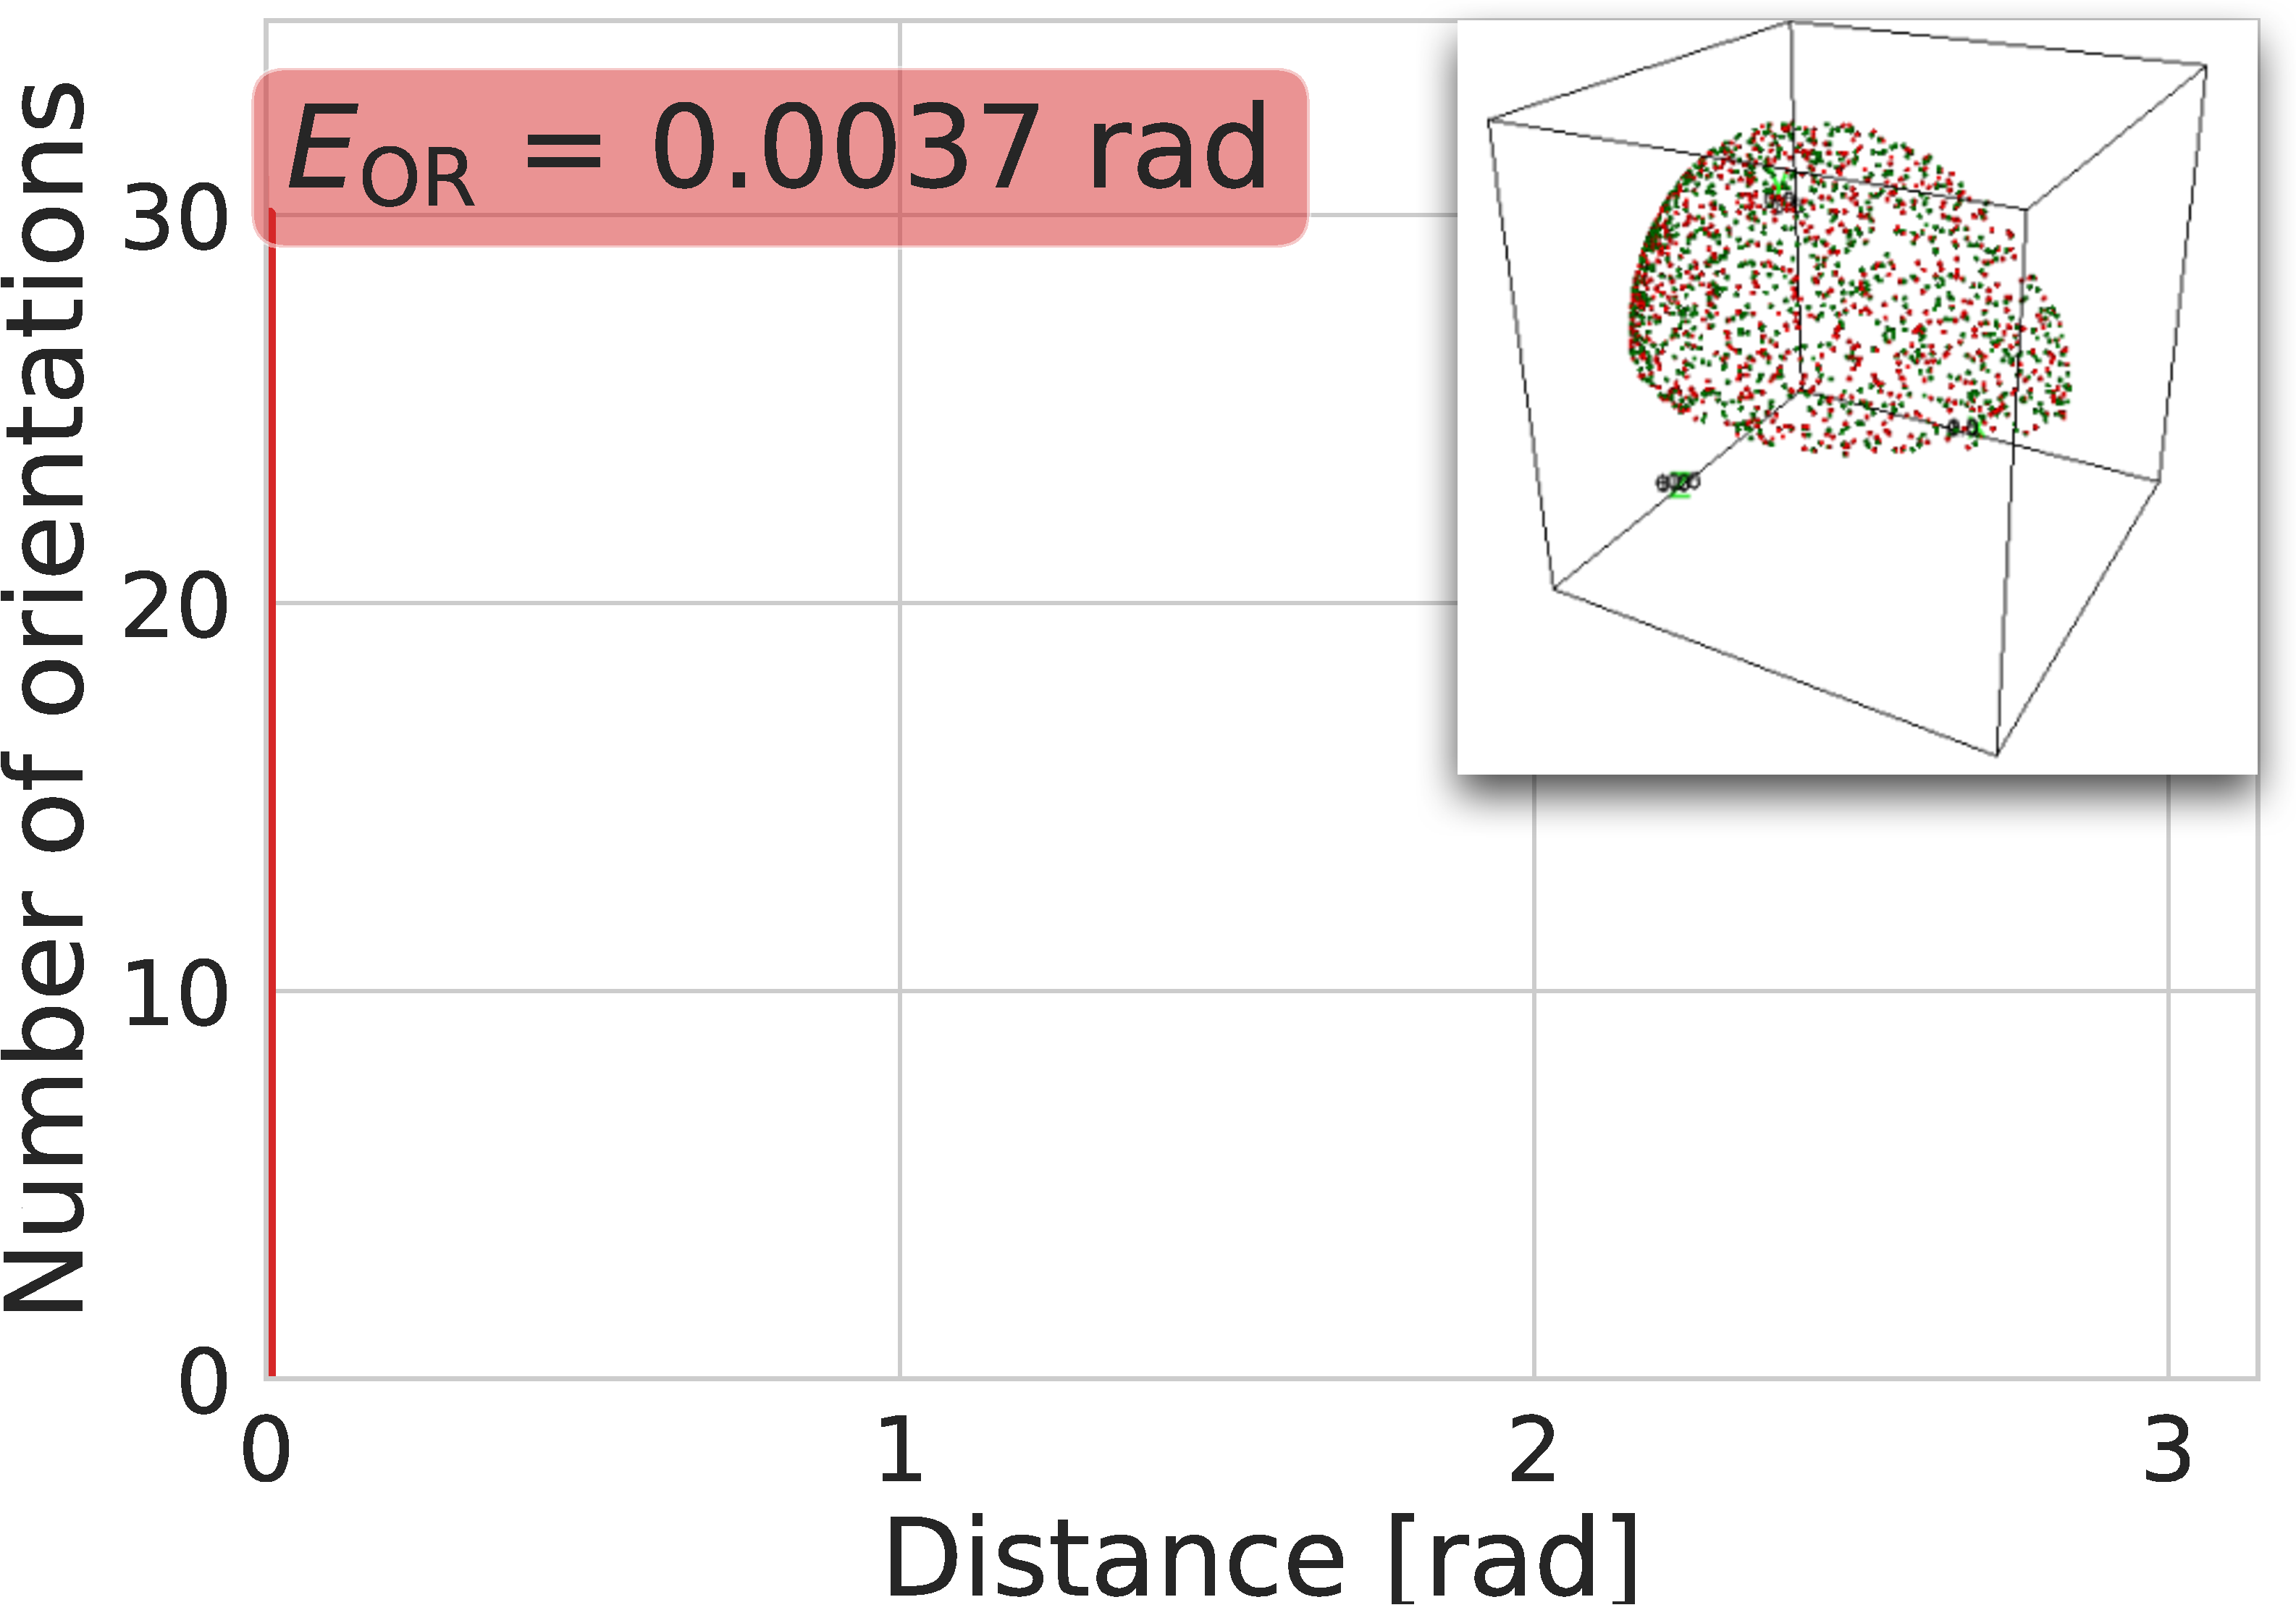
\includegraphics[height=3cm]{figures/AfterAA.pdf}
            \caption{Orientations after alignment.}
        \end{subfigure}
        \caption{%
            Example of perfect alignment~\eqnref{orientation-recovery-error} after a perfect orientation recovery~\eqnref{orientation-recovery}.
            The red histogram shows the errors in the recovered orientations  (a) $\{d_q(q_i, \widehat{q_i})\}$ and (b) $\{d_q(q_i, \T \widehat{q_i})\}$, with the mean $E_\text{OR}$ highlighted.
            % and $\T$ as the optimum of \eqnref{orientation-recovery-error} on the right.
            Directions $(\theta_2, \theta_1)$ are shown in the insert: Green points are the ground-truth orientations $\{q_i\}$ and red points are the recovered orientations $\{\widehat{q_i}\}$.
            While both colors are seen in (b), they are exactly superimposed.
        }\label{fig:5j0n-aa-loss-perfect-distances}
    %    \label{fig:angle-alignment-perfect}
    \end{minipage}
\end{figure}

\section{Euclidean distance between projections}\label{apx:results:distance-estimation:euclidean}

%\mdeff{Story: simplest baseline estimator, $d_{pe}$ somewhat estimates $d_q$, quickly plateaus (even in the simplest noiseless and centered case).
%Note the difference between symmetric and asymmetric proteins.}

We evaluate $\widehat{d_p}(\p_i, \p_j) = \| \p_i - \p_j \|_2$ (\ie, the Euclidean distance) as a baseline distance estimator.
\figref{euclidean-not-robust} shows the relationship between $\widehat{d_p}$ and $d_q$.
Two main observations can be made from this experiment.
First, as suspected, $d_p$ fails to be a consistent predictor of $d_q$, even in the simple imaging conditions considered here (no noise, no shift, no PSF).
In particular, the larger the orientation distance $d_q$, the poorer the predictive ability of $d_p$ (the plot plateaus).
Second, because \texttt{5a1a} has D2 symmetries, two projections might be identical while not having been acquired from the same orientation.
Restricting directions to a quarter capture only one of four identical projections, solving the issue.

\begin{figure}
    \begin{minipage}[t]{0.99\linewidth}
        \begin{subfigure}[t]{0.33\textwidth}
            \centering
            %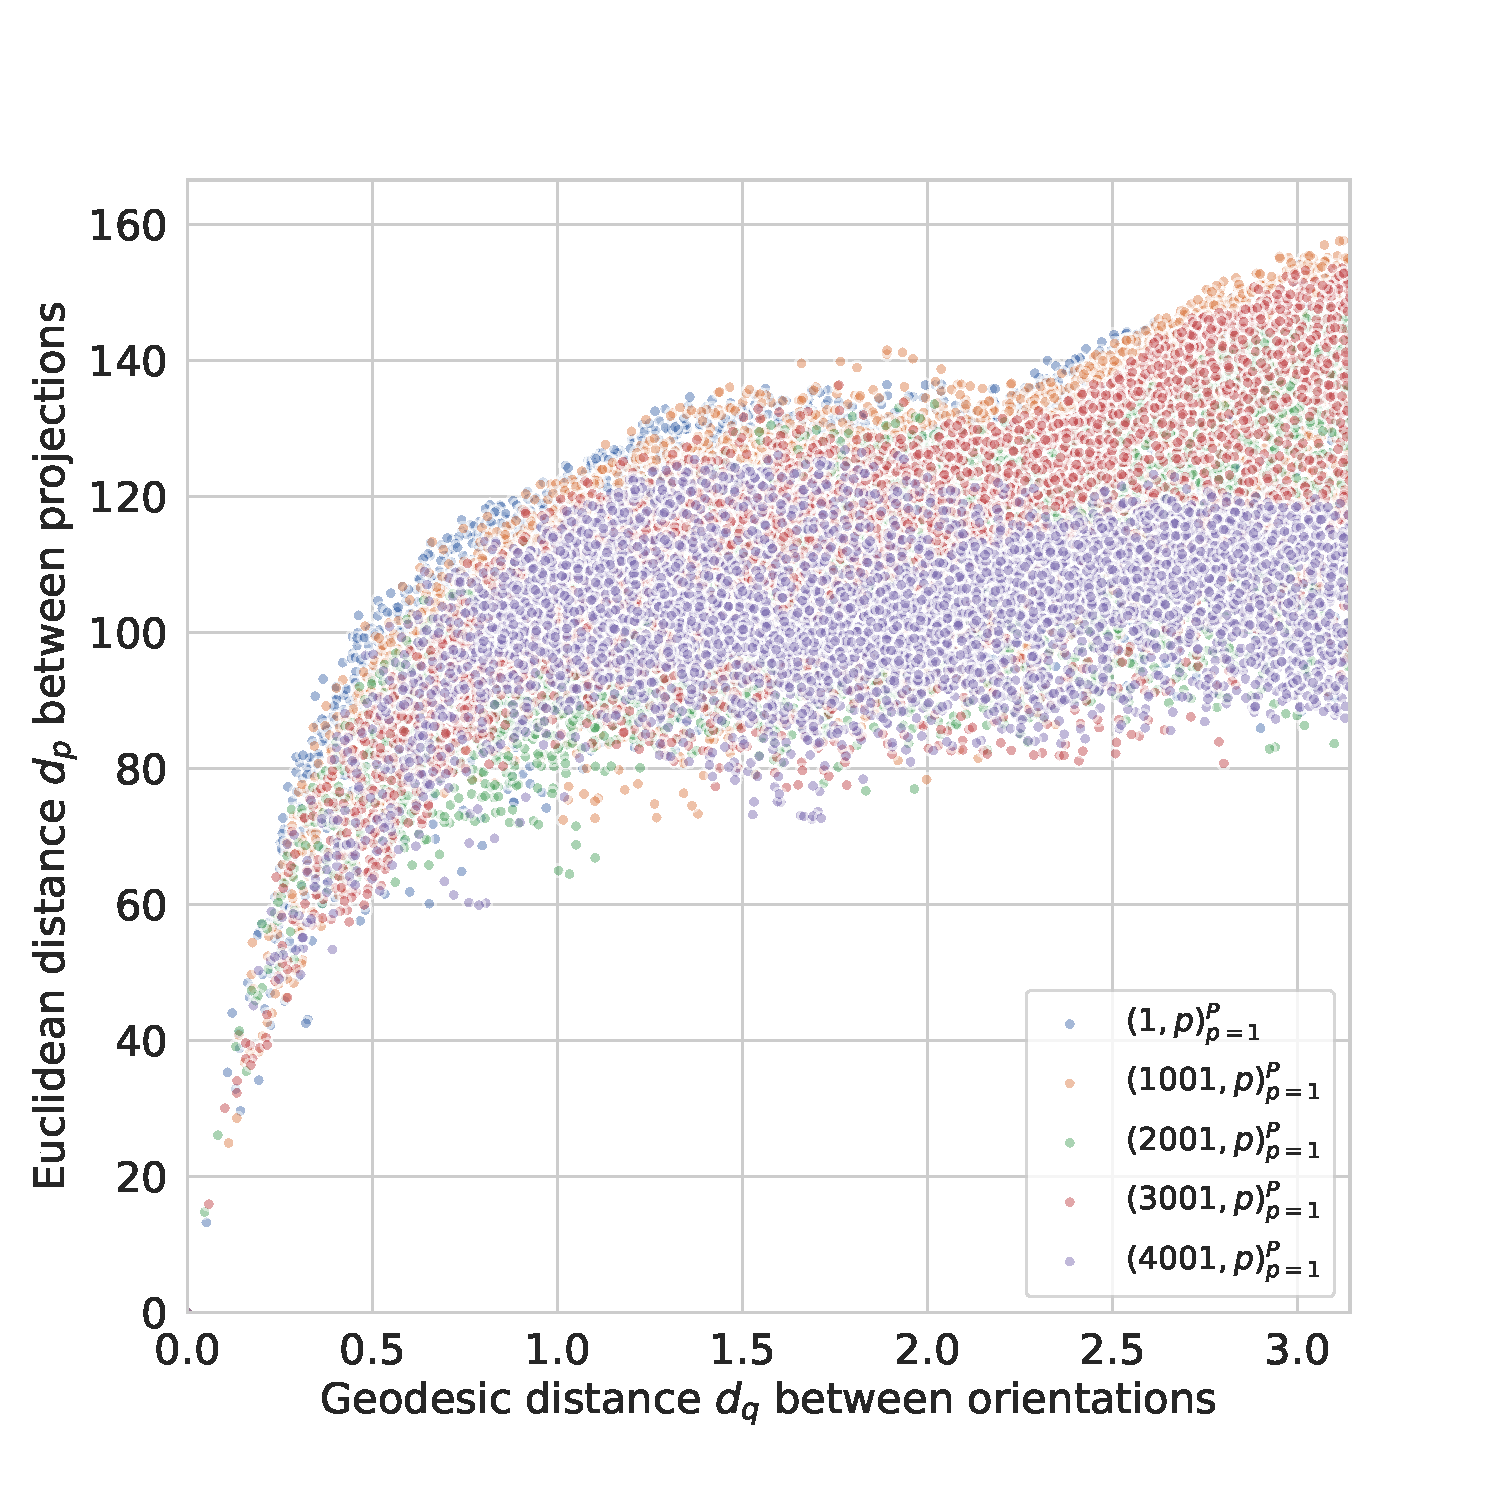
\includegraphics[height=4cm]{figures/eucl_notrobust_5j0n}   % on half-sphere
            %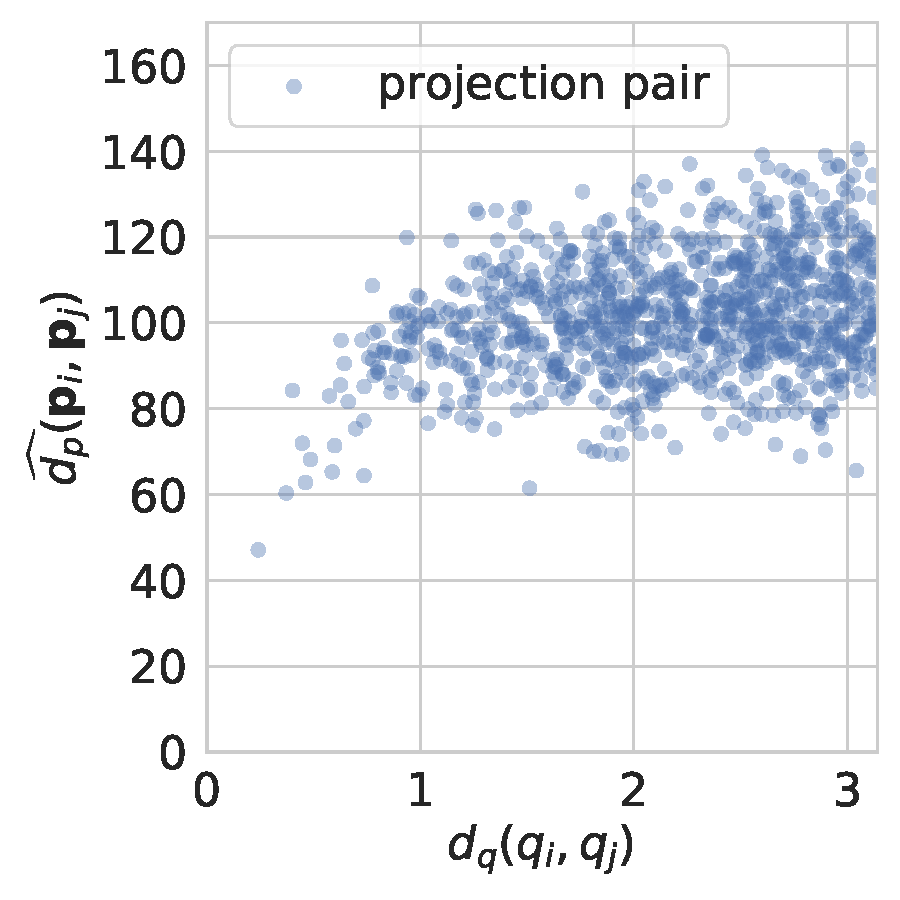
\includegraphics[height=4cm]{figures/dPdQ_5j0n_euclidean}
            % 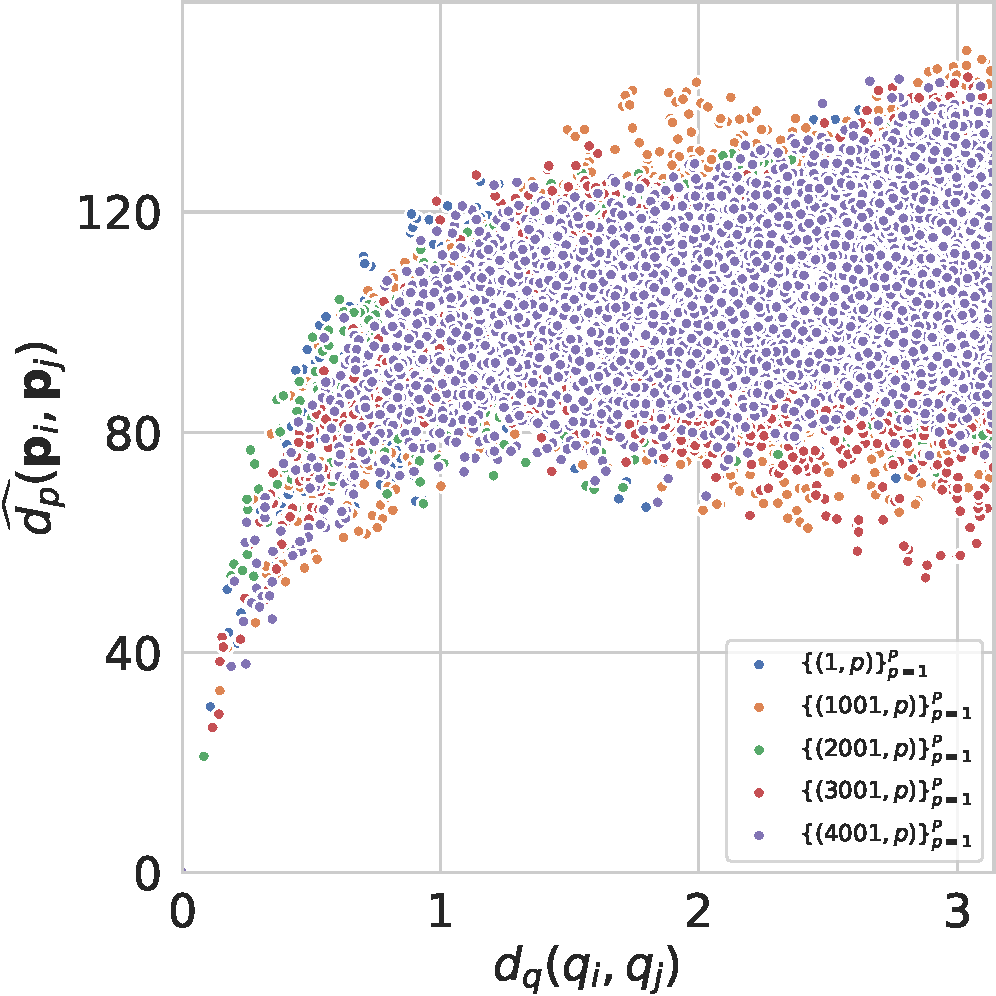
\includegraphics[height=3cm]{figures/dPdQ_5j0n_euclidean2.pdf}
            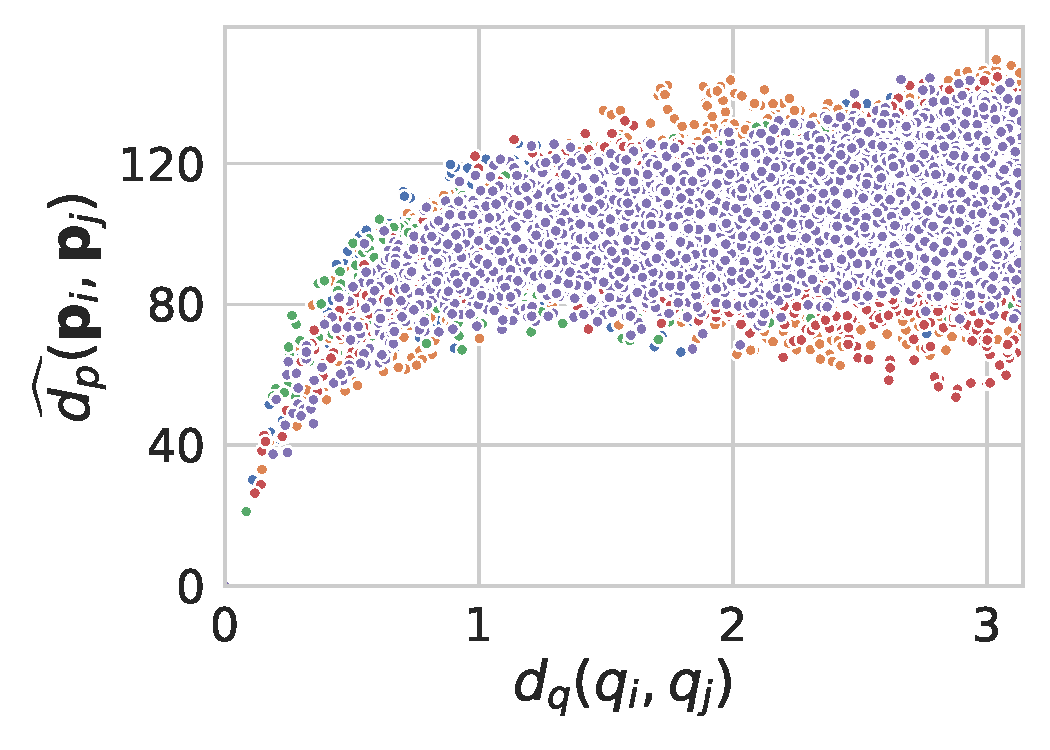
\includegraphics[height=3cm]{figures/dPdQ_5j0n_euclidean3.pdf}
            \caption{Full direction coverage on \texttt{5j0n}.}%
            \label{fig:euclidean-not-robust:5j0n-full}
        \end{subfigure}
        \hfill
        \begin{subfigure}[t]{0.33\textwidth}
            \centering
            % 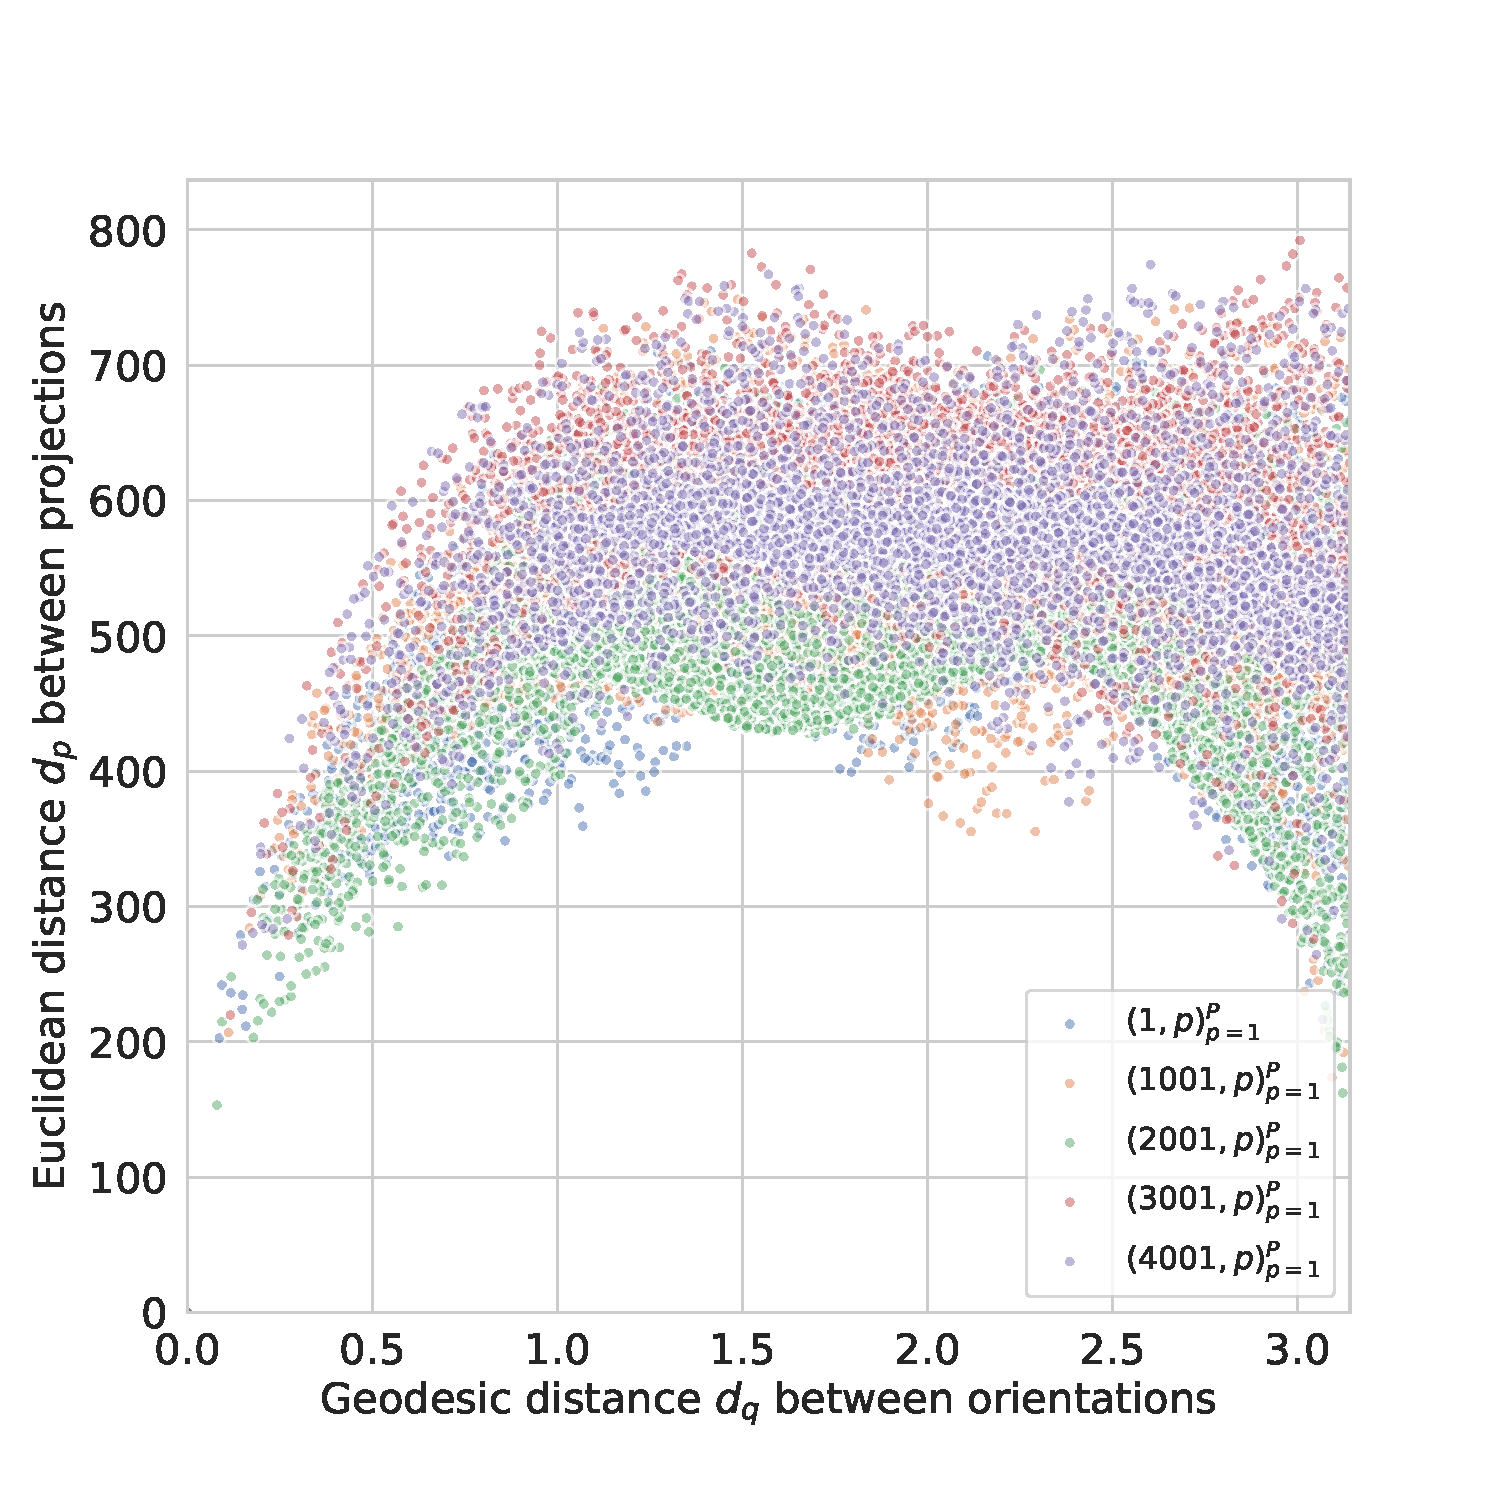
\includegraphics[height=4cm]{figures/eucl_notrobust_5a1a}
            % 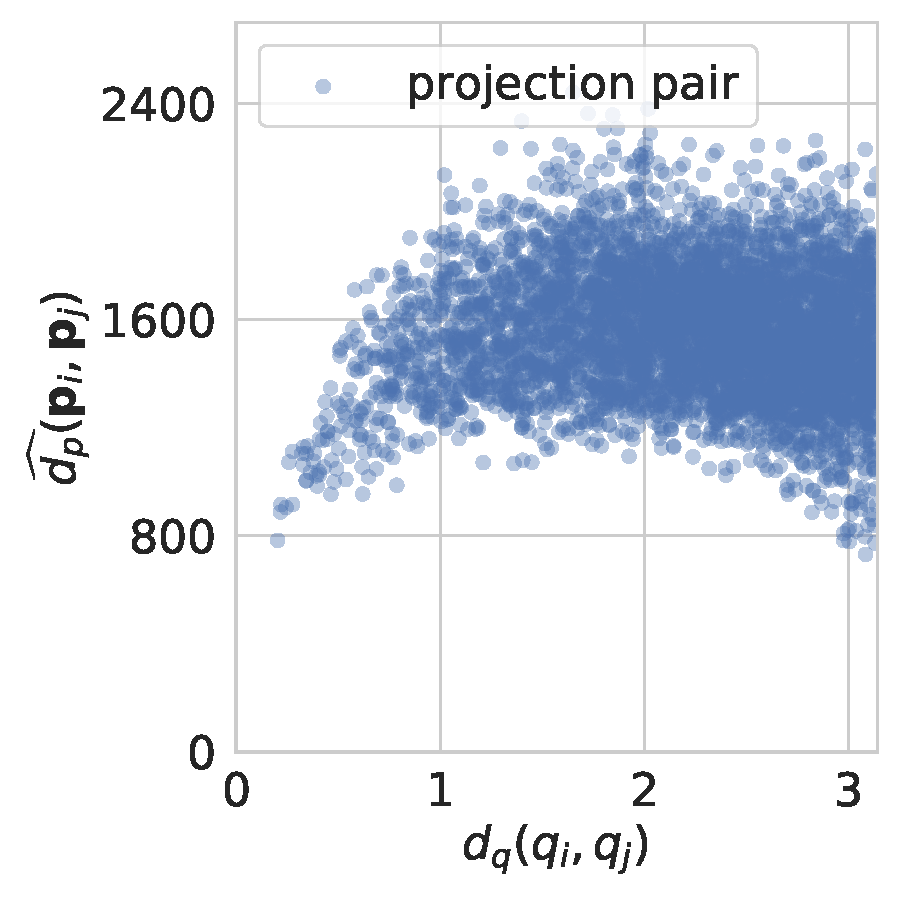
\includegraphics[height=4cm]{figures/dPdQ_5a1a_full_euclidean}
            % 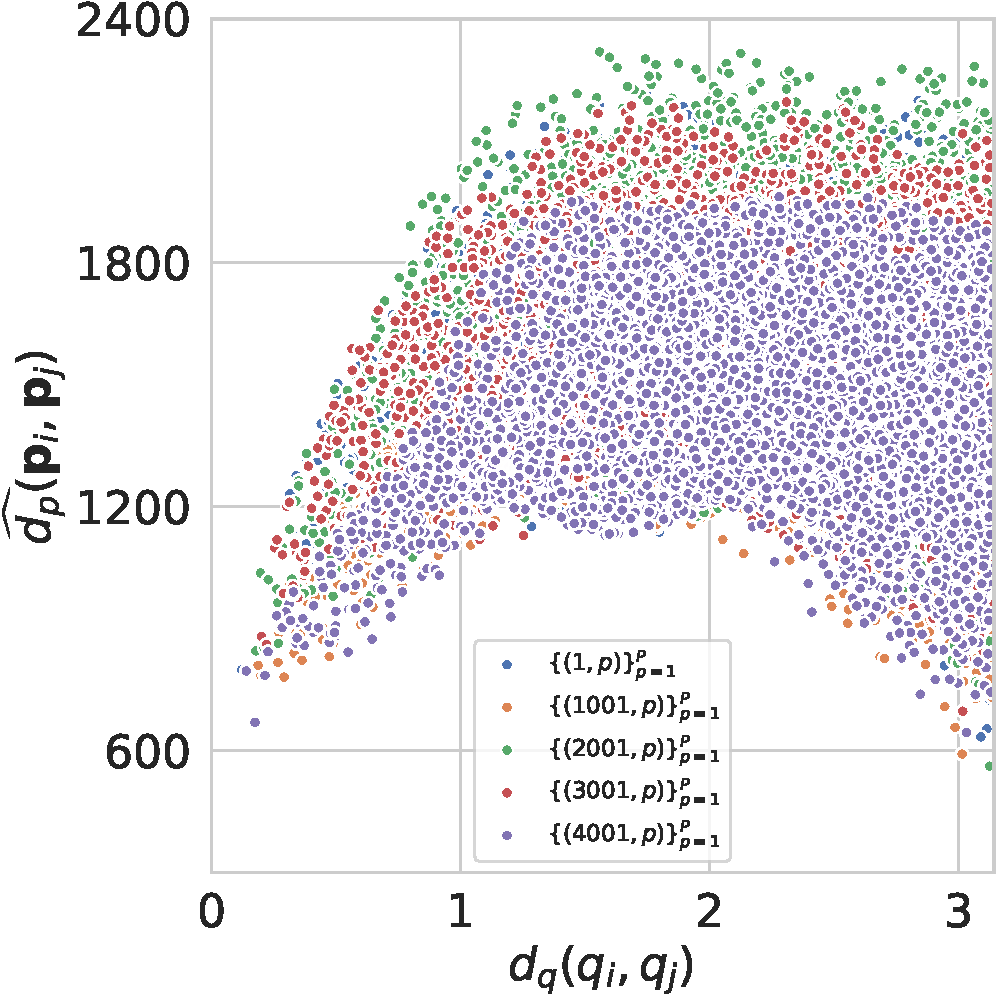
\includegraphics[height=3cm]{figures/dPdQ_5a1a_full_euclidean2.pdf}
            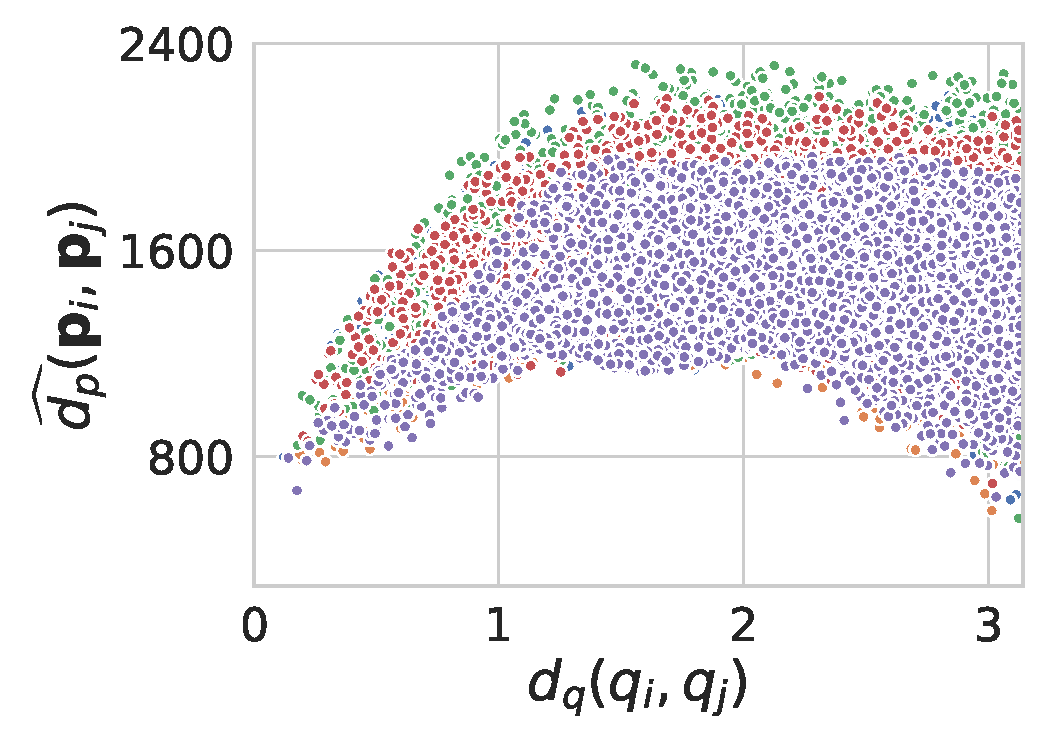
\includegraphics[height=3cm]{figures/dPdQ_5a1a_full_euclidean3.pdf}
            \caption{Full direction coverage on \texttt{5a1a}.}%
            \label{fig:euclidean-not-robust:5a1a-full}
        \end{subfigure}
        \hfill
        \begin{subfigure}[t]{0.33\textwidth}
            \centering
            %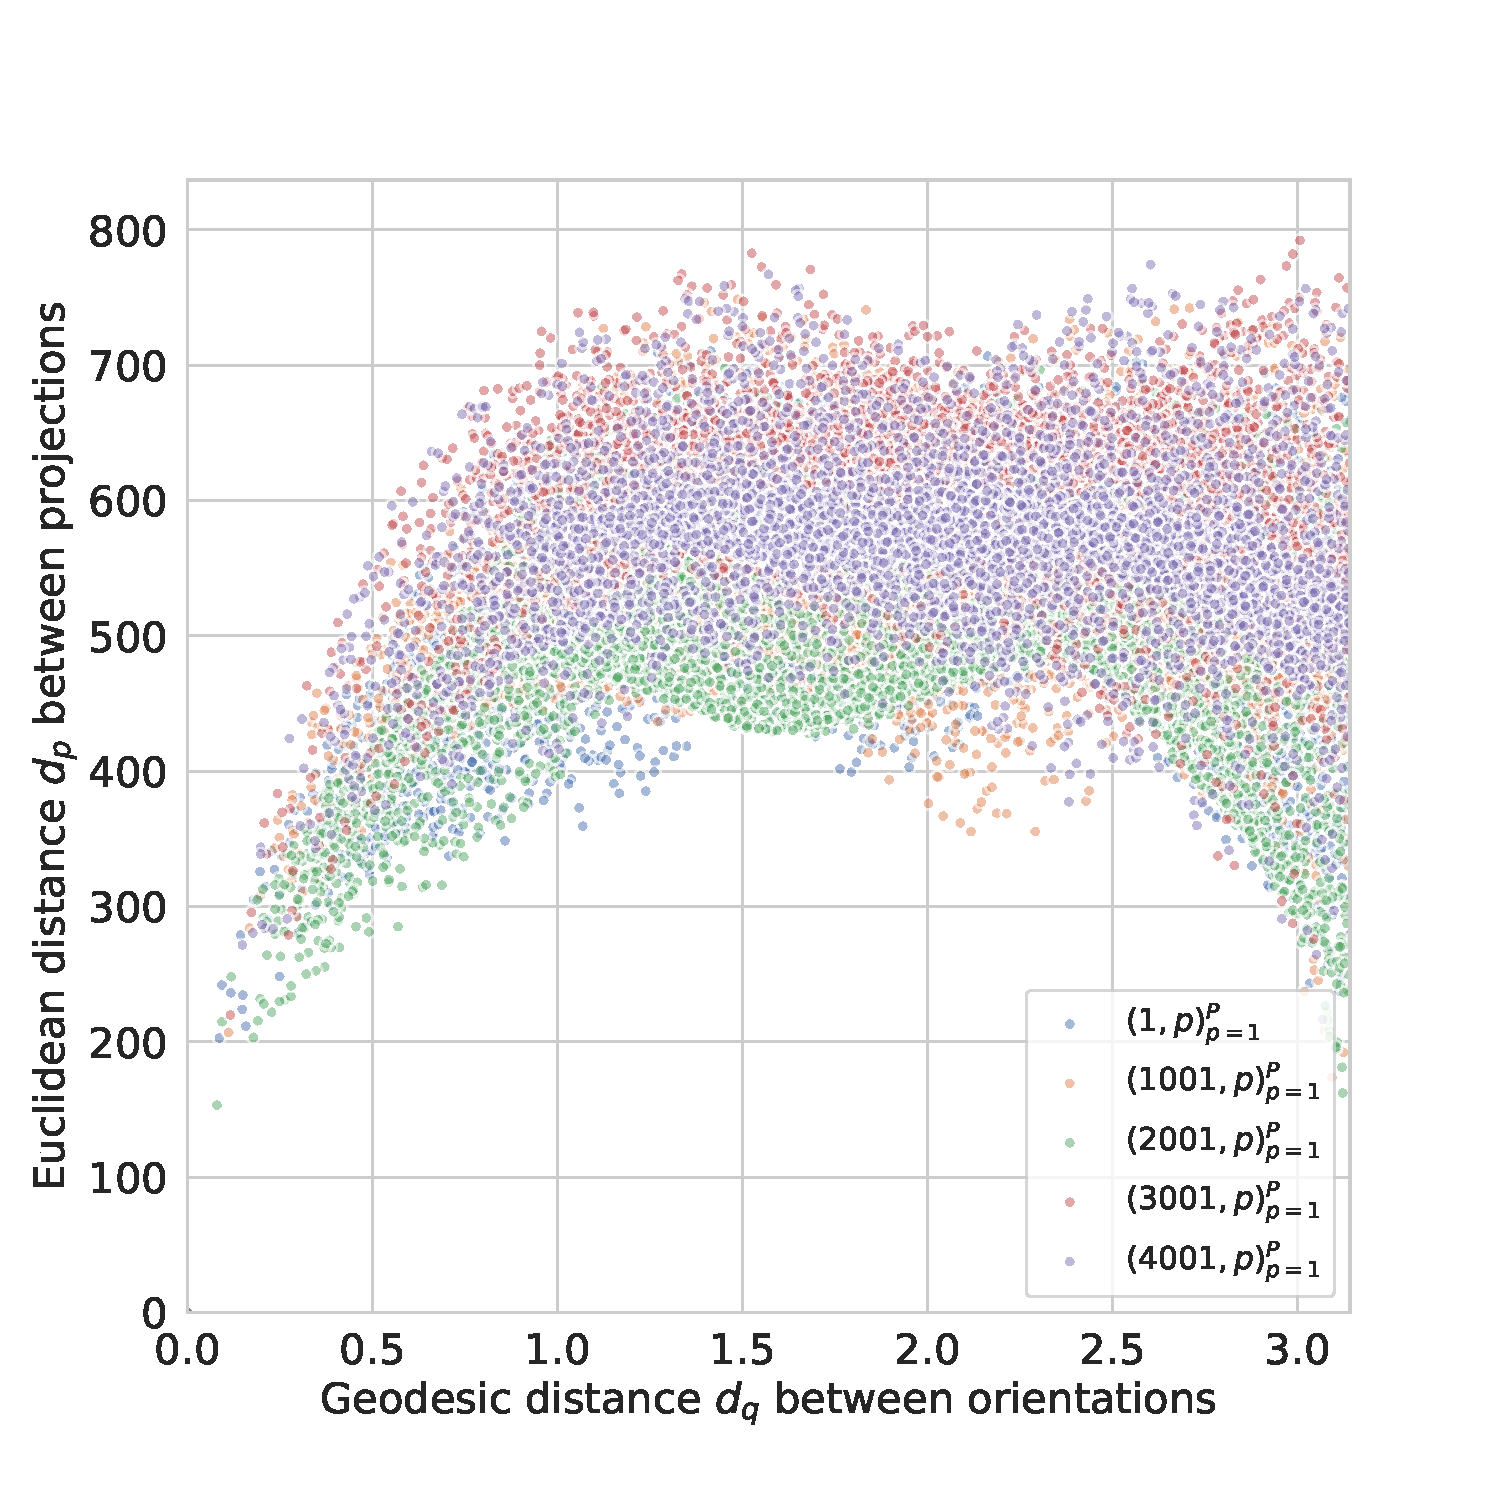
\includegraphics[height=4cm]{figures/eucl_notrobust_5a1a}  % on half-sphere
            %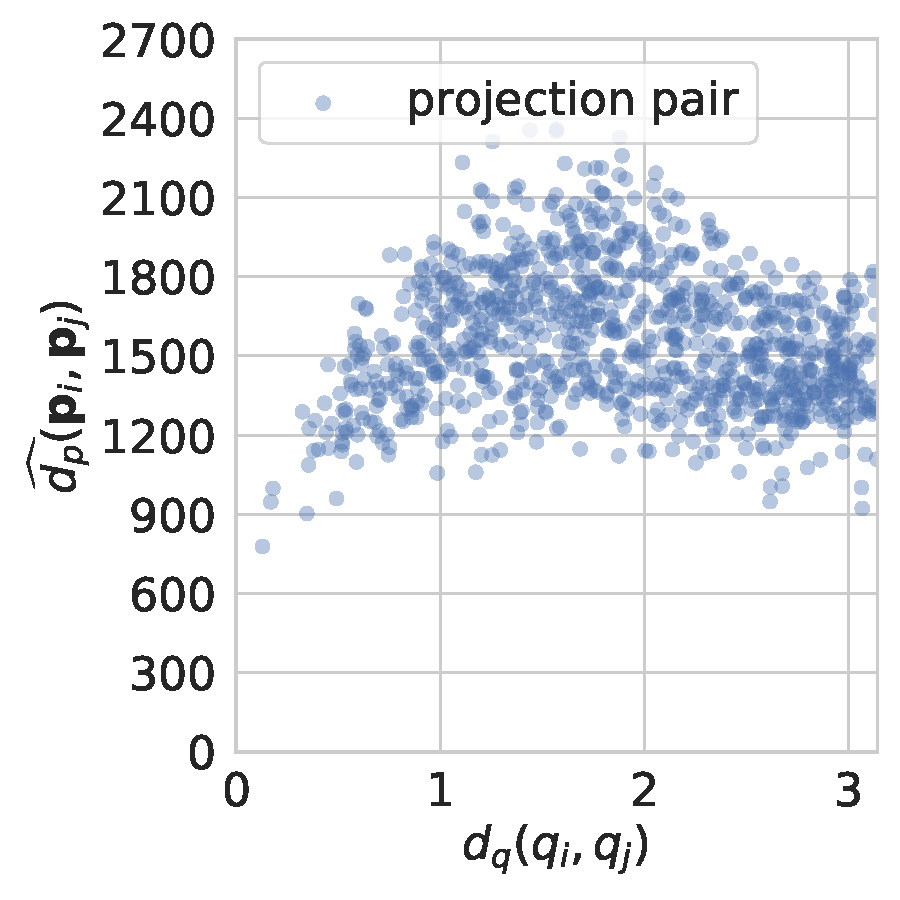
\includegraphics[height=4cm]{figures/dPdQ_5a1a_euclidean}
            % 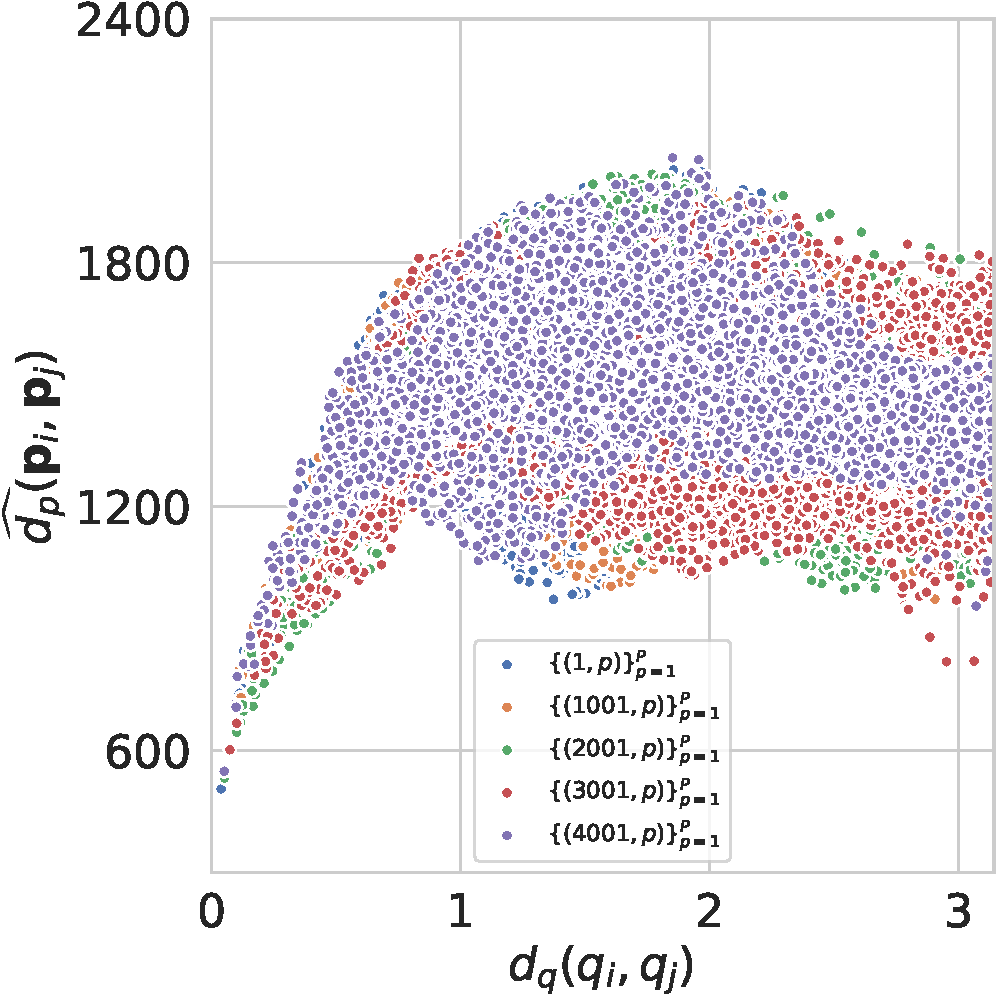
\includegraphics[height=3cm]{figures/dPdQ_5a1a_euclidean2.pdf}
            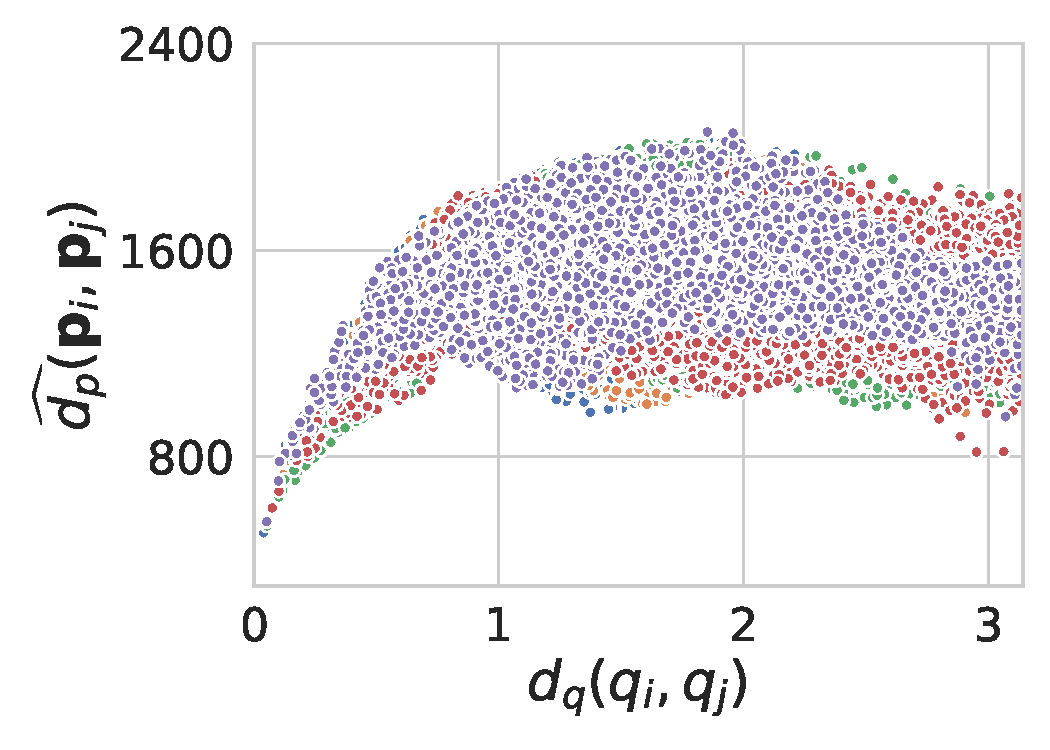
\includegraphics[height=3cm]{figures/dPdQ_5a1a_euclidean3.pdf}
            \caption{Quarter direction coverage on \texttt{5a1a}.}%
            \label{fig:euclidean-not-robust:5a1a-quarter}
        \end{subfigure}
        \caption{%
            Euclidean distance between projections $\widehat{d_p}(\p_i, \p_j) = \| \p_i - \p_j \|_2$ versus their actual relative orientation $d_q(q_i, q_j)$.
            From $P = 5,000$ possible projection, we randomly selected $5$ projections.
            Each color represent the distances between one fixed projection and the other $P-1$ projections.
    %        The color corresponds to projection pairs that share one projection, \ie, distance between one projection with all other projections.
            % \todo{Make the plots flatter. Larger text. Remove the legend (we explain it and it's two small anyway).}
        }\label{fig:euclidean-not-robust}
    \end{minipage}
\end{figure}


% \section{Estimating distances on unseen proteins}\label{apx:unseen-proteins}
% %\section{Non-determinism of the Orientation Recovery}\label{apx:non-determinism}

% As the SiameseNN will ultimately be trained on known proteins and used to estimate distances on unknown proteins to be imaged,
% %we also desire our learned distance function to generalize/transfer across density maps $\x$.
% we also desire our learned distance function to generalize to unseen proteins.
% The distance function $\widehat{d_p}$ must abstract the protein---in the same way it must abstract shifts, noise, or PSFs to generalize to unseen projections.
% We attempted to recover the orientations of noiseless projections from \texttt{5j0n} while we had trained the SiameseNN on $4,000$ noiseless projections from four other proteins (\texttt{5nvu}~\cite{ZHANG20171303}, \texttt{5nvs}~\cite{ZHANG20171303}, \texttt{6mem}~\cite{iwai2018unique}, \texttt{6o1o}~\cite{liu2019target}, which have the same type of symmetry as \texttt{5j0n}).
% \mdeff{The type of symmetry shouldn't play a role.}
% \mdeff{But the resolution might. Do all the density maps have a resolution of 3.67\AA\@? What are the projection's size? $116 \times 116$?}
% %In this experiment, we generated $1,000$ projections per protein.
% %\todo{should be the same ``kind'' of refs as the ones used in 3.1 for \texttt{5j0n} and \texttt{5a1a}}
% %Four proteins were used in the training and validation set to ensure the robustness to the unseen protein \texttt{5j0n} used in the testing set.
% % %The number of projections in every set is the same as in \tabref{dataset}.
% We obtained a recovery loss of \todo{$L_\text{OR} = 0.014$},
% to be compared with \todo{$L_\text{OR} \approx 0.066$} when the SiameseNN was trained on \texttt{5j0n} alone.
% \mdeff{Weird that $L_\text{OR}$ is lower. Maybe OR finds a set of orientations that satisfy well the distances, though I can't understand how (it's not degenerated right?). Then bad distances -> bad orientations -> AA fails. If that's the case we should be careful about how we report it in \secref{discussion}.}
% \mdeff{What happens if we train with \texttt{5j0n} too? E.g., \texttt{5j0n} + 1/2/4 others. That should work.}
% \todo{While performance is somewhat degraded, we conclude that it is possible to train and use a distance function on different proteins.}

% \todo{Distance learning and orientation recovery worked well, but alignment didn't.}
% \mdeff{Why is dPdQ so bad? Seems contradictory to a low $L_\text{DE}$ and $L_\text{OR}$. Maybe that's why alignment didn't work? But then I don't get why $L_\text{DE}$ and $L_\text{OR}$ are so low\ldots.}
% \banjac{I don't know why it is bad, but the result of alignment visualized in the rotation vector space looks the same as for other cases we were not able to align. It seems the same transformation is missing...}

% \mdeff{Could we also have $E_\text{OR}$? It's easier to understand and compare.}
% \banjac{I fully agree, however, I already mentioned that I wasn't able to align the orientations even though the $L_\text{OR}$ was very good. Looking at the estimation and GT in rotation space, it is visible we have some kind of transformation between these two (transformation similar to one we found the flip is causing, but it is not the flip).}
% \mdeff{Could we show the ground-truth and estimated orientations in \figref{robustness-to-unseen-pipeline}?}
% \banjac{Visualized on the sphere - Coverage?}
% \mdeff{Coverage or rotation-vector, whichever you think best illustrate the non-alignment issue.}

% While alignment is in principle only necessary to compute $E_\text{OR}$, for an unknown reason, we had to align the recovered orientations with \eqnref{orientation-recovery-error} before feeding them to ASTRA\@.
% \banjac{Hypothesis: I think ASTRA tools for reconstruction have one coordinate system and our protein is reconstructed in another. The alignment that we do as a last step of the pipeline is actually the alignment to ASTRA coordinate system. I am not sure if modifying}

% \begin{figure}[ht!]
%     \centering
%     \begin{subfigure}[t]{0.32\linewidth}
%         \centering
%         %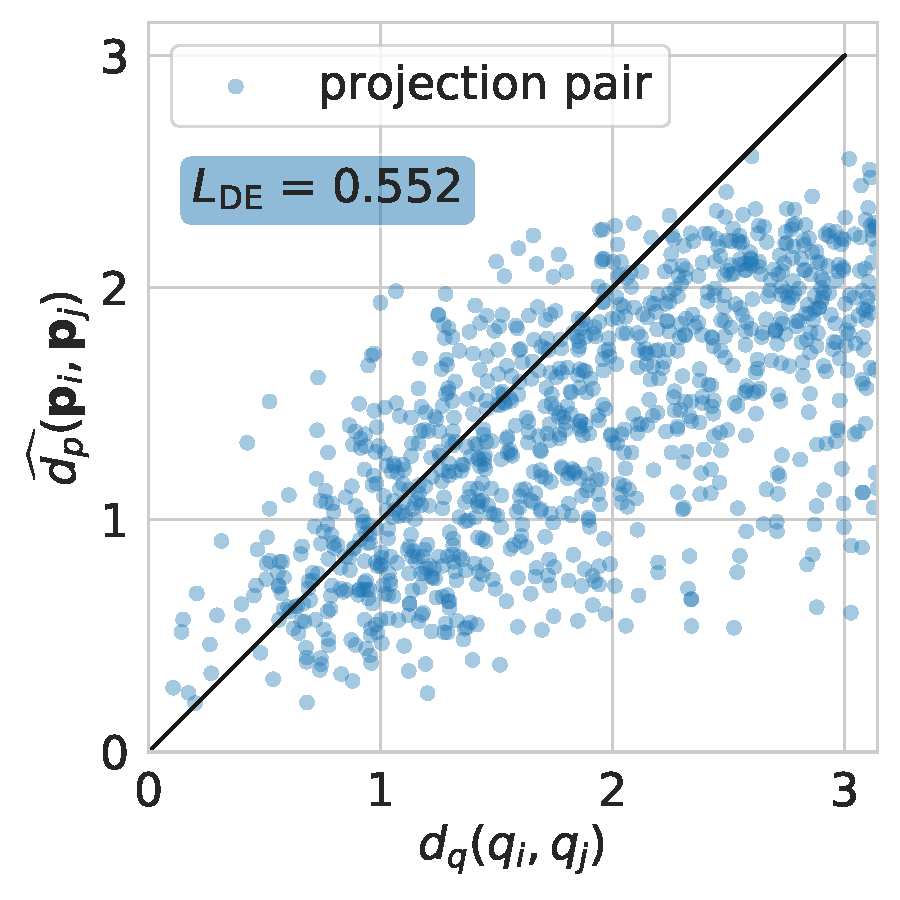
\includegraphics[height=4cm]{figures/dPdQ_5j0n_robustness_to_unseen.pdf}
%         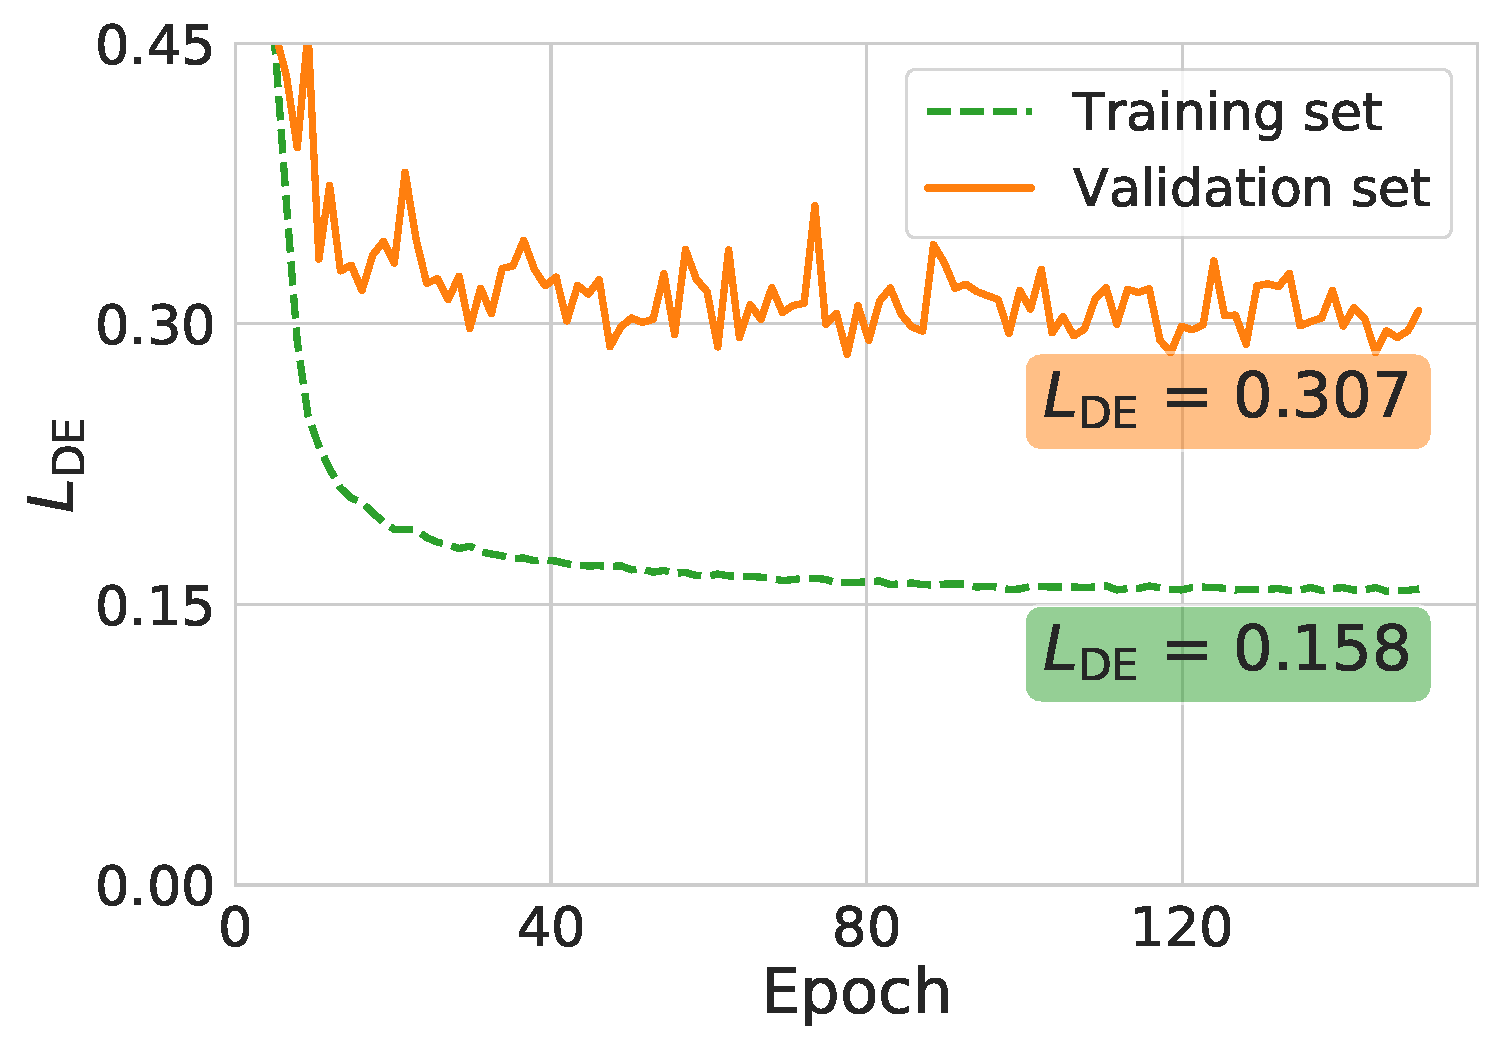
\includegraphics[height=3cm]{figures/de_5j0n_unseen.pdf}
%         \caption{Distance estimation loss on training and validation sets of \texttt{5nvu}, \texttt{5nvs}, \texttt{6mem}, and \texttt{6o1o}.
%             \mdeff{Could we add the validation set of \texttt{5j0n} as a third line? (I'm not sure whether we'll keep it, but it could help us understand what's happening.)}
%             \banjac{I won't have time to rerun it, however, I can report only the test set final loss value. The values in the boxes are the final loss value anyway.}
%         }
%     \end{subfigure}
%     \hfill
%     \begin{subfigure}[t]{0.28\linewidth}
%         \centering
%         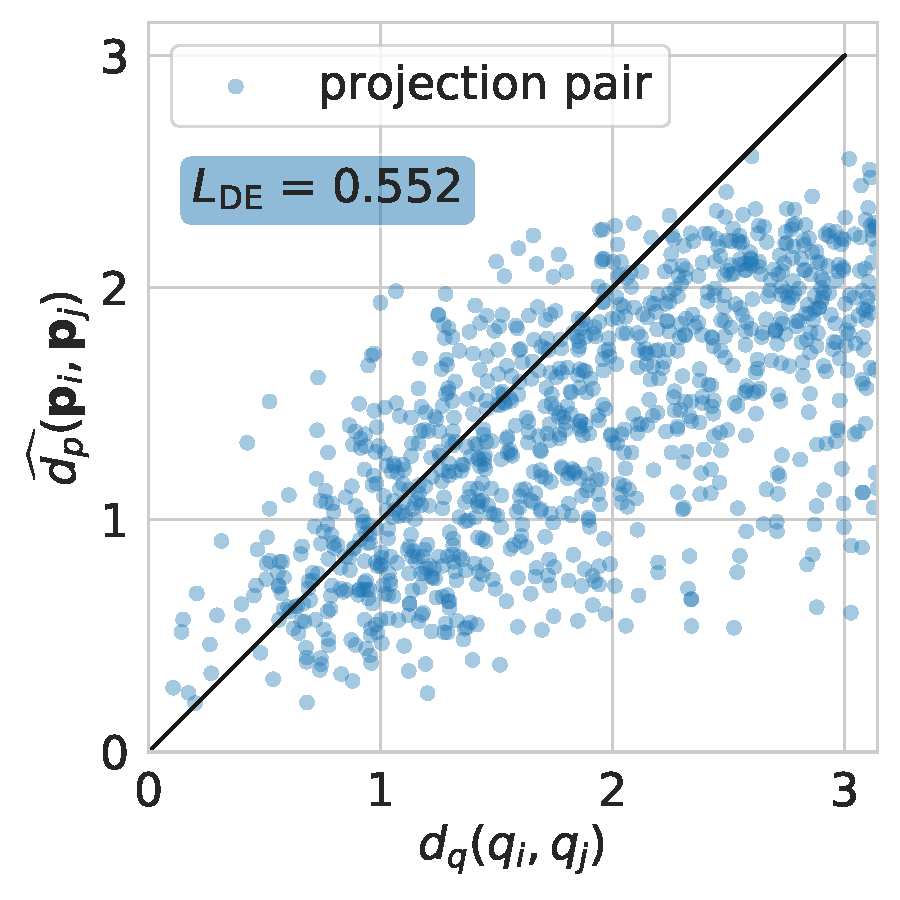
\includegraphics[height=3cm]{figures/dPdQ_5j0n_robustness_to_unseen.pdf}
%         \caption{$\widehat{d_p}$ and $d_q$ relationship on $1,000$ pairs sampled from the test set of \texttt{5j0n}.}
%     \end{subfigure}
%     \hfill
%     \begin{subfigure}[t]{0.35\linewidth}
%         \centering
%         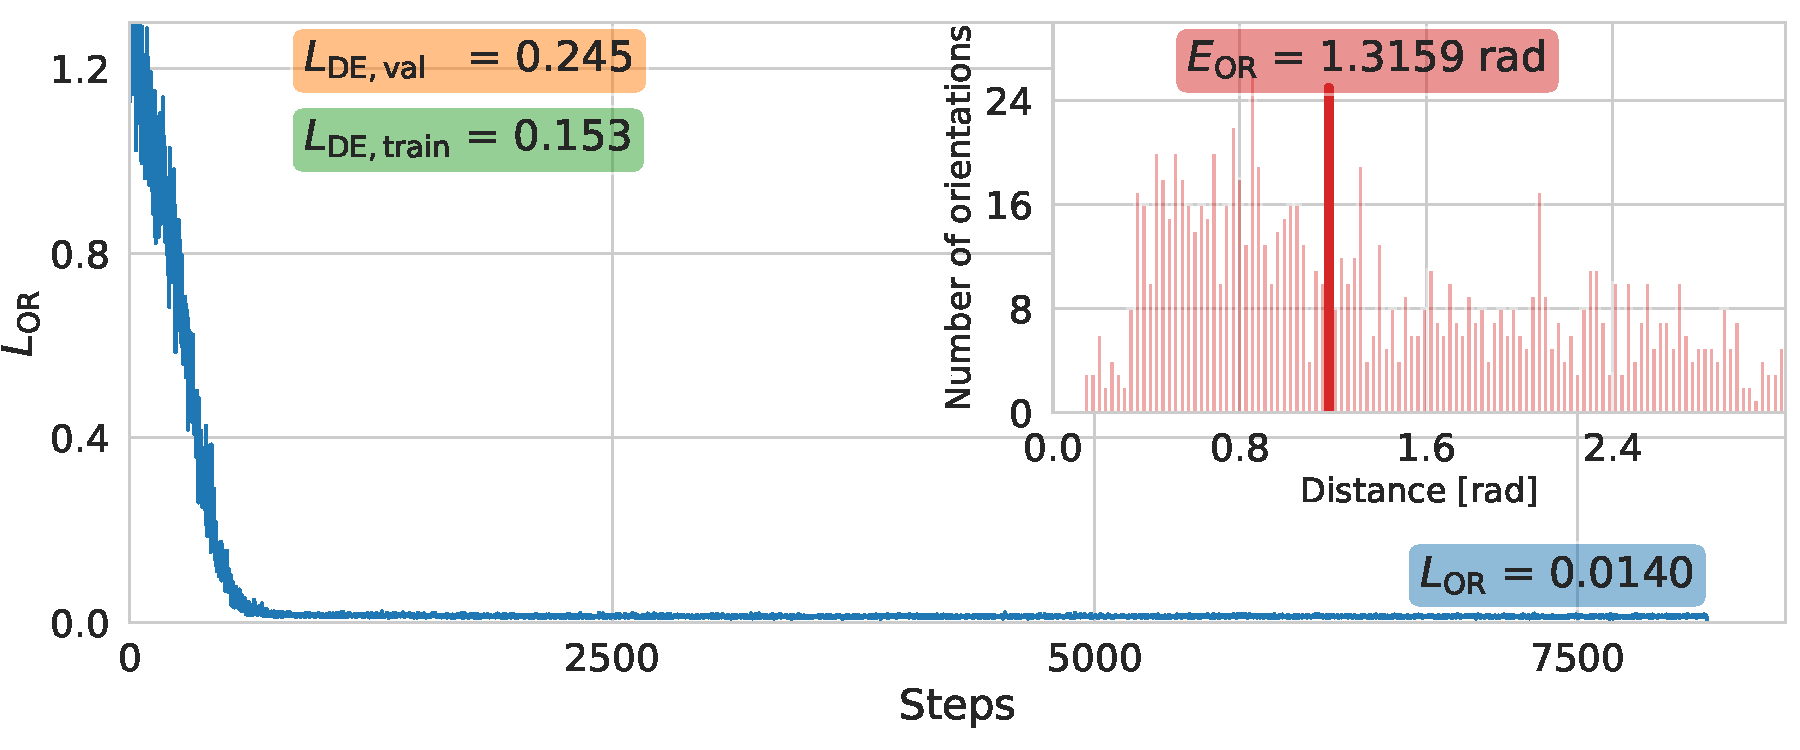
\includegraphics[height=3cm]{figures/5j0n_ar_aa_robustness_to_unseen.pdf}
%         \caption{Recovered $\{ \widehat{q_i} \}$ from noiseless \texttt{5j0n} projections $\{ \p_i \}$ from protein unseen from distance estimation algorithm.}
%     \end{subfigure}
%     \caption{%
%         Robustness to unseen protein \texttt{5j0n} with noiseless projections pipeline results.
%     }\label{fig:robustness-to-unseen-pipeline}
% \end{figure}

\section{SiameseNN: feature distance and embedding dimension}\label{apx:siamese:feature-distance-and-embedding-dimension}

%\mdeff{Story: $d_f = d_q$ better than Euclidean and MLP $d_f$. }

There are multiple options for a distance function $d_f$ between two features $\mathbf{f}_i = \mathcal{G}_w(\p_i) \in \R^{n_f}$.
\figref{geo-eucl-mlp} compares the use of the Euclidean distance $d_f(\f_i, \f_j) = \Vert \f_i - \f_j \Vert_2$ and the cosine distance $d_f(\f_i, \f_j) = 2 \arccos \left( \frac{\langle \f_i, \f_j \rangle}{\lVert \f_i \rVert \lVert \f_j \rVert} \right)$. The cosine distance results in a lower $L_\text{DE}$, which makes $\widehat{d_p}$ a better estimator of $d_q$.
% the projection pairs deviate the least from the identity
This superiority of the cosine distance is likely due to its capacity to model the elliptic geometry of $\SO(3)$, a feat the Euclidean distance does not achieve, the Euclidean space being neither periodic nor curved.
%The $\SO(3)$ is non-linear and it can be explained with the fact that Euclidean distance of two quaternions can be small, despite the rotation being large~\cite{huynh_metrics_2009,DBLP:journals/corr/abs-1805-01026}.
We also tried to parametrize $d_f$ as a multi-layer perceptron (MLP) but were unable to train it.

% The MLP we tested was made of six layers with $1024, 512, 512, 256, 256, 1$ units, all of which use the SeLU activation function.
% The features $\f_i$ and $\f_j$ were stacked as an array of size $2n_f$ before being fed to the MLP\@.
% Note that, while a MLP can approximate any function, there is no guarantee that the learned function will satisfy the axioms of a proper distance function (\ie, the identity of indiscernibles, symmetry, and triangle inequality).

\begin{figure}[ht]
    \centering
    \begin{subfigure}[t]{0.44\linewidth}
        \centering
        % 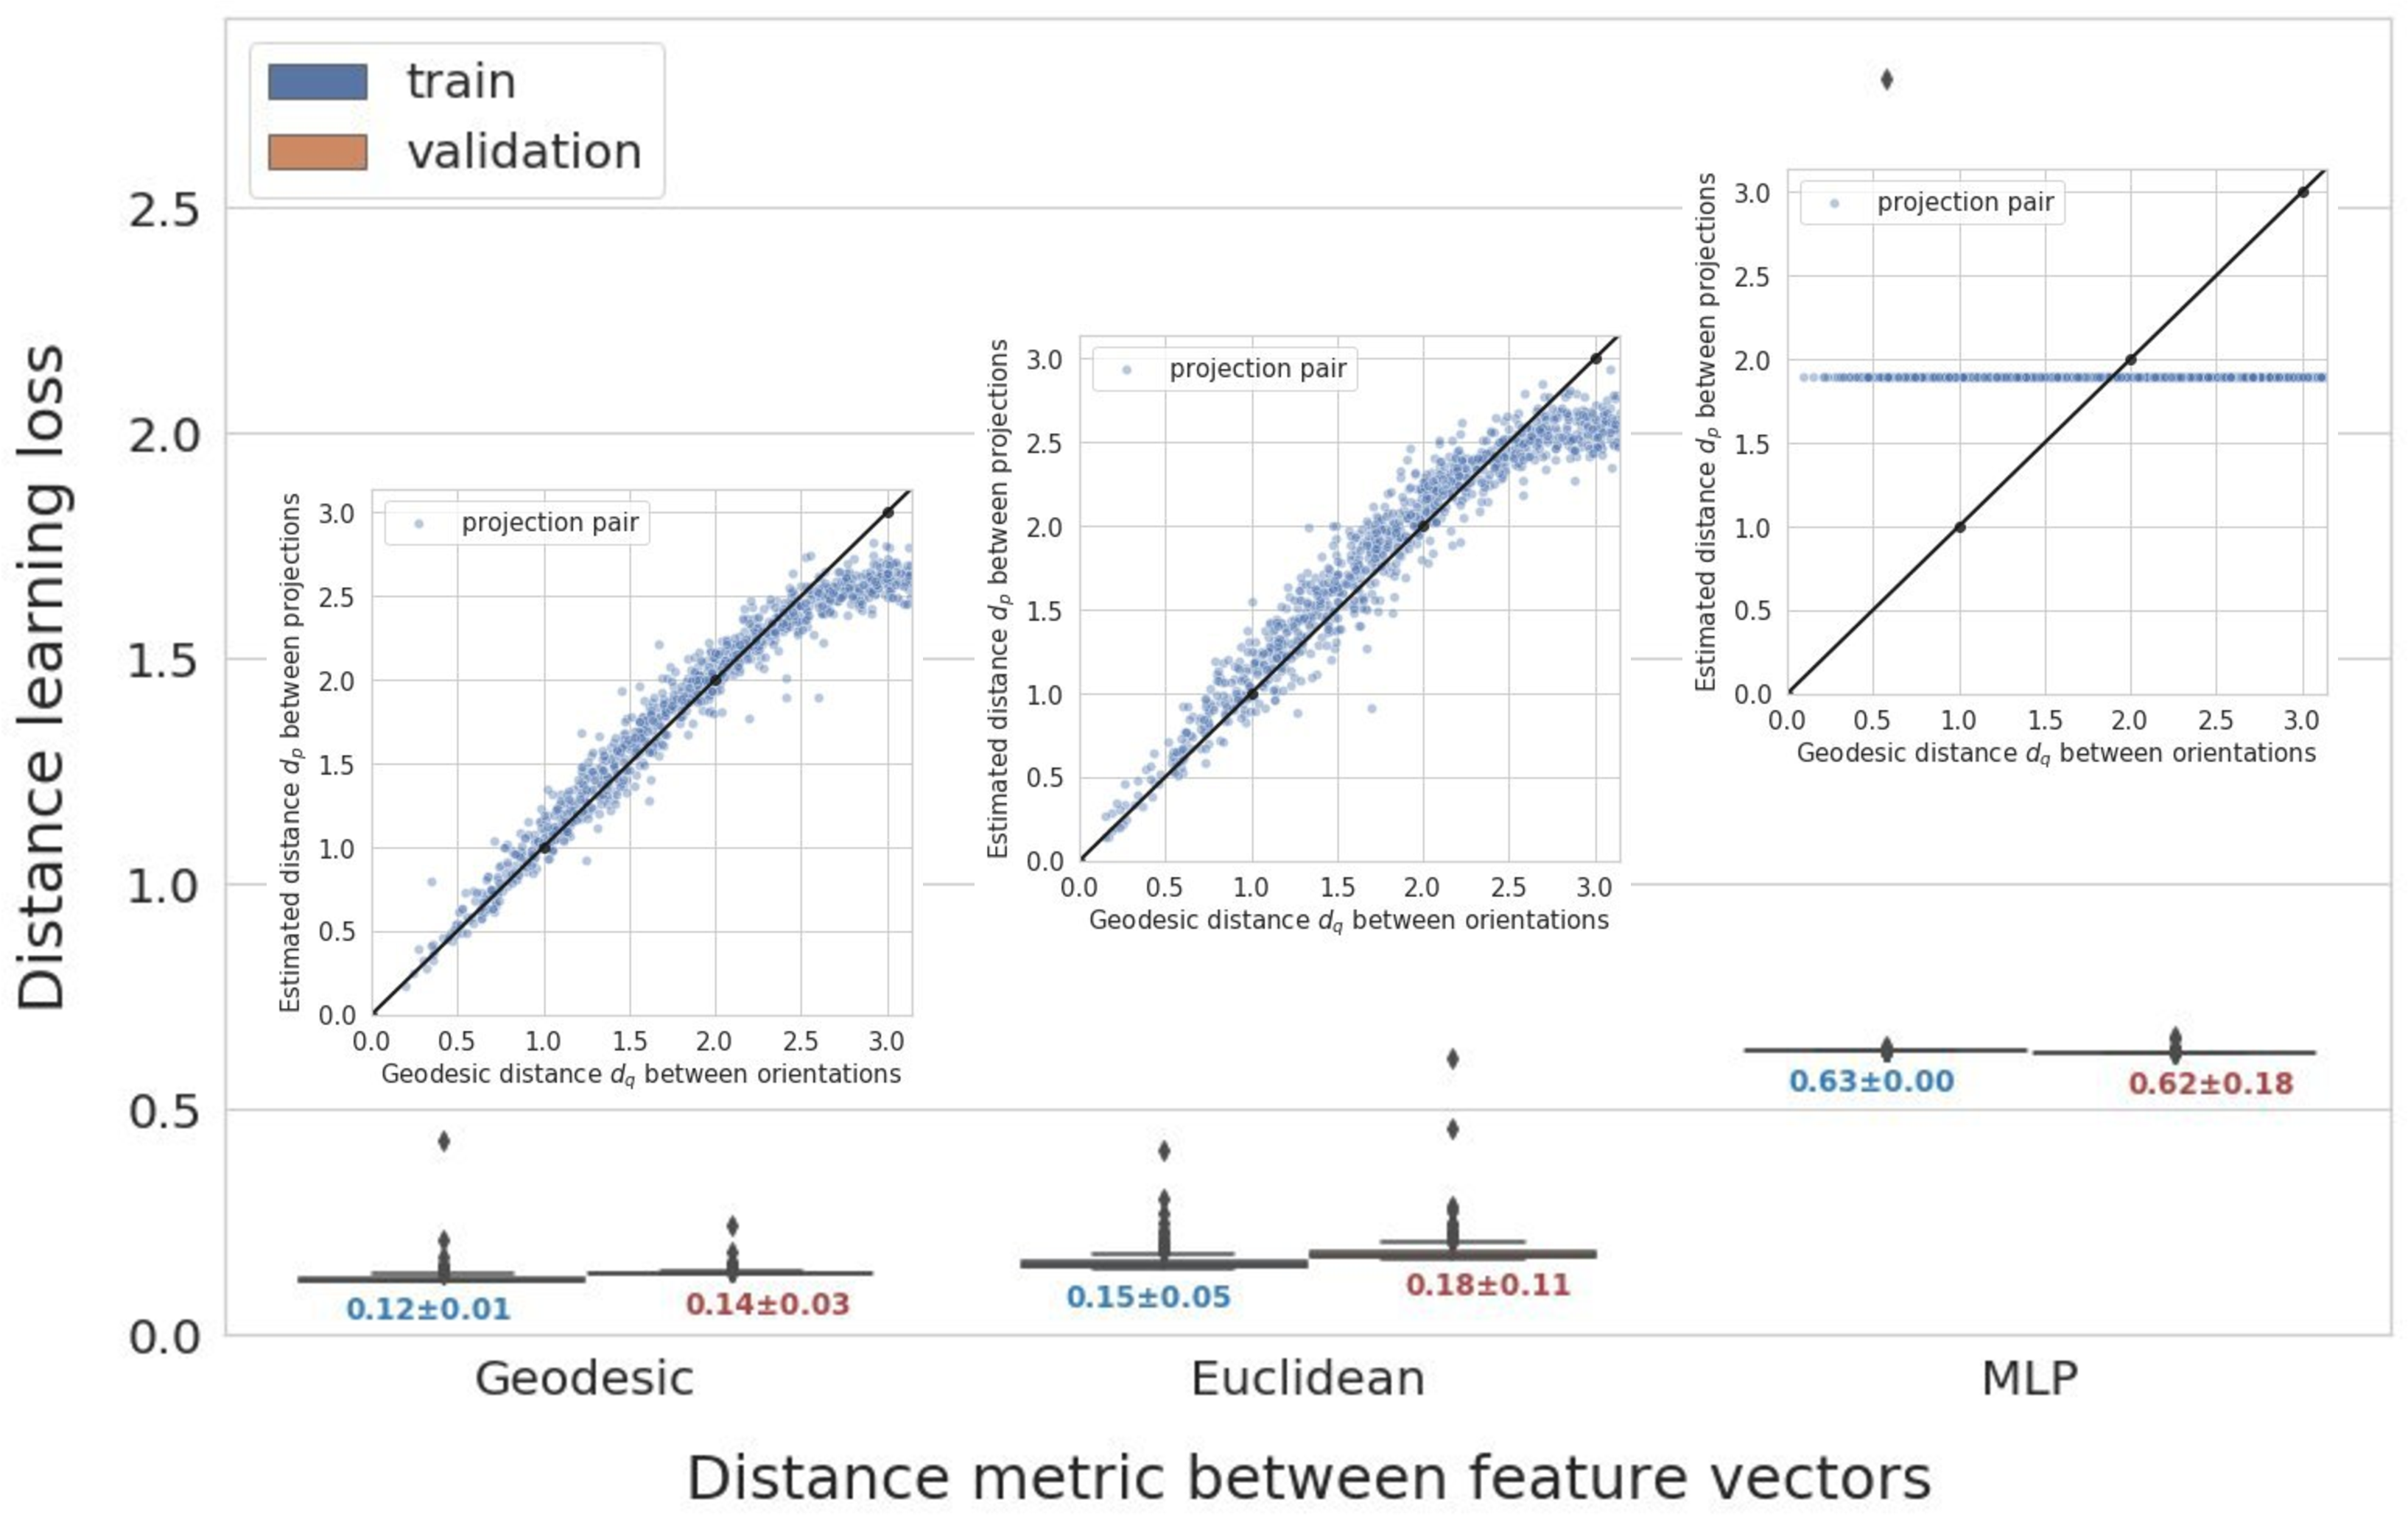
\includegraphics[height=4cm]{figures/geo_eucl_mlp_distance_metric.pdf}
        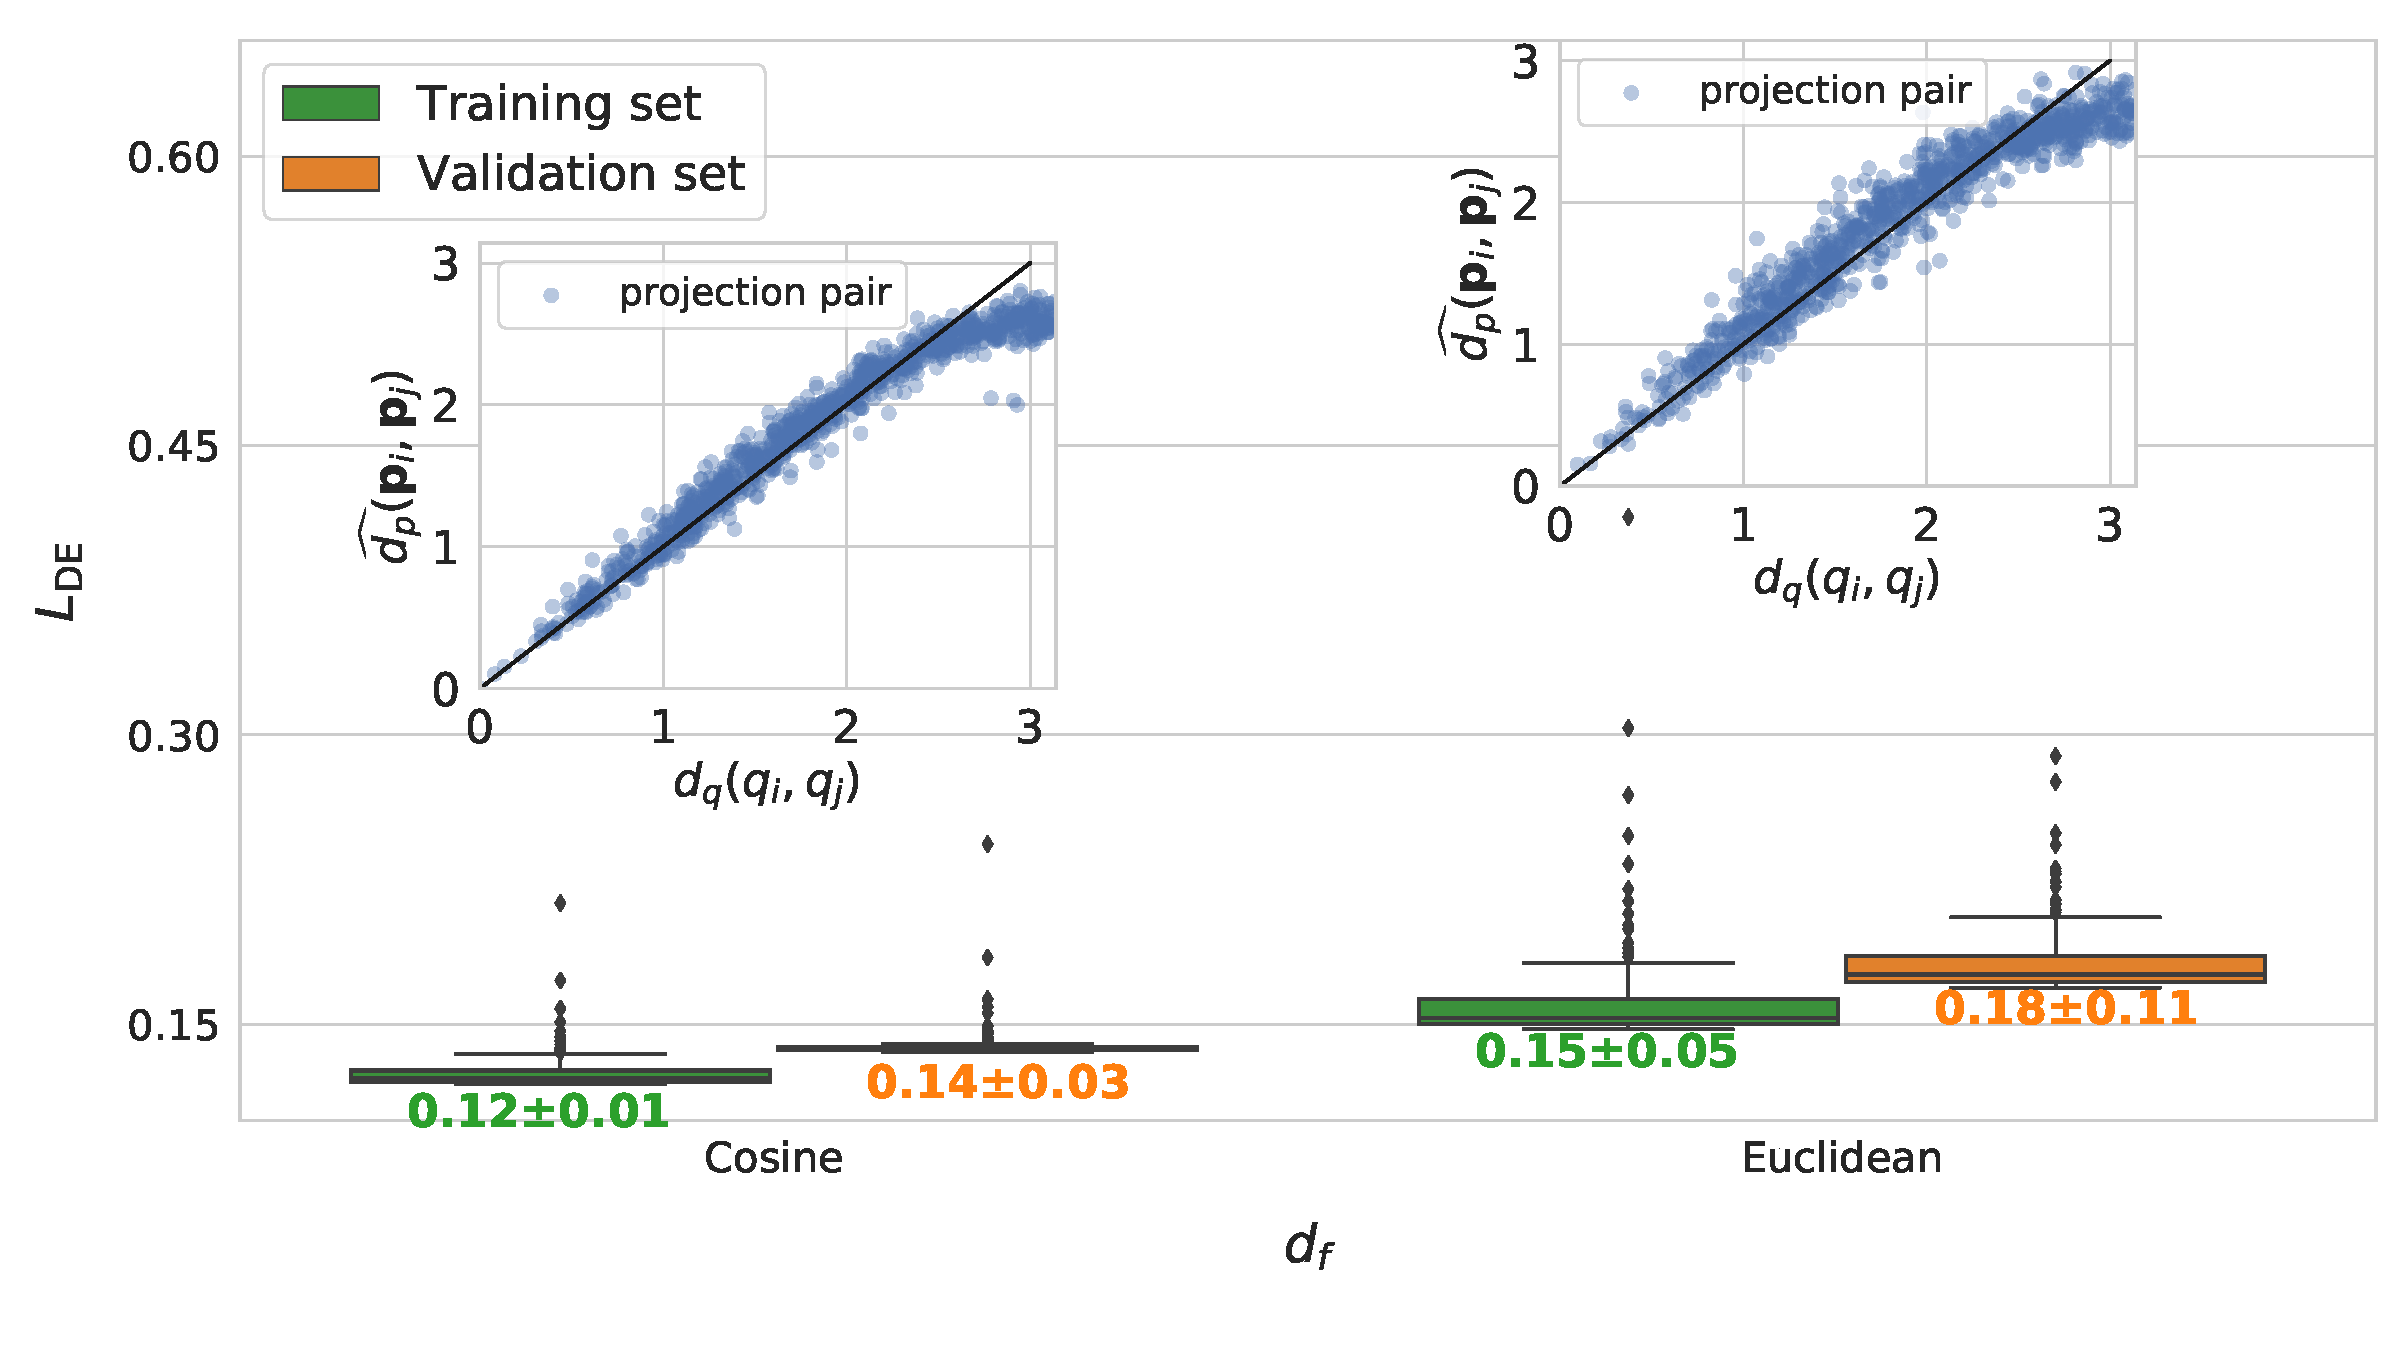
\includegraphics[height=3.5cm]{figures/dPdQ_feat_distances.pdf}
        \caption{%
            Performance w.r.t.\ the feature distance $d_f$.
        }\label{fig:geo-eucl-mlp}
    \end{subfigure}
    \hfill
    \begin{subfigure}[t]{0.51\linewidth}
        \centering
        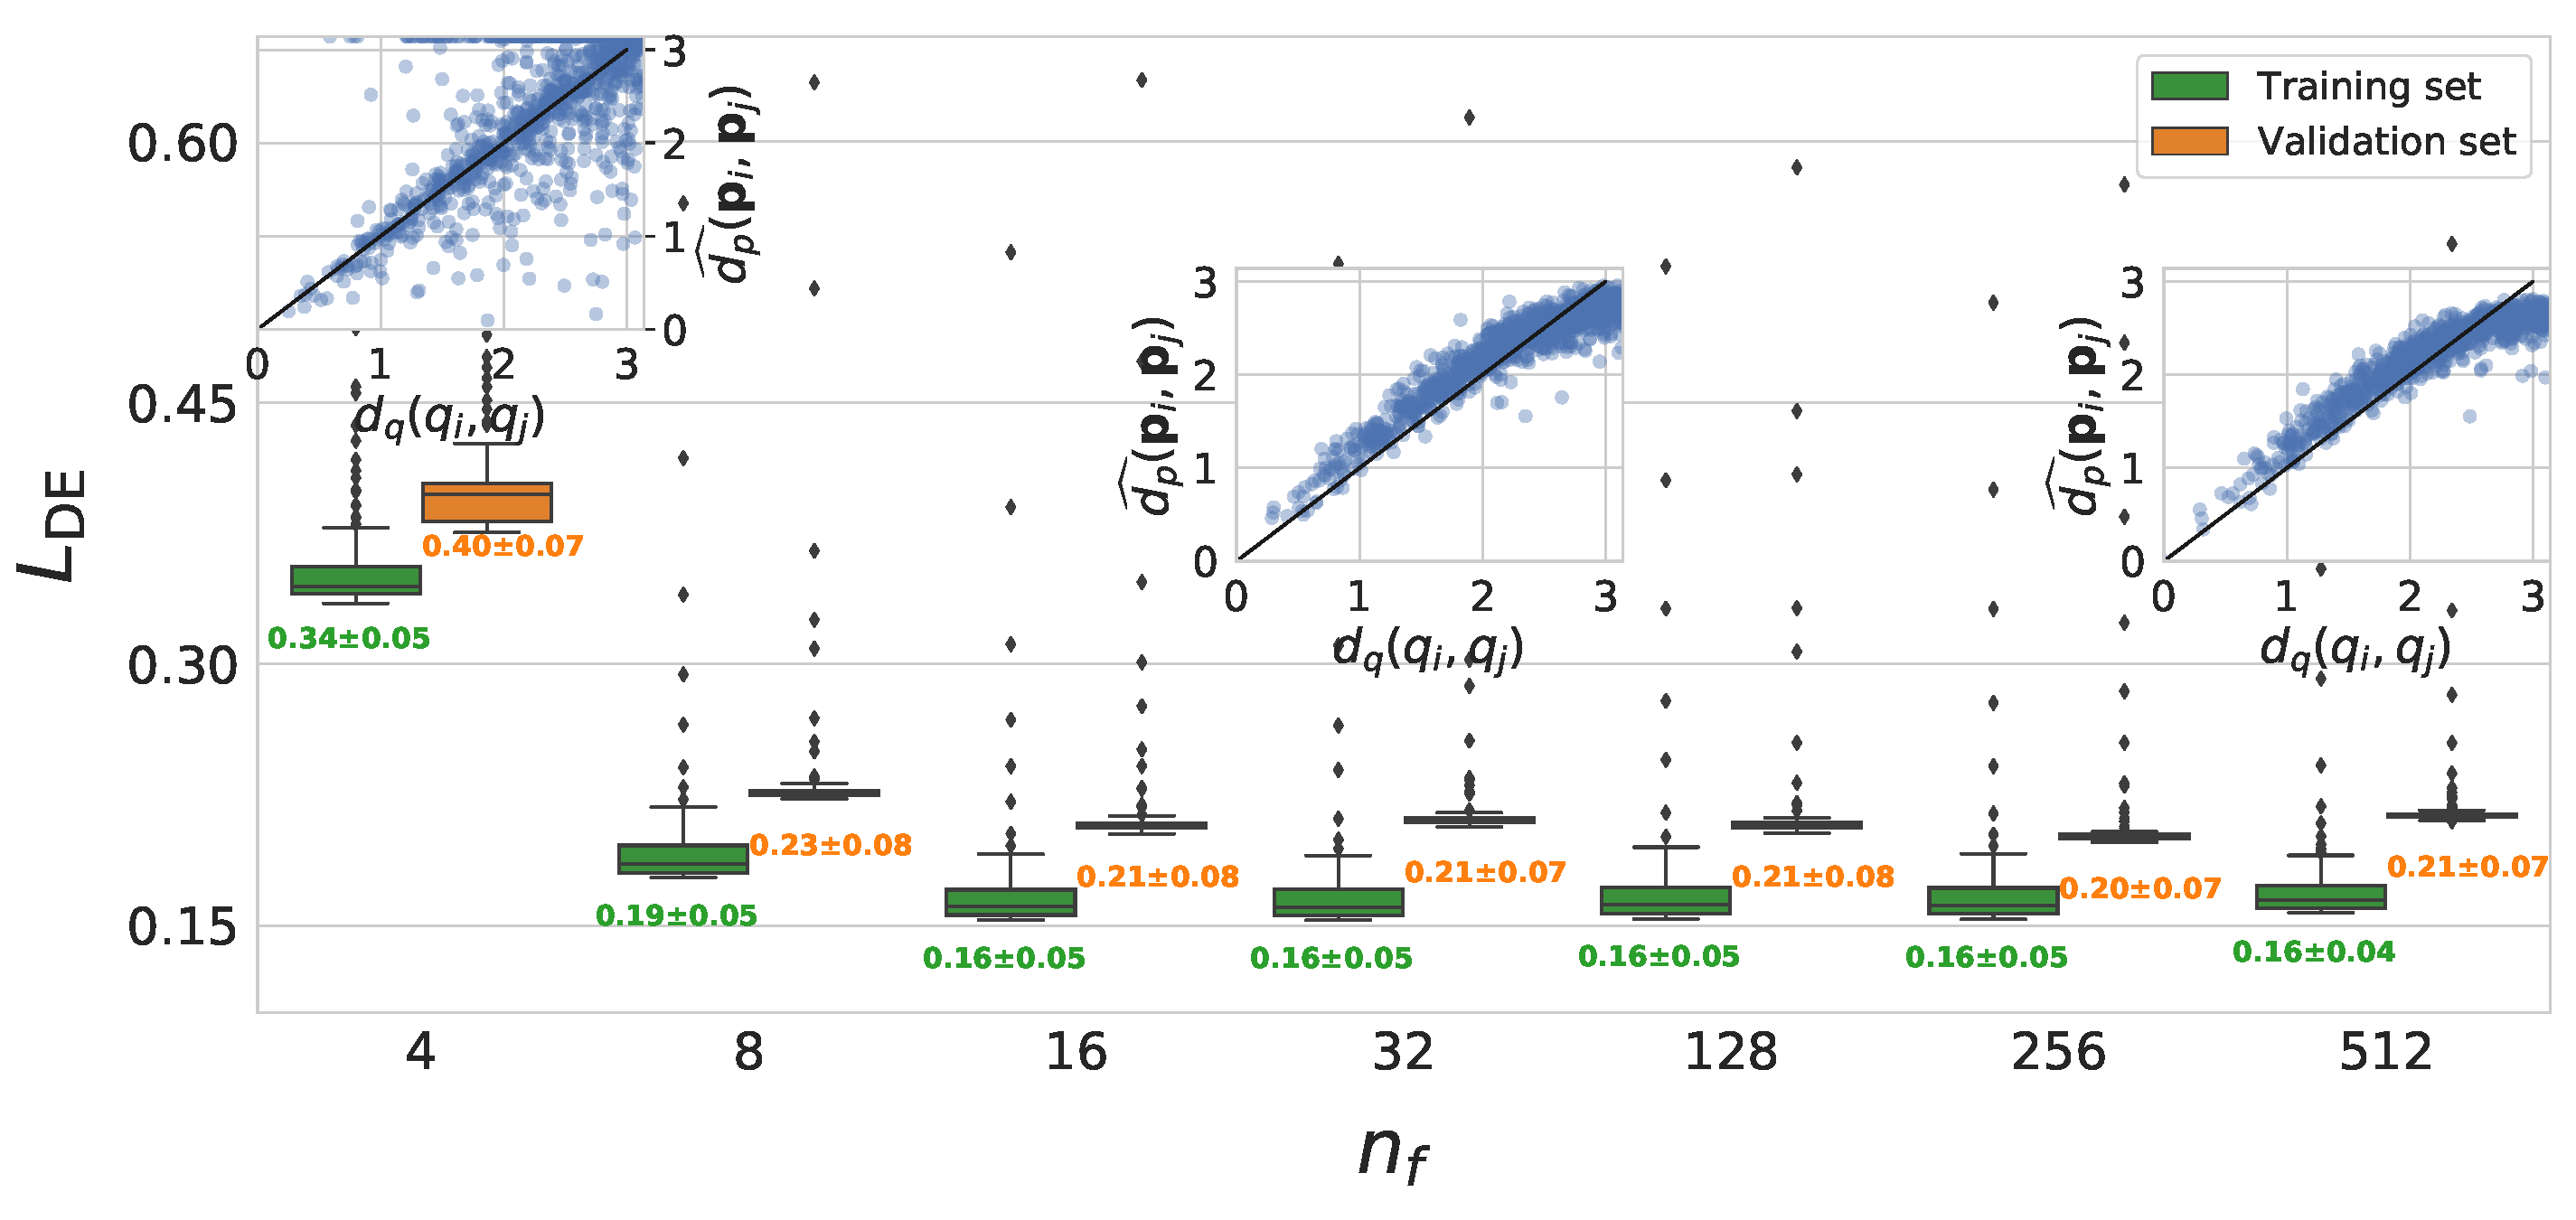
\includegraphics[height=3.5cm]{figures/de_nf.pdf}
        % \begin{subfigure}[t]{0.48\linewidth}
        %     \centering
        %     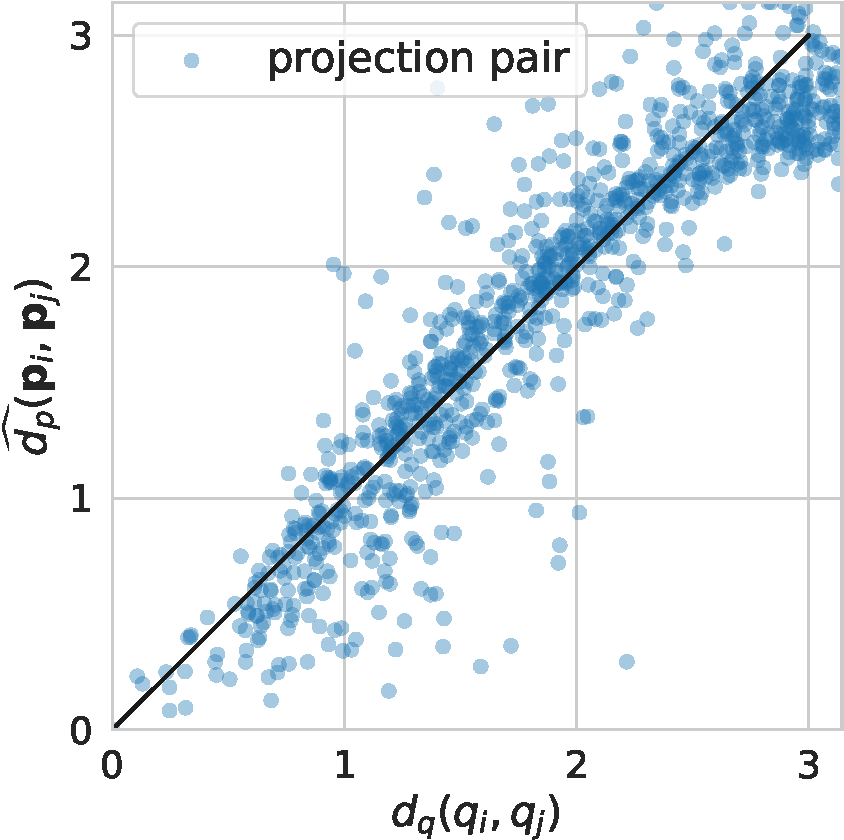
\includegraphics[height=3.5cm]{figures/dPdQ_5j0n_4d.pdf}
        %     \caption*{$n_f=4$} % and half-directions.
        % \end{subfigure}
        % \hfill
        % \begin{subfigure}[t]{0.48\linewidth}
        %     \centering
        %     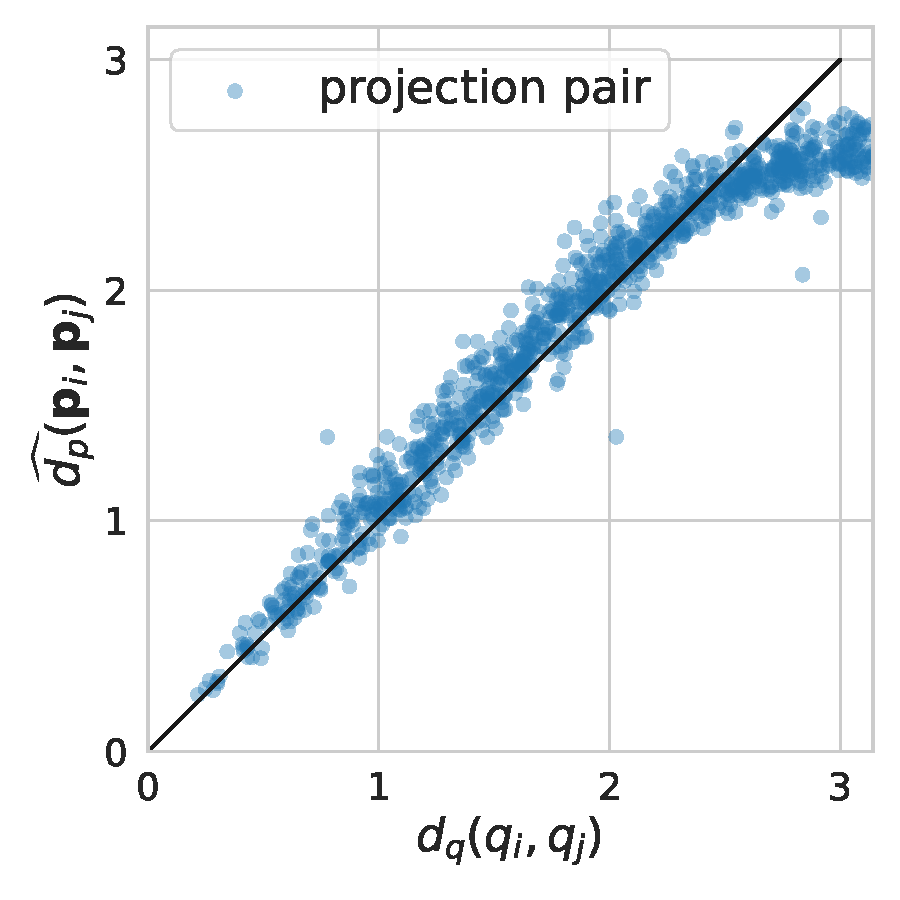
\includegraphics[height=3.5cm]{figures/dPdQ_5j0n_256.pdf}
        %     \caption*{$n_f=256$} % and half-directions.
        % \end{subfigure}
        % % \hfill
        % % \begin{subfigure}[t]{0.31\linewidth}
        % %     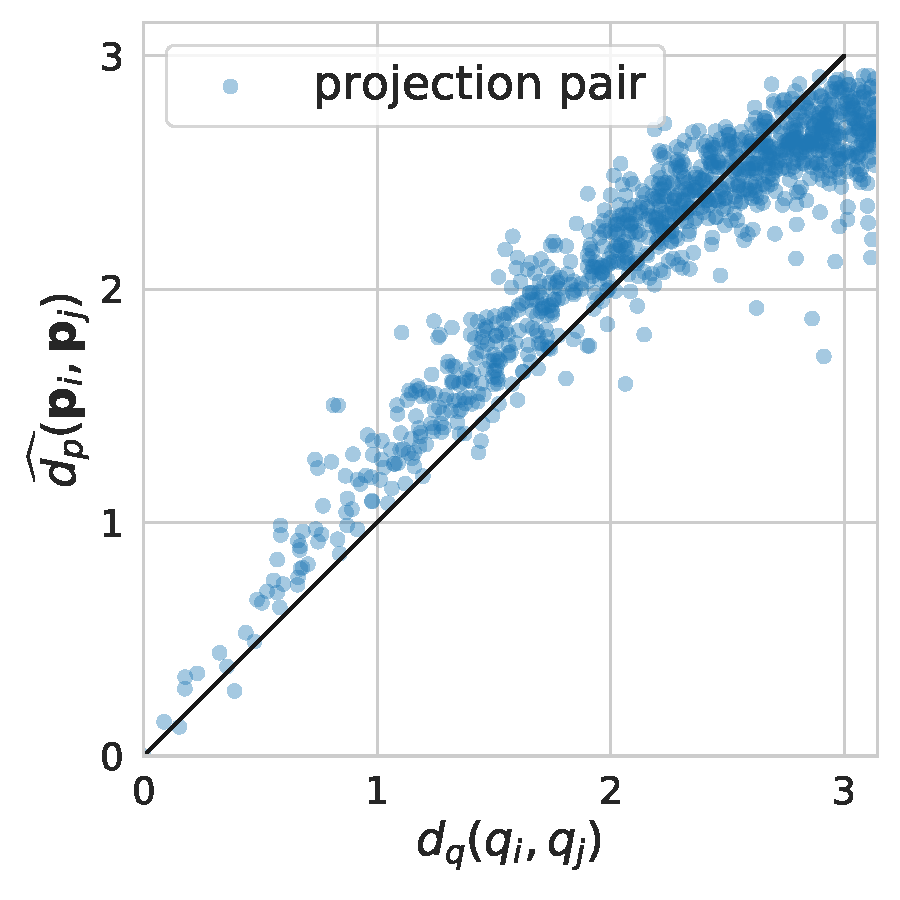
\includegraphics[width=\linewidth]{figures/dPdQ_5j0n_full.pdf}
        % %     \caption{$n_f=256$ and all-directions.}
        % % \end{subfigure}
        \caption{%
            Performance w.r.t.\ the embedding dimensionality $n_f$.
            %Different direction constrains in \figref{orientation-constraints}.
            %\todo{Very interesting: 4 is not enough but 8 already is.}
        }\label{fig:4d-vs-256d-de}
    \end{subfigure}
        \caption{%
            Performance of our distance estimator $\widehat{d_p}$ w.r.t.\ two design choices.
            The box plots show the distance learning loss $L_\text{DE}$ \eqnref{distance-learning}.
            The inserted plots show the relationship between $d_p(\p_i, \p_j) = d_f(\mathcal{G}_w(\p_i), \mathcal{G}_w(\p_j))$ and $d_q(q_i, q_j)$ on $1,000$ pairs sampled from \texttt{5j0n}.
        }
\end{figure}

\figref{4d-vs-256d-de} shows the performance of our distance estimator $\widehat{d_p}$ depending on the size $n_f$ of the feature space.
It clearly indicates that a space of $n_f=4$ dimensions is insufficient to represent the variability of projections.
% $n_f=4$ dimensional space is too constrained
That is a motivation to embed the projections in a space of higher dimensions that can represent more variations than the orientation, and can abstract that variation by solely considering the distances between the embedded projections $\f_i = \G_w(\p_i)$.
While our choice of $n_f=512$ might be overkill ($n_f=16$ seems sufficient), it is not penalizing.
%Great motivation for our indirect method and $n_f>4$, even when trained and tested on the same protein.
%Difference in the architecture of networks with $n_f=4$ or $n_f=256$ is in \apxref{siamese-architecture}.

\section{Convolutional neural network architecture}\label{apx:siamese-architecture}

\begin{figure}[ht!]
    \centering
    \begin{subfigure}[t]{1.0\linewidth}
        % 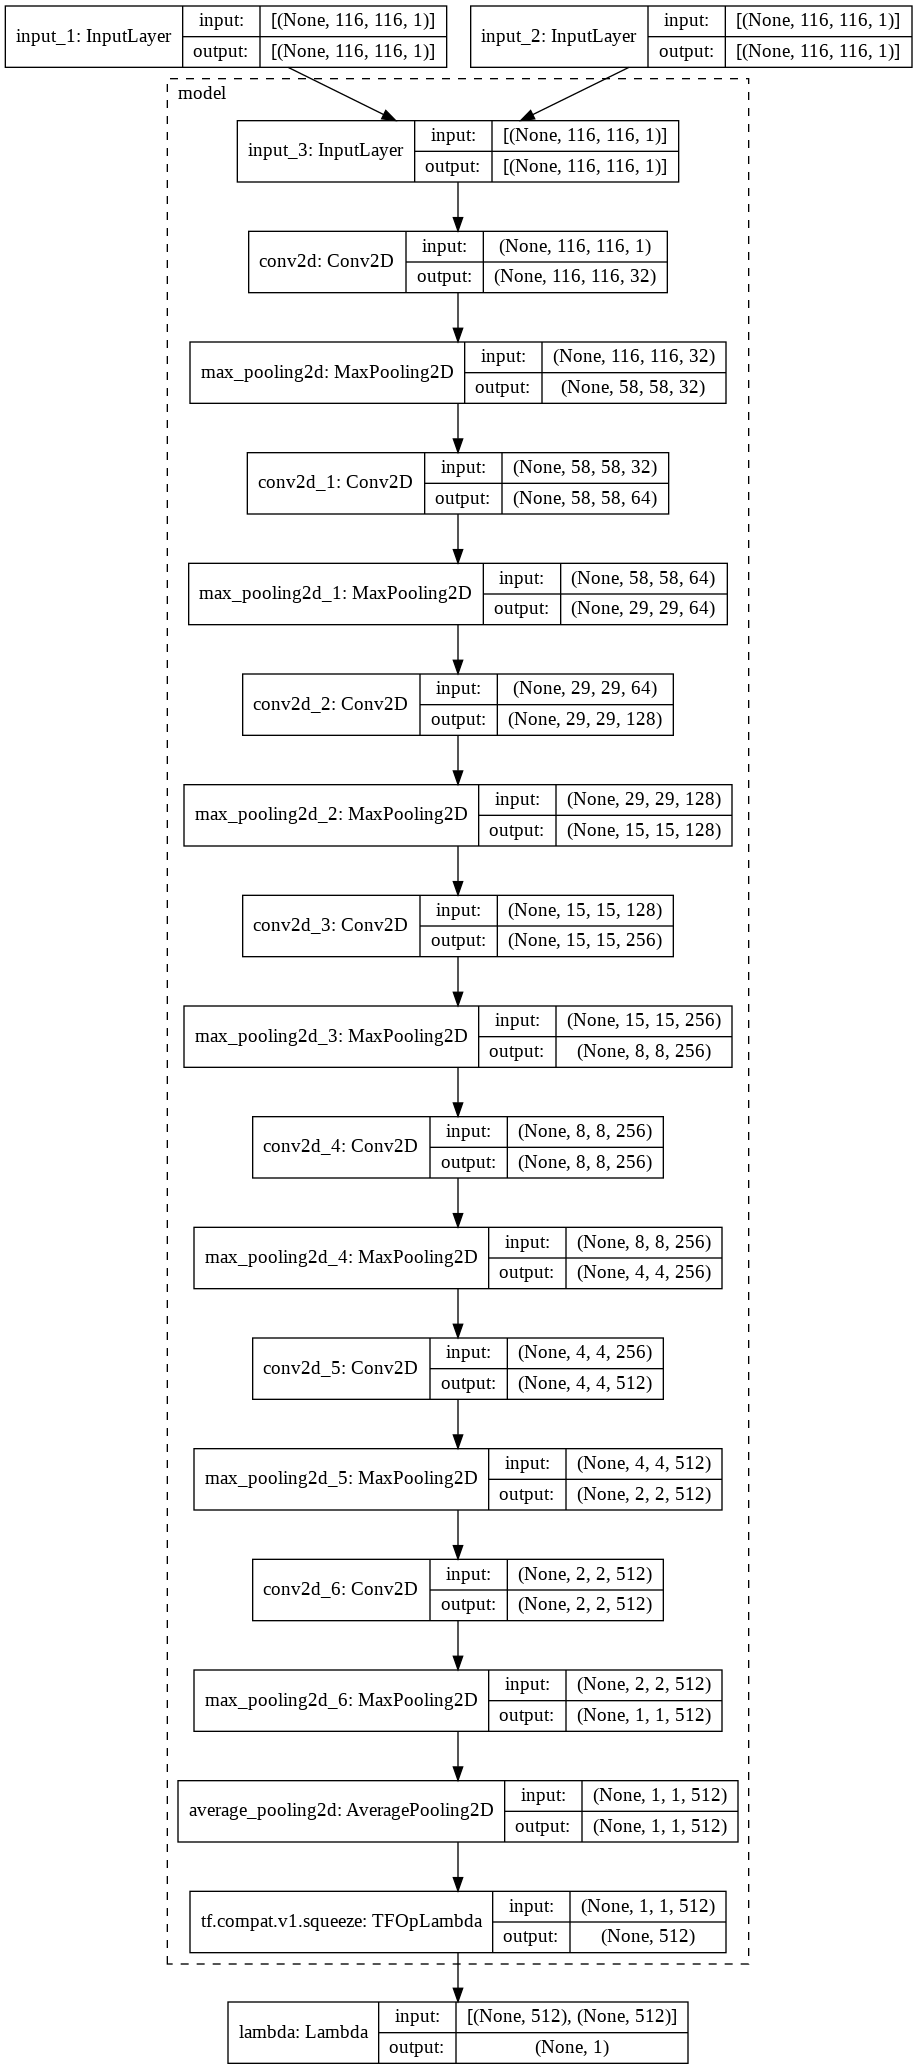
\includegraphics[width=\linewidth]{figures/model_plot_256d.png}
        %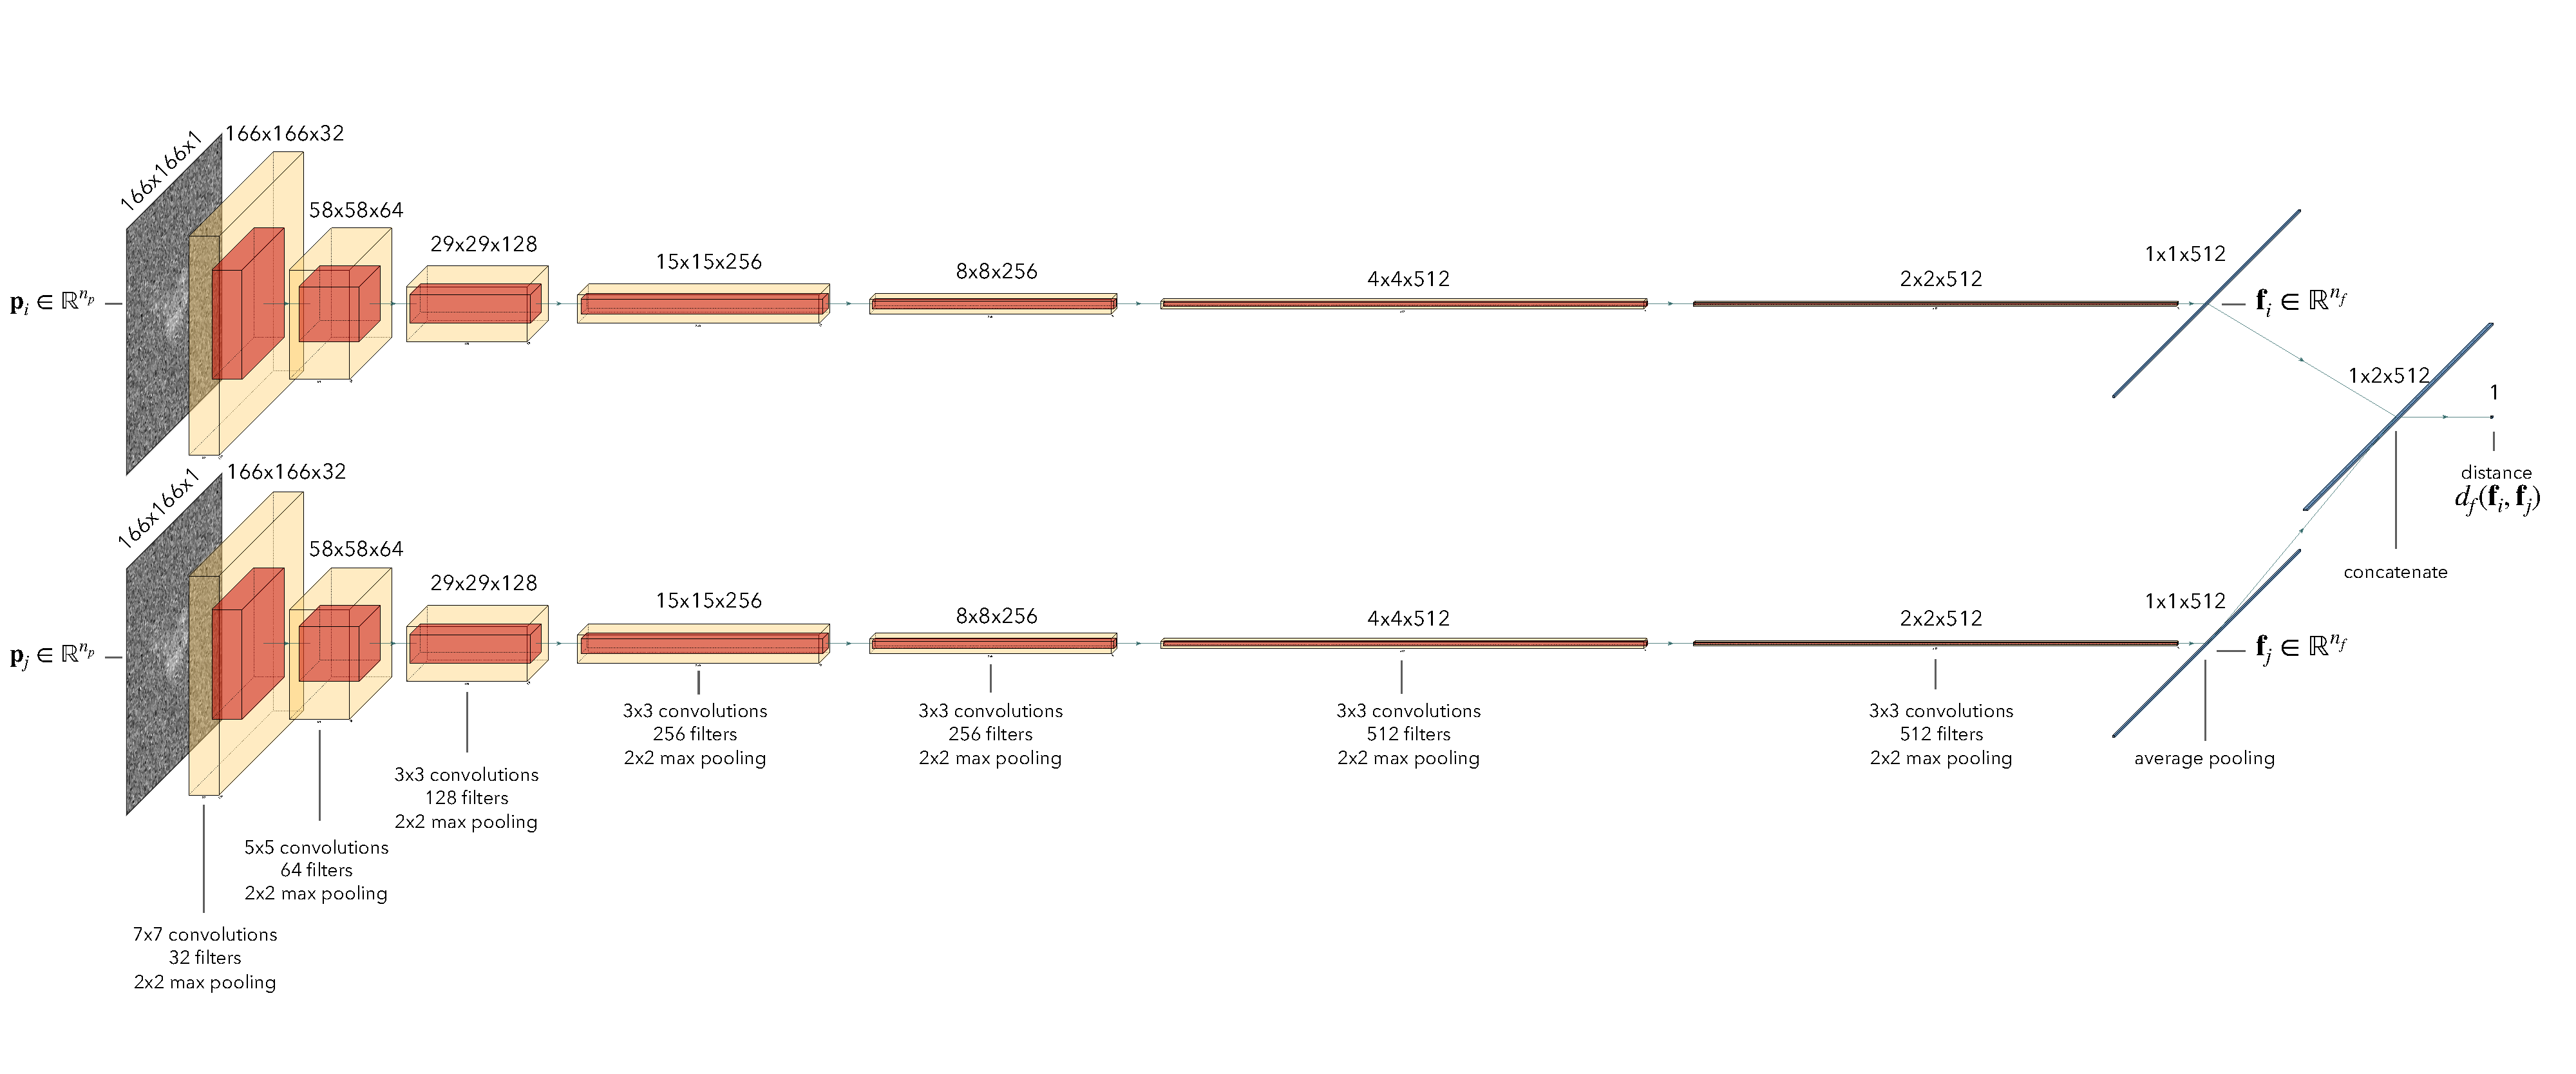
\includegraphics[width=\linewidth]{figures/architecture.pdf}
        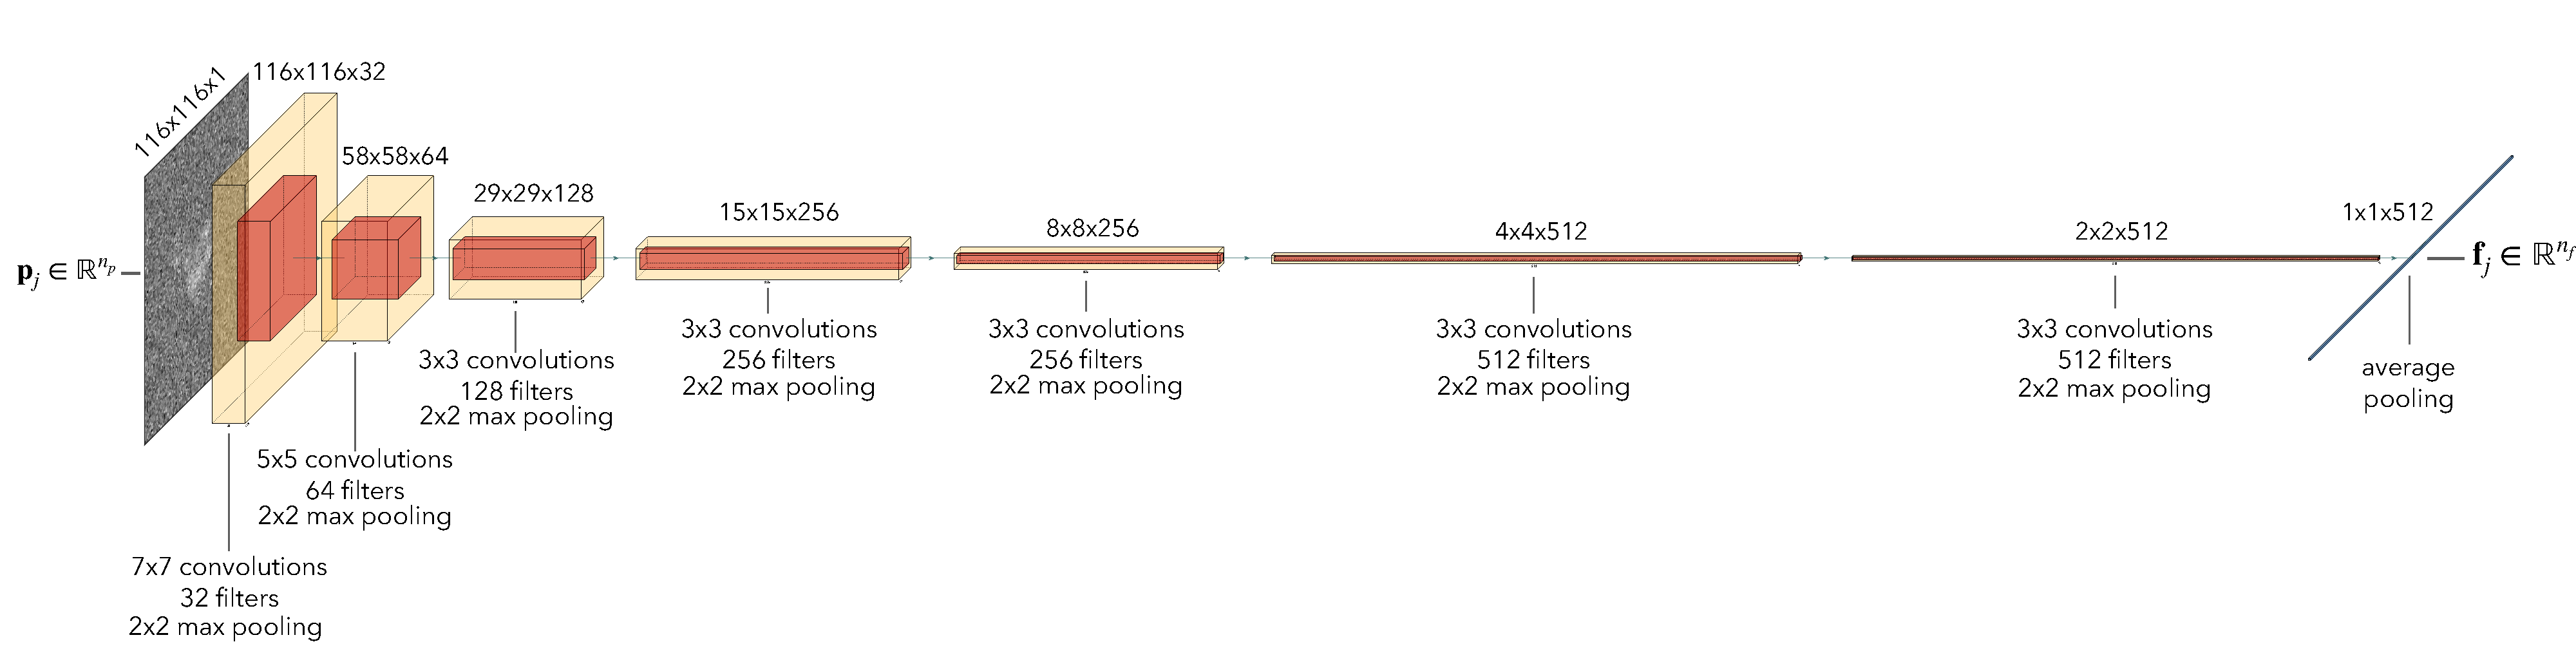
\includegraphics[width=\linewidth]{figures/architecture2.pdf}
    \end{subfigure}
    \caption{%
        Architecture of $\mathcal{G}_w$, the convolutional neural network that extracts feature vectors $\f_j = \mathcal{G}_w(\p_j) \in \R^{n_f}$ from projections $\p_j \in \R^{n_p}$.
        While $n_f=512$ and $n_p=116 \times 116$ in our experiments, $\mathcal{G}_w$ can accommodate any image size thanks to the global average pooling layer.
    }\label{fig:de-architecture}
\end{figure}
